\documentclass[10pt,a4paper,oneside,openany]{book}
\usepackage[margin=22mm,headheight=15pt]{geometry}
\usepackage{fontspec}
\setmainfont{DejaVu Serif}
\setsansfont{DejaVu Sans}
\setmonofont{DejaVu Sans Mono}[Scale=0.88]
\usepackage{microtype}
\usepackage{xcolor,graphicx,longtable,booktabs,array,fvextra,enumitem,fancyhdr,tikz}
\usetikzlibrary{positioning,arrows.meta}
\usepackage[unicode,colorlinks=true,linkcolor=teal,urlcolor=teal,bookmarksnumbered=true]{hyperref}
\usepackage{bookmark}
\pdfstringdefDisableCommands{\def\allowbreak{}}
\definecolor{ink}{HTML}{16313A}
\definecolor{teal}{HTML}{147B74}
\setlength{\parindent}{0pt}
\setlength{\parskip}{5pt}
\setlength{\emergencystretch}{3em}
\raggedbottom
\setlist{nosep,leftmargin=*}
\renewcommand{\arraystretch}{1.18}
\setlength{\tabcolsep}{4pt}
\pagestyle{fancy}
\fancyhf{}
\fancyhead[L]{\small\sffamily Genrmination\_Fight}
\fancyhead[R]{\small\sffamily Design and engineering record}
\fancyfoot[L]{\scriptsize Snapshot: 14 September 2026}
\fancyfoot[R]{\thepage}
\hypersetup{pdftitle={Genrmination_Fight: Design, Engineering and Complete Source},pdfauthor={Prepared by Codex for the project owner},pdfsubject={Evidence-based game design document and technical annex}}
\setcounter{tocdepth}{1}
\begin{document}
\frontmatter
\begin{titlepage}
\color{ink}\sffamily
\vspace*{16mm}
{\large ROBLOX EXPERIENCE DOCUMENTATION\par}
\vspace{12mm}
{\fontsize{34}{39}\selectfont\bfseries Genrmination\_Fight\par}
\vspace{7mm}
{\LARGE Design, engineering, and complete source\par}
\vspace{15mm}
\rule{\textwidth}{1pt}
\vspace{7mm}
{\large From the supplied design template, development conversations, latest export, and live Studio source.\par}
\vspace{10mm}
{\large 21 active sources\quad 8 archived sources\quad 13 photographs\par}
{\large 1 disabled generator\quad 12 historical workspace artifacts\par}
\vfill
{\large Snapshot edition: 14 September 2026\par}
{\normalsize Place 137098589879404 / version 77 baseline + Revision 5 repairs\par}
\vspace{5mm}
{\small Includes open defects, historical test limits, future implementation recipes, and full line-numbered code. Live repairs and embedded engineering comments included. Revision 5 reverses the Revision 4 geometry migration, rebuilds carrier navigation on the live map, and replaces the passive opposition with a hostile ambush. Not published.\par}
\end{titlepage}
\tableofcontents
\mainmatter
\part{Game design and engineering record}
\chapter{The game as it plays: environment, cast, equipment and tactics}

Every photograph in this chapter was taken from the live place on 14 September
2026, by driving the Studio camera to the stated position and capturing the
viewport.\ Nothing is a mock-up or a render of a plan.\

\section{Photographic survey}

\begin{figure}[htbp]\centering
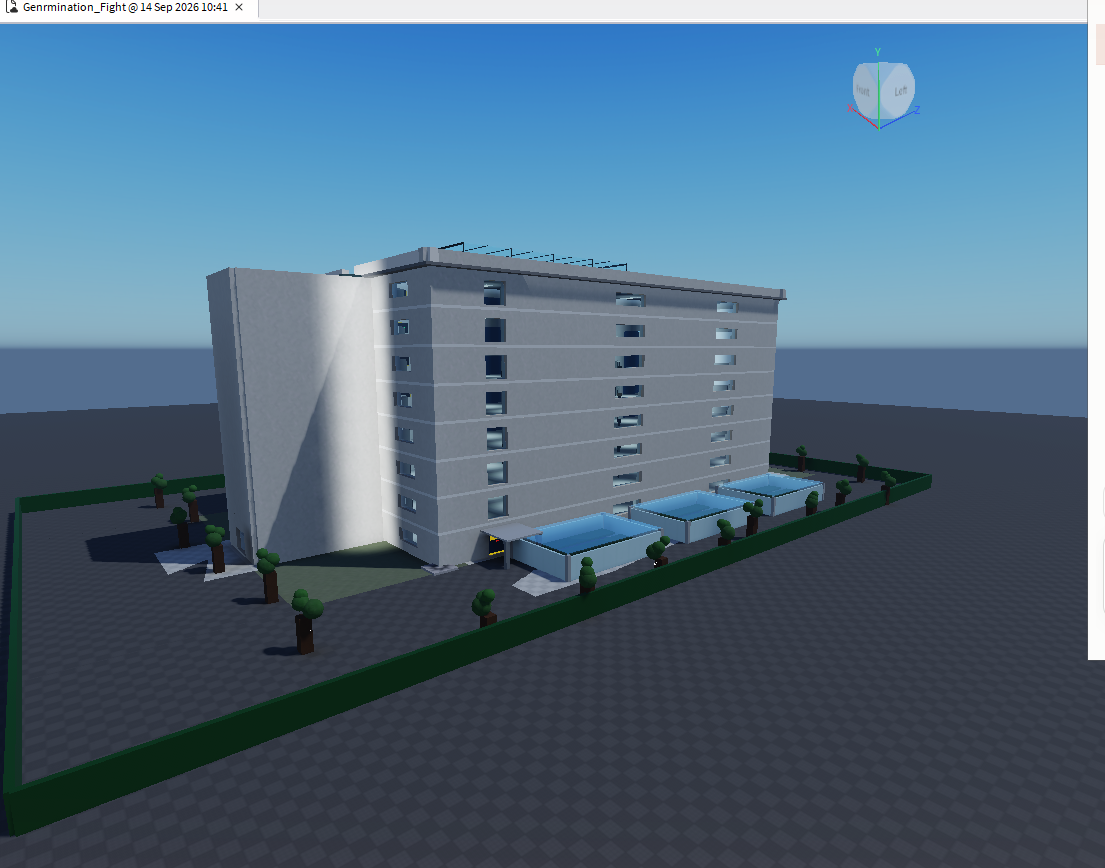
\includegraphics[width=0.92\textwidth]{figures/shots/fig01-exterior.png}
\caption{The laboratory from the south-west approach. Eight storeys above grade
over a basement, inside a fenced compound. The three blue-glazed structures on
the apron are the ground-level glasshouses; the darker strip at the near corner
is the entrance canopy.}
\end{figure}

\begin{figure}[htbp]\centering
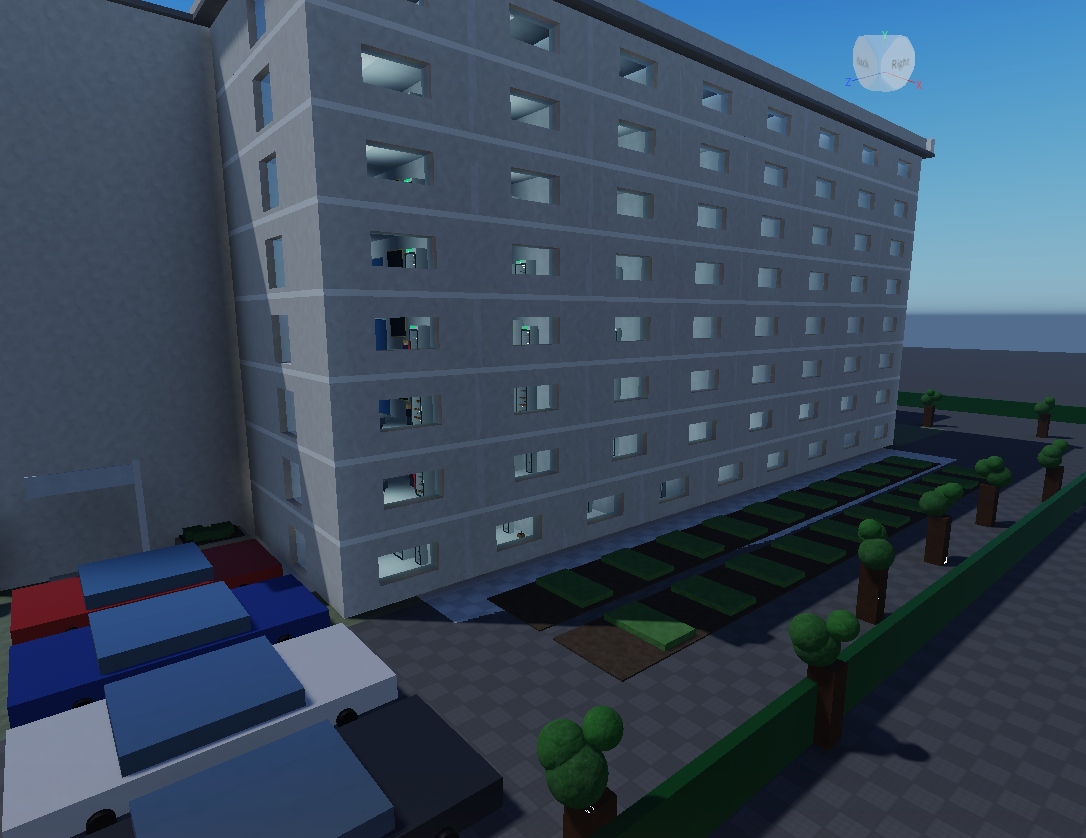
\includegraphics[width=0.92\textwidth]{figures/shots/fig02-siteworks.png}
\caption{Site works from the north-east: perimeter fence and gate, parking bays
with four vehicles, planters, flagpole, trial plots and twenty-eight trees
planted in bands that avoid the building footprint and the aprons.}
\end{figure}

\begin{figure}[htbp]\centering
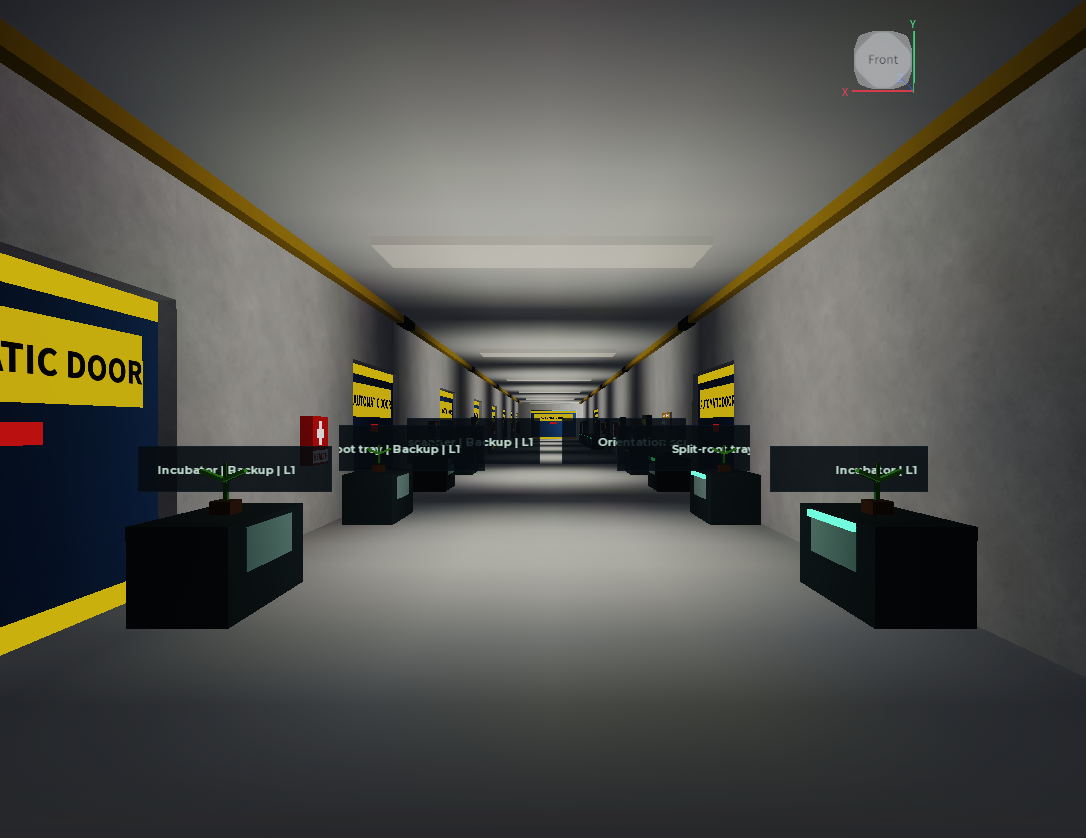
\includegraphics[width=0.92\textwidth]{figures/shots/fig03-corridor.png}
\caption{A typical floor corridor, looking north along Level 1. Research
stations stand against both walls with their own labels and status lights;
automatic doors are marked in yellow and blue; emergency kits are the red
cabinets. The corridor is the spine of every floor and the only continuous
route between the two stair towers.}
\end{figure}

\begin{figure}[htbp]\centering
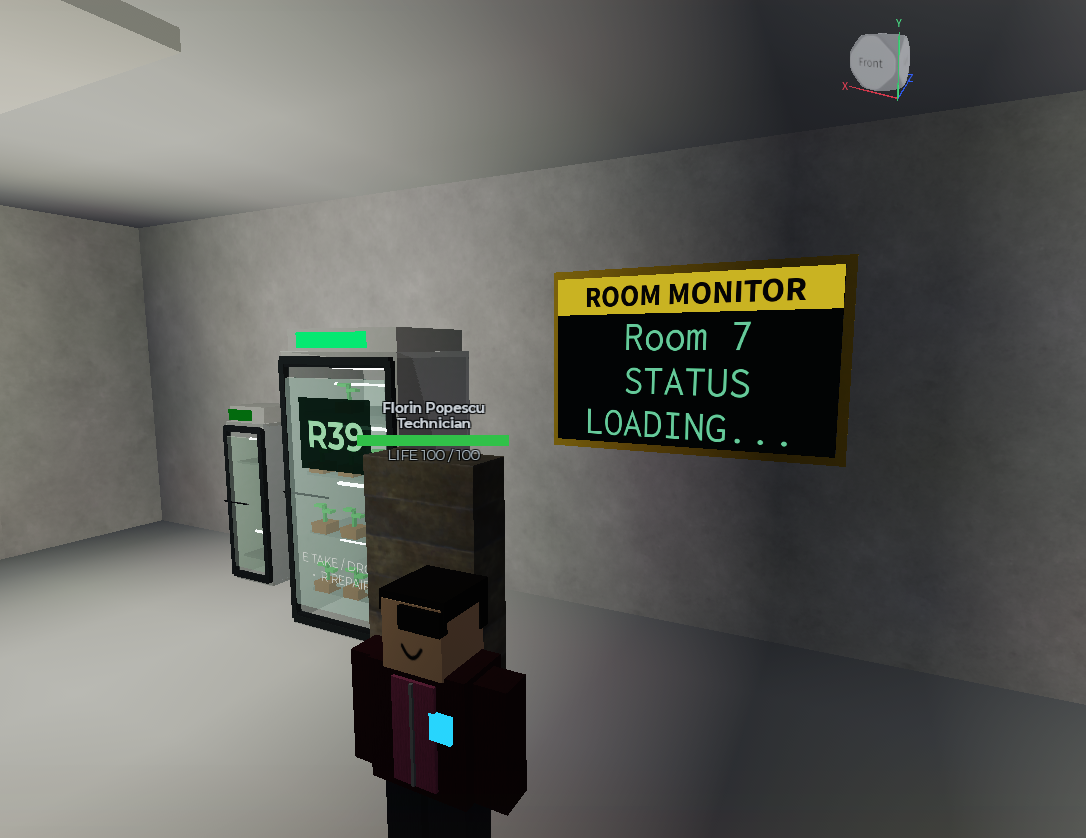
\includegraphics[width=0.92\textwidth]{figures/shots/fig04-growthchambers.png}
\caption{Inside a laboratory room. The germination chambers are the destructible
equipment: 450 of them across the building, each with its own growth code,
functional state and repair prompt.}
\end{figure}

\begin{figure}[htbp]\centering
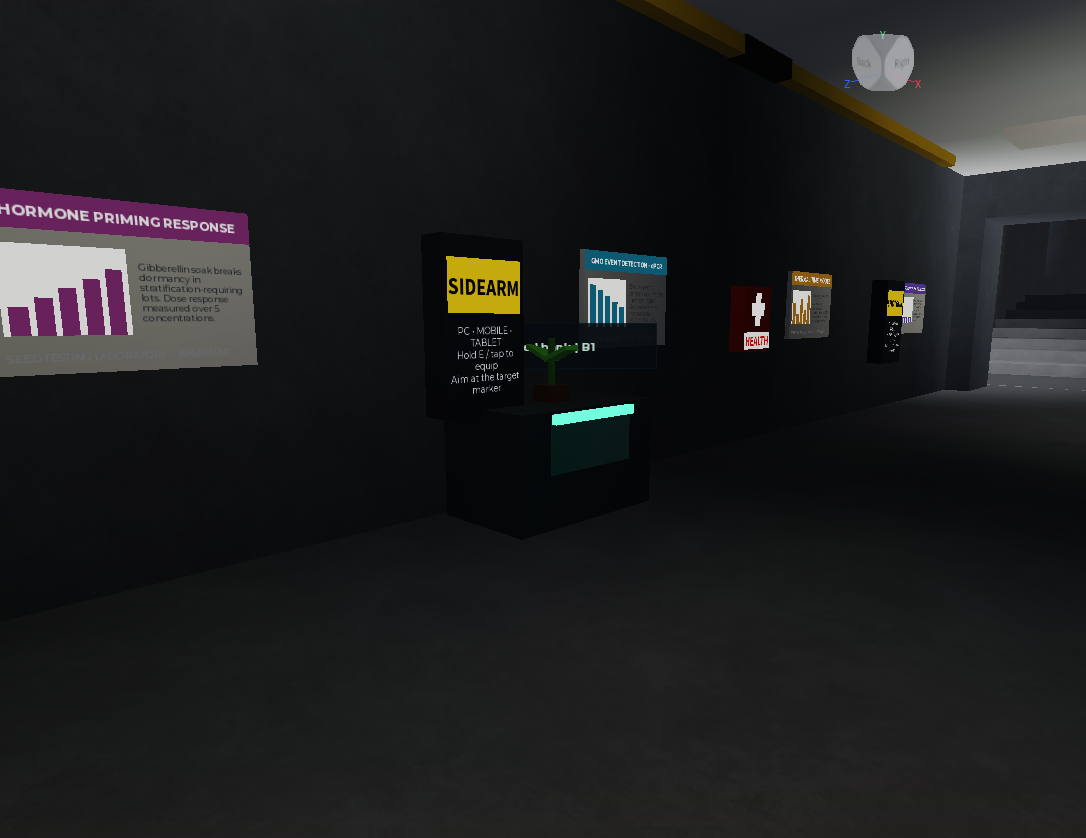
\includegraphics[width=0.92\textwidth]{figures/shots/fig05-seedbank.png}
\caption{The seed bank in the basement. This is the first stop of the
germination assignment and the origin of the mission seedling.}
\end{figure}

\begin{figure}[htbp]\centering
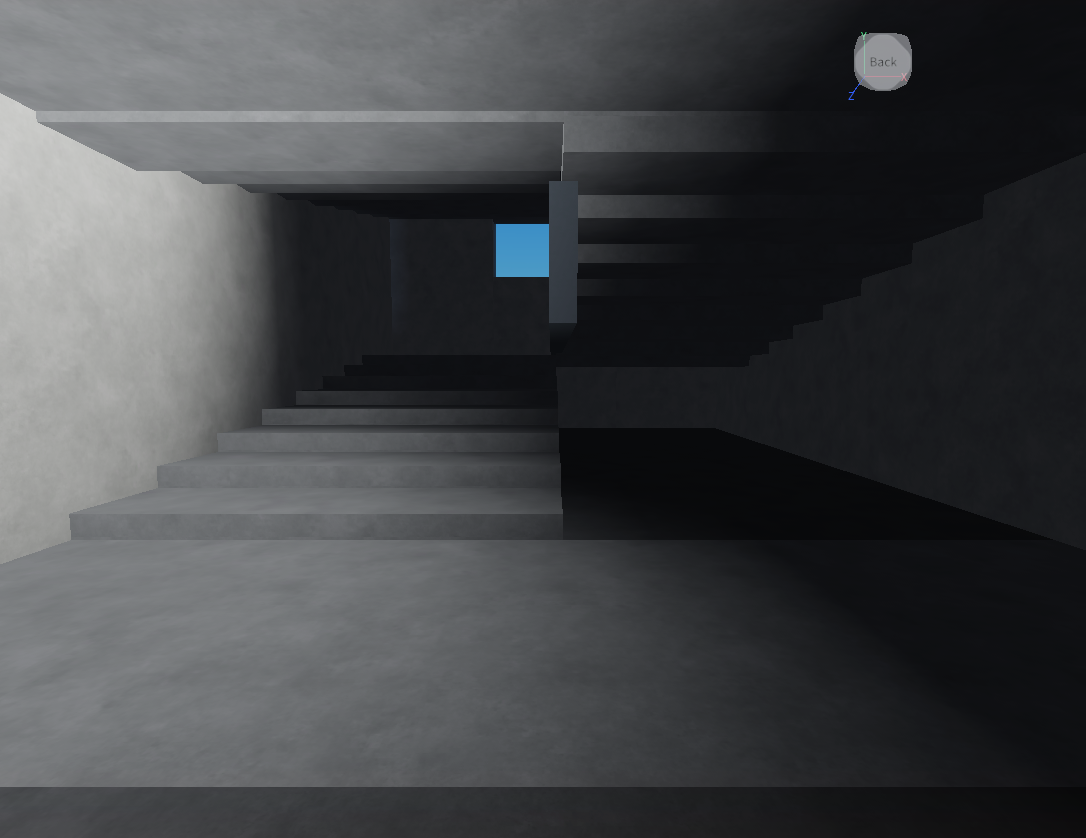
\includegraphics[width=0.92\textwidth]{figures/shots/fig06-basement-stairs.png}
\caption{The basement stair landing, after Revision 5 closed the void beneath
it. Before the repair this landing was a plate with nothing under it and a step
off the edge dropped the player out of the world.}
\end{figure}

\begin{figure}[htbp]\centering
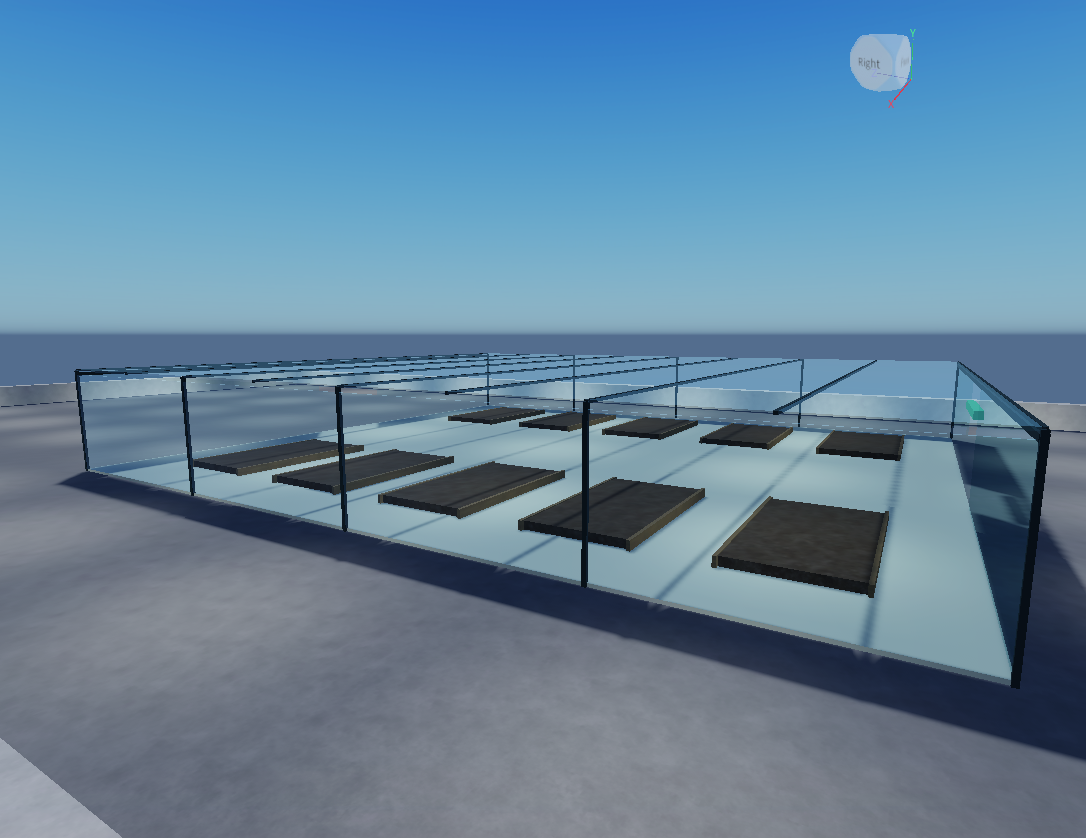
\includegraphics[width=0.92\textwidth]{figures/shots/fig07-greenhouse.png}
\caption{The rooftop greenhouse, the final stop of both assignments. Ten
planting plots sit under the glass; each accepts up to twelve seedlings.}
\end{figure}

\begin{figure}[htbp]\centering
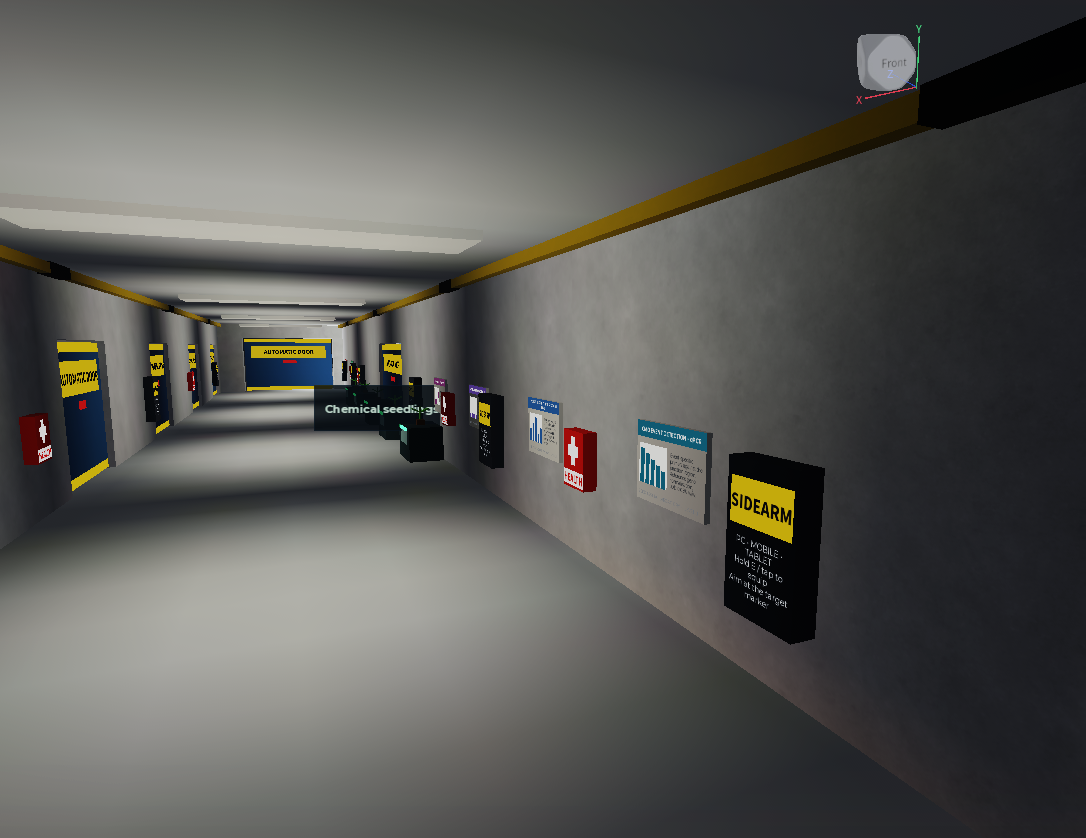
\includegraphics[width=0.92\textwidth]{figures/shots/fig08-fixtures.png}
\caption{Corridor fixtures: an emergency health kit, a weapon cabinet, a
scientific poster, and the yellow gas line running near the ceiling. The gas
line is live ordnance -- a shot into it detonates the section.}
\end{figure}

\begin{figure}[htbp]\centering
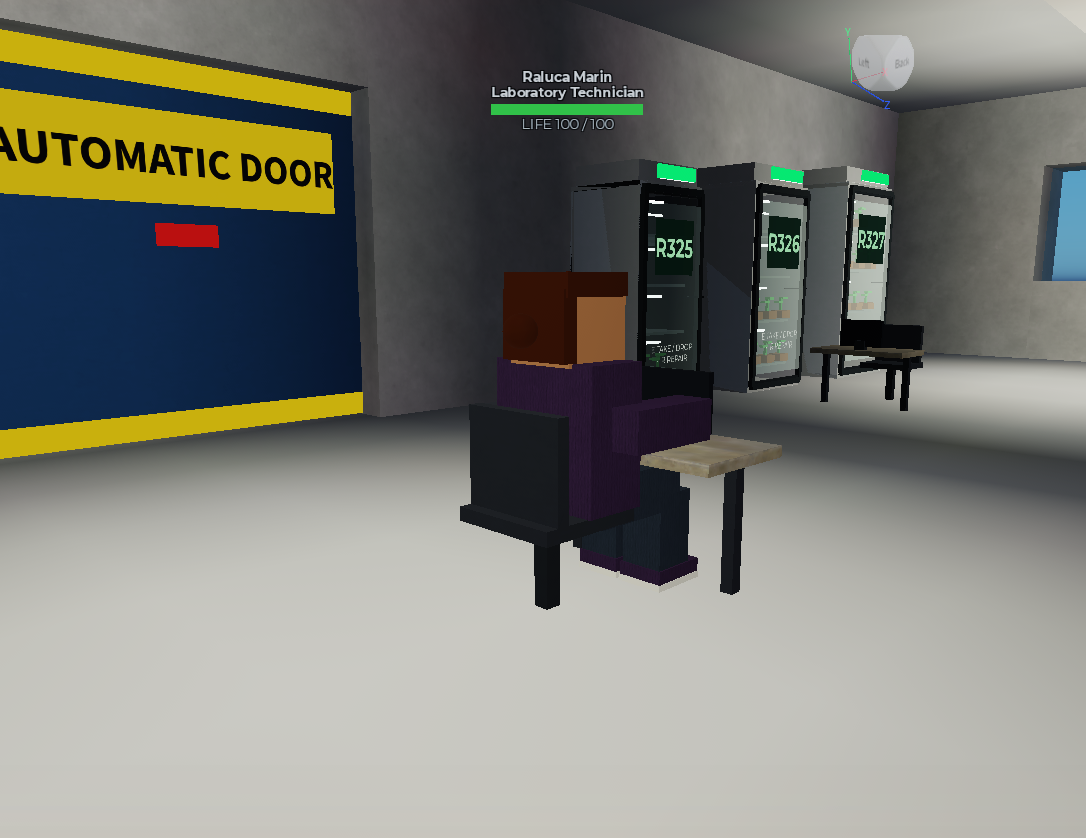
\includegraphics[width=0.92\textwidth]{figures/shots/fig09-seated-worker.png}
\caption{A seated worker at a workstation. Forty-five of the one hundred and
eighty workers are desk staff: they never patrol and never join an ambush, but
they are still targets.}
\end{figure}

\begin{figure}[htbp]\centering
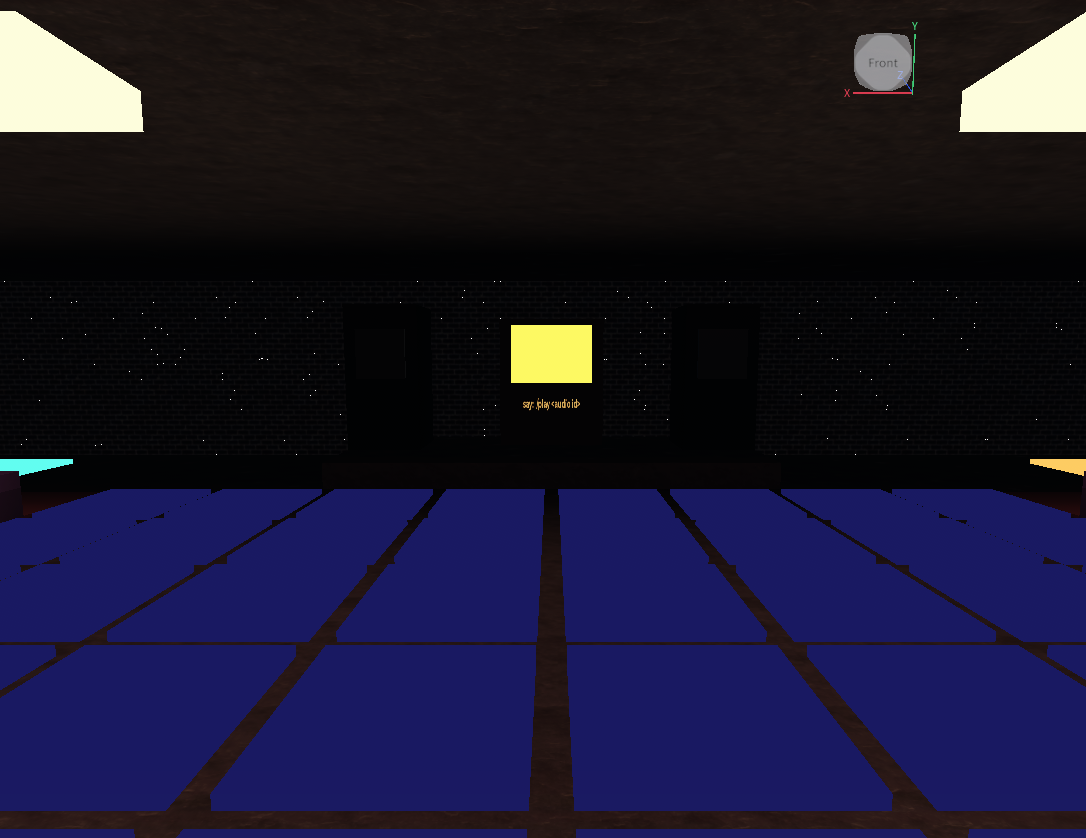
\includegraphics[width=0.92\textwidth]{figures/shots/fig11-lounge.png}
\caption{The hidden lounge, sealed beneath the basement and reached only through
the floor hatch. It has a bar, a stage, a jukebox and a message wall on which
players can post filtered notes.}
\end{figure}

\begin{figure}[htbp]\centering
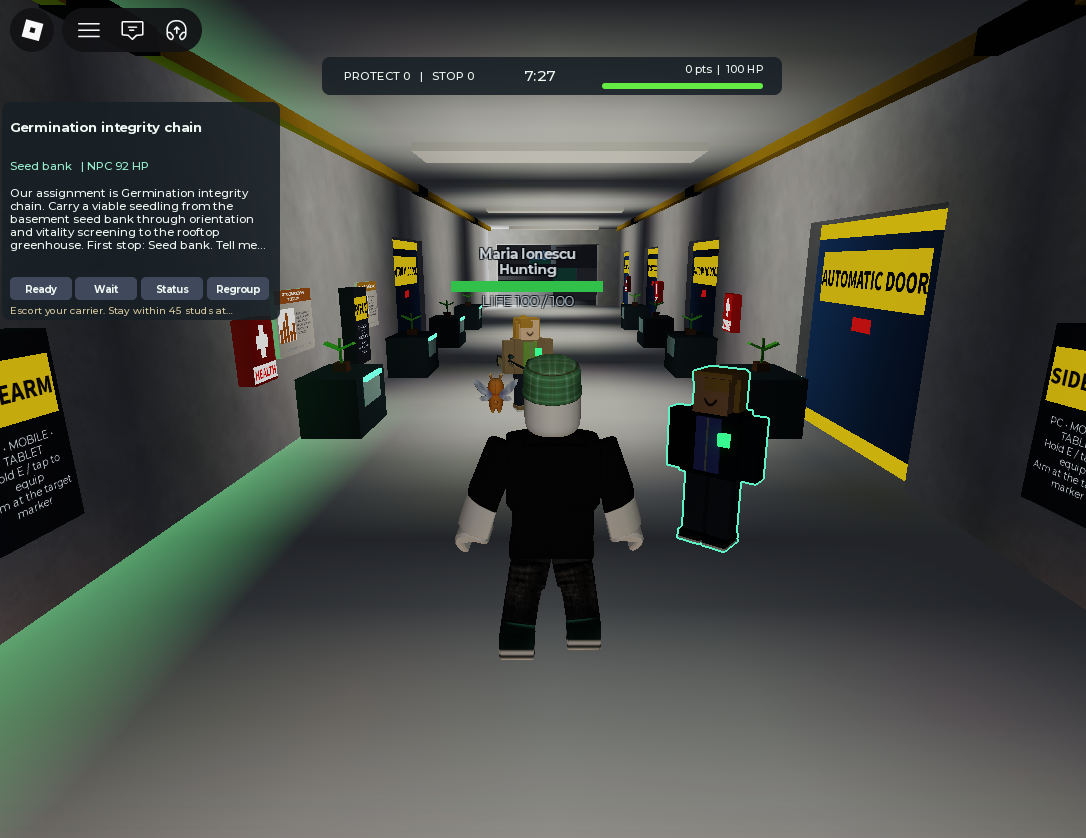
\includegraphics[width=0.92\textwidth]{figures/shots/fig12-hud-ingame.png}
\caption{Gameplay. The mission panel carries the assignment title, the current
stop, the carrier's health and the four carrier commands. The top strip shows
both role scores, the shift clock, points and player health. The green line on
the floor is the mission trail. The worker on the right is a live ambusher --
its billboard reads \emph{Hunting}, the state that tells the patrol system to
stand aside.}
\end{figure}

\begin{figure}[htbp]\centering
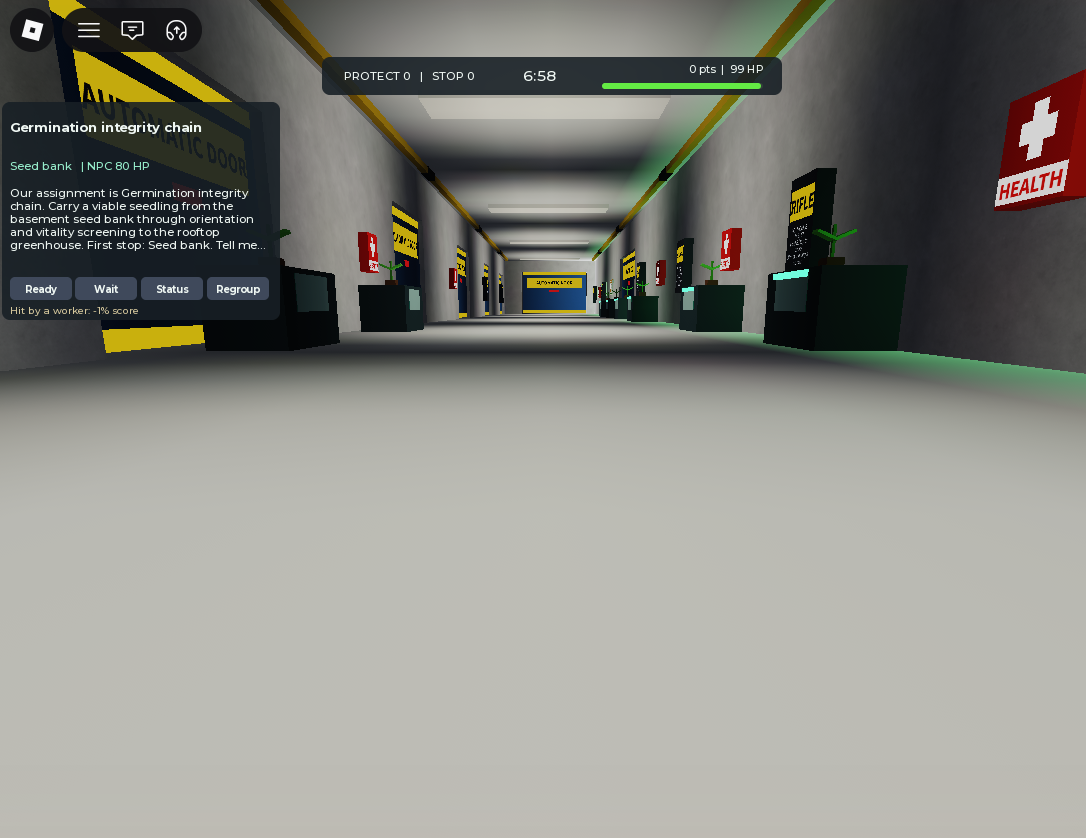
\includegraphics[width=0.92\textwidth,trim=0 430 0 0,clip]{figures/shots/fig13-ambush-standoff.png}
\caption{The same corridor during an ambush, from above and behind. Workers hold
a firing line rather than closing: none comes inside fifteen studs, which is
what makes them aimable.}
\end{figure}

\clearpage
\section{The environment}

\subsection{Scale}
The complex occupies roughly $326 \times 487$ studs in plan and stands 162 studs
from the basement floor to the roof parapet, an envelope of
$x\ -80\ldots246$, $y\ -17\ldots145$, $z\ -141\ldots346$.\ It is built from
61{,}694 parts.\ Nine occupied levels carry between 5{,}831 and 7{,}225 parts
each; the basement is the densest.\

\begin{center}
\begin{tabular}{@{}lr@{}}
\toprule
\textbf{Level} & \textbf{Parts} \\
\midrule
Basement & 7{,}225 \\
Level 1 & 5{,}831 \\
Level 2 & 6{,}140 \\
Level 3 & 5{,}987 \\
Level 4 & 6{,}122 \\
Level 5 & 6{,}005 \\
Level 6 & 6{,}133 \\
Level 7 & 6{,}020 \\
Level 8 & 6{,}123 \\
\bottomrule
\end{tabular}
\end{center}

\subsection{Floor layout}
Every floor is one central corridor with rooms either side.\ The corridor runs
north to south between the two stair towers; the room walls are pierced by
automatic doors that slide up into the header when anyone comes within eleven
studs and hold open for at least three seconds.\ There are 162 such doors.\
The corridor is where the fixtures live: emergency health kits, weapon
cabinets, posters, and the gas line near the ceiling.\

\subsection{Vertical circulation}
Two stair towers, north and south, project beyond the building footprint and
run the full height.\ Each level is served by a landing, a half-landing and two
flights of eight treads.\ There are no working elevators.\ The towers are the
only way between floors, which makes them the natural place to intercept a
carrier and the worst place to be caught by an ambush.\

\subsection{Ground level and the site}
Outside the building the compound holds a perimeter fence with a vehicle gate,
an entrance canopy on posts, parking bays with four cars, two planters, a
flagpole, three glasshouses on the western apron, two trial plots to the east,
and twenty-eight trees.\ The ground plane sits at $y=-8$, between the basement
floor at $-16.25$ and the first floor at $0$.\

\subsection{The rooftop greenhouse}
The roof carries a glazed greenhouse containing ten planting plots.\ Both
assignments end here.\ A plot accepts twelve seedlings before it is full.\ The
greenhouse glass is breakable, and hostile workers will deliberately shoot it
out to open a firing line.\

\subsection{The hidden lounge}
A sealed room sits below the basement, $y\ -49\ldots-30$, reached through a
hatch in the basement floor at $(110, -16, 130)$.\ It contains a bar with
stools, four sofa groups, a stage, a jukebox and a message wall.\ It is out of
play: no mission routes through it and no worker patrols there.\

\section{Characters}

\subsection{The two player roles}
Roles are chosen at one of two kiosks and cannot be changed mid-assignment.\

\begin{center}
\begin{tabular}{@{}p{0.22\textwidth}p{0.70\textwidth}@{}}
\toprule
\textbf{Role} & \textbf{Objective} \\
\midrule
Technician & Escort the research carrier to the rooftop greenhouse. Score for staying within 45 studs at each checkpoint, and for the final planting. Hitting your own carrier cancels your escort rewards. Only a Technician may repair destroyed equipment. \\
Laboratory Technician & Stop the carrier before it plants. Score for bringing it down. \\
\bottomrule
\end{tabular}
\end{center}

Selecting a role assigns one of the two missions immediately.\ There is no
mission menu.\

\subsection{Laboratory workers}
One hundred and eighty workers populate the building.\ They are differentiated
by appearance and name, and forty-five of them are seated desk staff who never
leave their workstation.\ The rest run a shift routine: they respond to
equipment alarms, walk between rooms, and idle when no player is in the room
with them -- an occupancy gate that keeps most of the roster asleep and is the
single largest reason the building runs at all.\

Workers become hostile only through the ambush system.\ At most five are armed
at any moment; when one is put down, a room further along the player's route
releases a replacement.\

\subsection{The research carrier}
The carrier is the mission.\ It is a worker rig that walks the assignment route
under navigation derived from the live map, carries the seedling between
stations, and speaks to its escort through the mission panel.\ It has 100 health
and no weapon.\ If it dies the round is decided in the Laboratory Technician's
favour and a fresh assignment is issued eight seconds later.\

\section{Equipment and fixtures}

\begin{center}
\begin{tabular}{@{}lrp{0.52\textwidth}@{}}
\toprule
\textbf{Fixture} & \textbf{Count} & \textbf{Behaviour} \\
\midrule
Germination chamber & 450 & Destructible. Explodes when shot, killing workers within 17 studs and hurting the player. A Technician restores it by holding R. \\
Research station & 67 & Twenty capabilities, each with an original and two backups, plus ten rooftop plots. Mission stops resolve to a capability, not a specific machine. \\
Automatic door & 162 & Slides open within 11 studs, holds 3 seconds, and can be forced open by an ambush. \\
Emergency health kit & 90 & Restores health, then recharges over 25 seconds. \\
Weapon cabinet & 90 & Dispenses one of the three player weapons. \\
Gas line & 18 & Two runs per floor near the ceiling. Detonates when shot, with a 26-stud blast. \\
Scientific poster & 72 & Takes permanent bullet holes. \\
Luminaire & 333 & Corridor and room lighting. \\
\bottomrule
\end{tabular}
\end{center}

\section{Weapons}
Three weapons are available to players.\ All three cost the shooter one percent
of their score per shot, and a head shot does double damage rather than an
instant kill.\ A worker has 100 health.\

\begin{center}
\begin{tabular}{@{}lrrrrr@{}}
\toprule
\textbf{Weapon} & \textbf{Damage} & \textbf{Pellets} & \textbf{Range} & \textbf{Cooldown} & \textbf{Shots to kill} \\
\midrule
Lab Sidearm & 34 & 1 & 240 & 0.32 s & 3 \\
Lab Shotgun & 12 & 6 & 110 & 0.85 s & 2 \\
Lab Rifle & 55 & 1 & 620 & 0.95 s & 2 \\
\bottomrule
\end{tabular}
\end{center}

The sidearm is the fastest cycling weapon and the only one that stays accurate
while moving.\ The shotgun's 72 damage assumes every pellet connects, which
holds only inside about twenty studs; beyond that it degrades quickly.\ The
rifle is the corridor and stairwell weapon: its 620-stud range covers the full
length of any floor.\

Hostile workers fire a single accurate ray with no spread, once every ten
seconds each, for half a health point per hit.\ Their danger is not the rifle
damage; it is what they do to the room around you.\

\section{Gameplay}

\subsection{The round}
A shift lasts 480 seconds -- eight minutes -- sized from the equipment count and
the mean distance between machines.\ When it ends, destroyed equipment is
repaired, planted seedlings are cleared, bodies are removed and the workers are
stood back up.\

\subsection{Scoring}
\begin{center}
\begin{tabular}{@{}lr@{}}
\toprule
\textbf{Event} & \textbf{Points} \\
\midrule
Protected a research checkpoint (Technician, within 45 studs) & +15 \\
Protected the rooftop planting (Technician) & +60 \\
Stopped the assigned carrier (Laboratory Technician) & +50 \\
Hit by a worker & $-1\%$ of current score \\
Firing any weapon & $-1\%$ of current score \\
\bottomrule
\end{tabular}
\end{center}

The one percent costs are proportional, so they bite hardest when you are
winning.\ A player sitting on a large score loses more per trigger pull than a
player starting out.\

\subsection{Scenario one: the escort, minute by minute}
\begin{center}
\begin{tabular}{@{}p{0.13\textwidth}p{0.79\textwidth}@{}}
\toprule
\textbf{Time} & \textbf{What happens} \\
\midrule
0:00 & Pick the Technician kiosk. The assignment is issued at once and a carrier walks to you. The mission panel names the first stop. \\
0:10 & Press \emph{Ready}. The carrier sets off for the basement seed bank and the green trail appears. \\
0:30 & First stair tower descent. This is the first ambush window: rooms you pass on the way to the stairs wake as you approach. \\
1:00 & Seed bank. The carrier processes for four seconds and takes the seedling. Stay within 45 studs to bank the checkpoint. \\
1:30--4:30 & Four more stops, spread across the basement, Levels 1 and 2. Expect at least one reroute: some stations have no walkable approach and the carrier will divert to a backup with the same capability. \\
5:00 & Long climb to the roof. The stair towers are where an opposing Laboratory Technician will wait, because the carrier cannot avoid them. \\
6:30 & Rooftop greenhouse. The carrier plants the seedling into a plot. Escort bonus awards if you are close. \\
7:00 & Assignment complete. A replacement is issued eight seconds later and the cycle restarts within the same shift. \\
8:00 & Shift ends. Equipment repairs, plots clear, workers stand back up. \\
\bottomrule
\end{tabular}
\end{center}

\subsection{Scenario two: the interception}
\begin{center}
\begin{tabular}{@{}p{0.13\textwidth}p{0.79\textwidth}@{}}
\toprule
\textbf{Time} & \textbf{What happens} \\
\midrule
0:00 & Pick the Laboratory Technician kiosk. You are assigned the cold-chain audit and a carrier of your own. \\
0:20 & Collect a rifle from a corridor cabinet. The rifle, not the shotgun: you will be shooting down corridors and stairwells. \\
1:00 & Locate the carrier. Its destination floor is on the mission panel, so you can move to the stairwell it must use rather than chase it. \\
2:00 & Take the stairwell. A carrier in a flight cannot leave it and cannot shoot back. \\
2:30 & Sustained fire brings it down in about 25 seconds unopposed; far less with the ambush helping, since half of every ambush targets the carrier. \\
3:00 & +50 points. A replacement carrier is issued, and you reposition for the next one. \\
\bottomrule
\end{tabular}
\end{center}

\section{Tactics worth knowing}
These are consequences of how the systems are built, verified by measurement.\
They are legitimate play, not defects, but they are not obvious.\

\begin{enumerate}
\item \textbf{Let the ambush kill the carrier for you.}\ Half of every ambush is
      assigned to the carrier when it wakes.\ As a Laboratory Technician you
      often do not need to fire at all -- shadow the carrier, stay out of the
      standoff line, and let the building do the work.\
\item \textbf{As a Technician, pull the ambush off the carrier.}\ Hostiles that
      are not carrier hunters switch to whoever is closest.\ Standing on the far
      side of the corridor from your carrier drags the other half of the roster
      onto you, which is survivable at half a point per hit.\
\item \textbf{Never fight next to a gas line.}\ Hostiles deliberately shoot
      pipes and machines near you.\ The blast radius is 26 studs for a pipe and
      17 for a machine, and both hurt you far more than a rifle round.\ Fight in
      the middle of the corridor, not against the wall where the fixtures are.\
\item \textbf{Weapon cost is proportional.}\ At 1\% of score per shot, a missed
      burst late in a round costs more than the same burst early.\ Once you are
      ahead, stop firing and escort.\
\item \textbf{Head shots are worth aiming for, but not decisive.}\ They double
      damage; they no longer kill outright.\ A rifle head shot still takes a
      worker down in one, a sidearm head shot does not.\
\item \textbf{Emergency kits recharge, so corridors are safe ground.}\ Ninety
      kits on a 25-second cycle means sustained hostile fire is survivable
      indefinitely if you keep moving between them.\
\item \textbf{Break the line of sight rather than the distance.}\ Hostiles hold
      at twenty studs and shoot accurately, but they will not close.\ Stepping
      into a room and letting the door shut ends the engagement outright.\
\item \textbf{Repair is a scoring move for Technicians.}\ Destroyed equipment
      removes a station from the mission pool and can force a reroute.\ Repairing
      it near a carrier's next stop shortens the route.\
\item \textbf{Stairwells favour the interceptor.}\ A carrier on a flight follows
      the treads and cannot deviate, which makes its position predictable for
      several seconds.\
\item \textbf{The rooftop is the last chance, not the best one.}\ Hostiles will
      shoot out the greenhouse glass to reach you, so cover there is temporary.\
\end{enumerate}

\chapter{Revision 5: coordinate repair, navigation, and the hostile ambush}

\section{Summary}
Revision 5 began as a correction to Revision 4 and became a rebuild of three
subsystems.\ It reverses a geometry migration that had been applied to the wrong
object, closes a fall-through hazard in the basement, replaces the research
carrier's hardcoded route table with navigation derived from the live map,
reduces the ten selectable scenarios to two role-bound assignments, and adds a
hostile ambush system in place of the previous passive opposition.\

All work in this chapter was applied to the live place through the Studio
bridge and verified by numeric scene queries and instrumented play sessions
rather than by observation alone.\

\section{The coordinate fault and its repair}

\subsection{Diagnosis}
Revision 4 concluded that \texttt{Laboratory\_Complex} had shifted and that the
lounge should be moved to follow it.\ It inferred the displacement
$(-25.142857,\ -23.25,\ +91.285714)$ studs and applied it to
\texttt{Workspace.Lounge} and \texttt{Workspace.LoungeHatch}, a total of 169
parts.\

The vector was correct.\ The object was not.\ Ground truth was recovered from
\texttt{D:\textbackslash game\textbackslash 4\textbackslash Export.gltf},
exported on 11 September 2026, which stores the authored node translations:

\begin{center}
\begin{tabular}{@{}lll@{}}
\toprule
\textbf{Node} & \textbf{Authored} & \textbf{Live before repair} \\
\midrule
\texttt{Laboratory\_Complex/Roof\_1} & 82.2857,\ 129.375,\ 133.7143 & 57.1429,\ 106.125,\ 225.0000 \\
\texttt{LoungeHatch} & 110,\ $-15.9$,\ 130 & 84.857,\ $-39.150$,\ 221.286 \\
\texttt{HatchRim} & 110,\ $-16$,\ 130 & 110,\ $-16$,\ 130 \\
\texttt{Lounge/Floor} & 80,\ $-49$,\ 130 & 80,\ $-72.25$,\ 221.286 \\
\texttt{LabSpawn} & 32.143,\ 1,\ 11.571 & 32.143,\ $-0.1$,\ 11.571 \\
\bottomrule
\end{tabular}
\end{center}

\texttt{HatchRim}, the three spawn markers and
\texttt{LaboratoryFoundationGround} had not moved.\ Only the laboratory had.\
Because the ground plane remained at $y=-8$ while the first floor sank to
$-23.25$, the ground plane sat 15.25 studs above the first floor and intersected
Levels 1 and 2.\ That is the reported gap in the building and the exterior.\

Revision 4's partial migration made the fault worse: the lounge followed the
displaced building while the hatch's own rim did not, leaving a hatch and its
rim 95 studs apart.\

A further confirmation is available in Revision 4's own code.\ The constant
\texttt{BASE\_ROOF} in \texttt{LabSpatial} is
\texttt{CFrame.new(82.28571428571429,\ 129.375,\ 133.71428571428572)}, which is
exactly the authored roof position.\ The frame that module composed was
therefore identity with respect to the authored datum, not with respect to the
displaced one.\

\subsection{Repair and verification}
Two rigid moves were applied, each guarded before execution:

\begin{enumerate}
\item \texttt{Lounge} and \texttt{LoungeHatch}, 169 parts, by
      $(+25.142857,\ +23.25,\ -91.285714)$.\ The move was performed only
      because the inverse placed \texttt{LoungeHatch} within 0.1 studs of
      \texttt{HatchRim}; otherwise the operation refused and changed nothing.\
\item \texttt{Laboratory\_Complex}, by the delta that returns \texttt{Roof\_1}
      to its exported position, as a single \texttt{PivotTo}.\
\end{enumerate}

\begin{center}
\begin{tabular}{@{}ll@{}}
\toprule
\textbf{Check} & \textbf{Result after repair} \\
\midrule
\texttt{Roof\_1} & 82.2857,\ 129.375,\ 133.7143, the exported value \\
Level\_1 slab top & 0.000 \\
Basement slab top & $-16.250$ \\
Ground plane & $-8.000$, correctly between the two \\
Research stations on a real slab & 67 of 67, none in mid-air \\
Laboratory spawns & all three resting on \texttt{FloorSlab\_1} \\
Building parts inside the lounge volume & 1963 $\rightarrow$ \textbf{0} \\
Part counts & 61513 / 168 / 4 / $1\times6$, unchanged \\
\texttt{LabSpatial.frame()} translation & \textbf{0.0000} \\
\bottomrule
\end{tabular}
\end{center}

The final row is the operative one.\ With the map restored to its authored
datum, Revision 4's entire coordinate layer evaluates to identity and is inert.\
It was therefore removed rather than unpicked:
\texttt{ReplicatedStorage.LabSpatial} was moved to
\texttt{ServerStorage.LabSpatial\_RETIRED\_revision4}, and all thirty
\texttt{Spatial.*} call sites were reverted by rebuilding the affected scripts
from the pre-Revision-4 baseline.\

\subsection{Correction to the Revision 4 record}
The Revision 4 entry in \texttt{ServerStorage.GameDocumentation} states ``The
building itself was not moved back'' and ``Do not move the lounge twice''.\ Both
are now false and both would mislead a later reader.\ A correction notice was
prepended to that module, and the \texttt{LabFrameAligned} marker on
\texttt{Workspace.Lounge} was cleared.\

\section{Basement stair-tower void}
Both stair towers sit outside the basement slab: \texttt{StairTower\_North} at
$z=-6.4$ and \texttt{StairTower\_South} at $z=273.9$, while
\texttt{BasementSlab} spans $z=0$ to $267.4$.\ Each \texttt{Landing\_L-1} was
therefore a plate 0.75 studs thick with nothing beneath it, and a player
stepping off its edge fell into the void.\ This is the blue area reported at the
foot of the basement stairs; the colour is the skybox seen through the gap.\

A \texttt{TowerBaseSlab} was added under each tower at the basement datum,
matching the basement slab's material and colour.\ A sweep of 6073 sample
points across the basement floor and both tower footprints subsequently found
zero unsupported points, and every edge of both basement landings resolves onto
either \texttt{TowerBaseSlab} or \texttt{BasementSlab}.\

\section{Carrier navigation and physical movement}

\subsection{The fault}
The research carrier walked through walls, equipment and floors.\ The cause was
structural rather than incidental.\ \texttt{routePoints} returned a hardcoded
polyline: corridor lane $x=78$, stair lane $x=68.7857$, tower mouth $z=-6$, and
per-tread offsets of the form $-15.267857-(i-1)\times 4.821428$.\ The walk loop
then advanced the rig with \texttt{PivotTo}, testing only for player proximity
so as not to shove them.\ No test of geometry existed anywhere in the path, so
walls were not merely passable, they were absent from the model.\

\subsection{GWAPNavigation}
Routing was replaced by \texttt{ReplicatedStorage.GWAPNavigation}, which reads
the map as it exists at the moment of the request.\ Levels come from the actual
\texttt{FloorSlab} and \texttt{BasementSlab} parts; flights come from the named
tread parts inside each \texttt{StairTower}; and the approach point for a
station is recomputed from that station's live bounds, filtered by a ground
test, a line-of-sight test and a body-box clearance test.\ No coordinate is
stored, so relocated equipment and re-packed rooms cannot strand a carrier.\

The walk loop was made physical.\ Because the rig is anchored and driven by
\texttt{PivotTo}, which bypasses the physics solver, each step is swept against
the world by hand: a blocked step is never applied, and an applied step is
followed onto the surface beneath it so the carrier can neither sink through a
floor nor walk on air.\ A persistent obstruction recomputes the route rather
than waiting out the mission clock.\

\subsection{Defects found during integration}
Four faults were introduced or exposed while wiring this in, and are recorded
because each is a general trap rather than a local slip.\

\begin{enumerate}
\item \textbf{Ground follow fought a deliberate climb.}\ A waypoint 0.82 studs
      directly above the carrier, with zero horizontal component, could never be
      reached: the surface snap reset the height on every frame.\ The loop span
      indefinitely with no error and no message.\ The snap now applies only when
      the step carries horizontal travel.\
\item \textbf{Degenerate waypoints.}\ Two landing points measured against
      different surfaces produced purely vertical hops, which are unreachable
      for a walker.\ \texttt{GWAPNavigation} folds them into the following
      point.\
\item \textbf{Unbounded waypoint wait.}\ A single unreachable waypoint could
      hold a mission indefinitely.\ A per-waypoint deadline now abandons it, and
      three consecutive failures recompute the route.\
\item \textbf{Sticky target bypassed the reachability test.}\ Once
      \texttt{a.target} was set, the first branch of the selection expression
      returned it without consulting the reachability predicate, so an
      unreachable station was proposed forever.\
\end{enumerate}

\subsection{Measured result}
A full instrumented run, sampled every 70 milliseconds:

\begin{center}
\begin{tabular}{@{}ll@{}}
\toprule
Distance walked & approximately 1190 studs, basement to roof \\
Wall penetrations & \textbf{0} \\
Airborne frames & \textbf{0} \\
Automatic reroutes & 2, around unreachable equipment \\
Mission stages completed & 4 of 4 \\
\bottomrule
\end{tabular}
\end{center}

\section{Role-bound assignments}
The ten selectable scenarios were replaced by two, one per role, each a
six-stop run spanning basement, intermediate floors and the rooftop greenhouse:

\begin{center}
\begin{tabular}{@{}p{0.28\textwidth}p{0.62\textwidth}@{}}
\toprule
\textbf{Assignment} & \textbf{Route} \\
\midrule
Germination integrity chain & Seed bank, Incubator, Clinostat, Orientation scanner, Vitality scanner, rooftop plot \\
Cold-chain contamination audit & Cryo-freezer, Wet lab, Symbiosis incubator, Chemical seedlings, Porometer, rooftop plot \\
\bottomrule
\end{tabular}
\end{center}

Every stop is a station capability with three instances in the map, one original
and two backups, so a destroyed or unreachable stop reroutes to an equivalent
rather than stalling the run.\

Selection was removed entirely.\ Setting \texttt{LabRole} assigns one of the two
immediately; the HUD's job button, scenario menu, list and random-assignment
control were deleted; and the server now refuses a \texttt{choose} action
arriving from a client, since after this change it can only be a stale HUD or a
crafted packet.\ Because nothing can be chosen, \texttt{finish()} issues the
next assignment eight seconds after a mission ends.\

\section{Hostile ambush system}
The previous opposition fired once every 2.5 seconds, only when a single player
was present, and then applied a random spread of $\pm2.5$ studs, so it usually
missed and never left its room.\ It was replaced.\

\begin{center}
\begin{tabular}{@{}p{0.30\textwidth}p{0.60\textwidth}@{}}
\toprule
\textbf{Behaviour} & \textbf{Mechanism} \\
\midrule
Emerge from rooms & rooms within 58 studs release up to two workers; the door is held open for nine seconds through a \texttt{ForceOpen} attribute honoured by \texttt{bindAutoDoor} \\
Stairs and greenhouse & pursuit is position-based rather than room-based, so workers follow onto the towers and the roof \\
Accurate fire & a single ray to the target with no spread \\
Hazards & a proportion of shots target a gas pipe or a live machine beside the player \\
Greenhouse glass & a shot blocked by greenhouse glass shatters it, clearing the line for the next \\
Carrier as target & half of each ambush is assigned to the carrier when it wakes \\
Bounded cost & a hard roster cap, replenished from later rooms as workers are put down \\
\bottomrule
\end{tabular}
\end{center}

\subsection{Interaction with the patrol system}
Hostile workers initially did not move at all.\ The existing patrol logic in
\texttt{LabEquipment} was calling \texttt{PivotTo} on the same rigs; two systems
driving one rig cancel each other out.\ The patrol now yields for as long as
\texttt{GWAPHostile} is set.\ A second cause followed: a three-direction wall
slide could not negotiate a laboratory dense with benches, and the sweep was
correctly refusing to pass through an incubator.\ Steering was widened to eight
headings with a real path solve when a worker is stuck, throttled to at most one
solve per second across the whole roster.\ Seated desk staff are excluded, since
they have no walking pose.\

\section{Damage model corrections}

\subsection{Fractional damage}
The rate limiter returned a fraction of the requested damage.\ With several
shooters sharing one budget, each landed shot was scaled to roughly half a
point, so a hit did not read as a hit.\ The limiter now governs how often a
shot may hurt, never how much: a shot either lands for its full value or is
spent as a near miss.\

A constraint follows from this and is recorded because it is not obvious: under
all-or-nothing accounting the cap must be at least the size of one hit, or no
shot can ever afford to land.\ One hit per second is therefore the fastest
possible cadence, and survival time is set by hit size rather than by the cap.\

\subsection{Universal one-shot kill}
Every weapon killed a full-health worker in a single shot.\ The cause was not a
damage value.\ It was the line

\begin{center}
\texttt{tool:SetAttribute("BlasterInstantHeadshot", style.pcOnly == true)}
\end{center}

Each of the three player weapons sets \texttt{pcOnly = true}, so instant-headshot
was enabled on all of them.\ Whenever a ray cleared the worker's collision hull
and caught the head, the shot killed outright regardless of the weapon.\
Reducing the shotgun's pellet damage in an earlier pass could not address this,
because the lethality never came from the damage figure.\

A head shot now doubles damage instead of ending the engagement, in both firing
paths.\ This closes every thousand-damage route through a gun; the remaining
thousand-damage calls are the equipment and gas-pipe explosions, which are
intended to be lethal.\ Verified through the live \texttt{BlasterHitBridge}
against a full-health worker:

\begin{center}
\begin{tabular}{@{}lll@{}}
\toprule
\textbf{Weapon} & \textbf{Damage} & \textbf{Shots to kill} \\
\midrule
Lab Sidearm & 34 & 3 \\
Lab Shotgun & $6\times12$ & 2 \\
Lab Rifle & 55 & 2 \\
\bottomrule
\end{tabular}
\end{center}

The bridge itself was never at fault.\ An isolated invocation carrying 34 damage
took a worker from 100 to exactly 66, which is the measurement that eliminated
\texttt{damageWorkerBot} and the weapon table and identified the tool attribute.\

\subsection{Standoff}
Workers closed to six studs and formed a press the player could not aim through.
They now hold a firing line: a worker closes only to \texttt{STANDOFF}, gives
ground if it ends up inside \texttt{STANDOFF\_MIN}, and applies a separation
push away from every other hostile within \texttt{SPACING} on every tick.\
Applying separation only once a worker had stopped, which was the first attempt,
left those still closing to pile into those that had halted.\

A wider line of 24 and 17 studs was tried first and held the workers so far back
that corridor equipment broke line of sight and nothing landed at all across 28
seconds of observation.\ The values below keep clear room to aim while leaving
the workers in sight of the player.\

\section{Constants reference}
\begin{center}
\begin{tabular}{@{}lll@{}}
\toprule
\textbf{Constant} & \textbf{Value} & \textbf{Meaning} \\
\midrule
\texttt{HOSTILE\_CAP} & 5 & armed workers active at once \\
\texttt{PER\_ROOM} & 2 & released from any one room \\
\texttt{RELEASE\_RADIUS} & 58 & distance at which a room wakes \\
\texttt{SHOT\_INTERVAL} & 10 s & one shot per worker \\
\texttt{HOSTILE\_DAMAGE} & 0.5 & absolute health points per landed hit \\
\texttt{INCOMING\_CAP} & 5 & combined limit, above hit size so all shots land \\
\texttt{CARRIER\_DAMAGE} & 4 & per landed hit on the carrier \\
\texttt{CARRIER\_INCOMING\_CAP} & 4 & one hit per second, roughly 25 s unaided \\
\texttt{CARRIER\_HUNTER\_SHARE} & 0.5 & fraction of an ambush assigned to the carrier \\
\texttt{HAZARD\_CHANCE} & 0.08 & odds a shot targets a pipe or machine \\
\texttt{STANDOFF} & 20 & distance held from the target \\
\texttt{STANDOFF\_MIN} & 15 & closer than this, the worker gives ground \\
\texttt{SPACING} & 9 & minimum separation between hostiles \\
\bottomrule
\end{tabular}
\end{center}

Measured with these values: recorded hit sizes of 0.5 throughout, 15 hits across
35 seconds from four to five workers, player health 100 to 94.5, closest
approach 13 studs, typical engagement distance 44 studs, no script errors.\

\section{Open items}
\begin{enumerate}
\item \textbf{Nine unroutable stations.}\ Nine of the 67 research stations have
      no walkable approach route.\ All are originals positioned at $x=67$, hard
      against the corridor's western wall.\ Missions reroute to backups
      automatically, so play is unaffected, but those nine are decoration until
      they are moved clear of the wall.\
\item \textbf{Cause of the original displacement is unknown.}\ If a generator
      rebuild writes the laboratory at a different origin, the fault recurs.\
      Before any full regeneration, \texttt{Roof\_1} should be checked against
      $(82.2857,\ 129.375,\ 133.7143)$.\
\item \textbf{Two runtime copies.}\ The weapon table and several helpers exist
      both in the installed scripts and in the generator's embedded payload.\
      The corrections in this chapter were applied to the installed scripts; a
      full regeneration would restore the previous values.\
\end{enumerate}

\chapter{Revision 4: live repairs and current handover}
\section{Authority and chronology}
This chapter supersedes the pre-revision findings wherever a repair is explicitly recorded here.\allowbreak{} The baseline inventory was captured from Studio version 70; the owner reopened version 72 and all 29 source fingerprints matched that baseline before modification.\allowbreak{} The owner then explicitly authorized conservative live repairs and documentation inside source comments.\allowbreak{} The changes below were installed through Studio MCP in Edit mode and exercised in fresh Play sessions on 13 September 2026.\allowbreak{} No publishing action was performed.\allowbreak{} The exported RBXL remains the original evidence, not a post-repair save.\allowbreak{}

\section{What was actually changed}
C01, stale coordinate metadata: the laboratory had moved by approximately (-25.\allowbreak{}142857, -23.\allowbreak{}25, 91.\allowbreak{}285714) studs while navigation still used generator coordinates.\allowbreak{} LabSpatial derives a frame from the existing Roof\_\allowbreak{}1 landmark and its original generator CFrame.\allowbreak{} World construction, station backups, mission stairs, rendezvous, legacy repair routes, room lookup, worker patrol destinations, room smoke and door ventilation now translate between laboratory-local coordinates and world coordinates explicitly.\allowbreak{} Each of the 67 station approaches has an ApproachPoint attachment.\allowbreak{} Its world position follows subsequent station movement; ApproachLocal preserves the migration input.\allowbreak{} The building itself was not moved back.\allowbreak{}

A second scene mismatch was found by sweeping a carrier-sized box along the corrected route: Lounge.\allowbreak{}Wall\_\allowbreak{}N intersected the basement stair exit.\allowbreak{} The laboratory had moved but the lounge and its hatch had not.\allowbreak{} All 169 associated BaseParts were transformed once by the same laboratory frame.\allowbreak{} Original CFrames are retained in the live rollback folder.\allowbreak{} This is a scene migration, not a repeating runtime translation.\allowbreak{} Future whole-world moves must include the lounge, hatch and laboratory together.\allowbreak{}

C02, incorrect installer payload: the loose GWAPWorld.\allowbreak{}lua and old InstallGWAP.\allowbreak{}lua contained mission-server code under the world-module name.\allowbreak{} The corrected root module is the verified world implementation.\allowbreak{} The root installer is regenerated from the final source set, including LabSpatial and changed legacy dependencies.\allowbreak{} It is a small local-HTTP preflight loader, with complete source payloads in release/\allowbreak{}.\allowbreak{} Each payload is length/\allowbreak{}checksum verified and compiled before mutation.\allowbreak{} A monolithic payload would exceed Studio's 200,000-byte Script.\allowbreak{}Source limit.\allowbreak{} Serve the documentation folder on localhost port 8766; no external hosting is required.\allowbreak{} Historical copies under code/\allowbreak{}workspace remain unchanged and are explicitly pre-revision evidence.\allowbreak{} Do not confuse those historical files with the corrected root release.\allowbreak{} The large generator is not rebuilt or executed by this revision.\allowbreak{}

R01, research repair authority: the server now requires a living Technician, workspace membership, no BlastRemoved flag, an exploded target, proximity within 14 studs and an unobstructed ray from the player's head to the equipment.\allowbreak{} UI prompt visibility alone no longer authorizes repair.\allowbreak{} HoldDuration remains an interface duration; this revision does not certify resistance to forged hold timing.\allowbreak{} That is a remaining security-hardening task, not a claim of complete exploit resistance.\allowbreak{}

R02, carrier collision: the existing anchored carrier route movement now performs a 2.\allowbreak{}4 by 4.\allowbreak{}4 by 2.\allowbreak{}4 stud swept query before each short movement step.\allowbreak{} A solid obstacle stops movement, extends the mission deadline and produces an explanatory dialogue at most once per ten seconds.\allowbreak{} Clearing the obstacle resumes travel.\allowbreak{} Arbitrary obstacle detours are not promised; Wait and Regroup remain the recovery controls.\allowbreak{} Player movement, camera, mouse aiming, mobile aiming, gun recoil and input bindings are preserved.\allowbreak{}

R03, solo eligibility: only living active NPCs in Workspace enter the armed selection.\allowbreak{} Stored carriers and knocked-out/\allowbreak{}dead workers are excluded.\allowbreak{} The armed count is floor(eligible count * 0.\allowbreak{}2).\allowbreak{} Eligibility is reconciled when population state changes and on a five-second bounded check; already selected gun instances are reused.\allowbreak{} The original inventory mesh specifications are unchanged.\allowbreak{}

R07, shared lounge notes: player-authored note text passes through TextService.\allowbreak{}FilterStringAsync and GetNonChatStringForBroadcastAsync before broadcast.\allowbreak{} Failed filtering produces no shared note.\allowbreak{} A three-second per-player cooldown bounds requests.\allowbreak{} Departure clears note cooldown and skip-vote state.\allowbreak{} Published-service filtering behavior is not certified by a local Studio session; the fail-closed source path is the evidence for this change.\allowbreak{}

HUD and allocation fixes: the carrier's health is folded into the existing mission target line, and its duplicate overhead billboards are hidden.\allowbreak{} GWAPNPC.\allowbreak{}say retains dialogue attributes but no longer creates a server-enabled MissionSpeech billboard; this removes the observed flash before client suppression and the redundant GUI instances.\allowbreak{} Other targeted NPC billboards are suppressed near the top HUD.\allowbreak{} Existing compact layout and original weapon controls are retained.\allowbreak{} Pool reactivation no longer installs duplicate billboard watchers.\allowbreak{} Route nodes are sorted once until ChildAdded or ChildRemoved invalidates the cache, allowing incremental replication.\allowbreak{} Terminal missions immediately destroy their route nodes.\allowbreak{} These are bounded allocation reductions; no invented megabyte saving or sixty-player performance claim is made.\allowbreak{}

\section{Fresh verification results}
V4-01: all seven initial changed/\allowbreak{}new source files compiled in Studio before installation.\allowbreak{} A fresh Play session reported no server or client MessageError entries at the inspected checkpoints.\allowbreak{}

V4-02: Incubator approach migrated from (78, 3.\allowbreak{}25, 49) to approximately (52.\allowbreak{}857147, -20, 140.\allowbreak{}285706), adjacent to its actual body at (41.\allowbreak{}857147, -21.\allowbreak{}75, 140.\allowbreak{}285706).\allowbreak{} The initial companion appeared 8.\allowbreak{}0163 studs from the player.\allowbreak{} Four unused carriers stayed in ServerStorage.\allowbreak{} Solo count was 36 armed among 181 active eligible NPCs.\allowbreak{}

V4-03: scenario 1 completed seed bank, instrument and rooftop planting in the corrected scene.\allowbreak{} Plot 1 gained one plant, score increased from 0 to 90 and route-folder count returned to zero.\allowbreak{} Scenario 2 then completed and the cumulative score became 180.\allowbreak{} A test-only server helper kept the owner six studs beside the moving carrier and restored health; it did not shoot, modify points, advance stages or move the carrier.\allowbreak{} This verifies mission execution and clean rewards, not human stair-navigation skill or multiplayer load.\allowbreak{} Helpers existed only in Play and were discarded on Stop.\allowbreak{}

V4-04: equivalent-station selection chose Incubator - Backup 1 on floor 0 after primary destruction, then Incubator - Backup 2 on floor 1 after the first backup was made unavailable.\allowbreak{} The controlled selection test restored station flags afterward.\allowbreak{} Full mission fallback across every capability remains a broader regression target.\allowbreak{}

V4-05: a temporary solid obstacle inserted into a live carrier route produced zero movement over a half-second stopped sample.\allowbreak{} After removal, the carrier moved 9.\allowbreak{}9987 studs in approximately half a second with owner WalkSpeed 20.\allowbreak{} The obstruction dialogue appeared.\allowbreak{} No player movement settings were changed by the carrier implementation.\allowbreak{}

V4-06: a controlled exploded wall section removed a health station, gun fixture, poster and research-equipment fixture from Workspace.\allowbreak{} A fixture outside the section stayed present and unmarked.\allowbreak{} All test geometry was cleaned up.\allowbreak{} Existing actual-wall selection and quarantine behavior are retained.\allowbreak{}

V4-08: in a fresh final-source Play session, holding R within six studs restored an exploded Incubator for the Technician role.\allowbreak{} Repeating the same interaction as Laboratory Technician left the target destroyed, as required.\allowbreak{} No server errors were reported.\allowbreak{} An earlier attempt at the outer edge of prompt range did not activate; the closer prompt interaction is the successful observation.\allowbreak{}

V4-07: a 705 by 338 client viewport loaded without client errors.\allowbreak{} Visual inspection found a carrier overhead-bar overlap with the top strip, leading to the final health-in-panel change.\allowbreak{} The final UI recheck is recorded in VERIFICATION.\allowbreak{}md.\allowbreak{} The accepted Blaster and BlasterController executable bodies are unchanged; their final differences are documentation comments only.\allowbreak{} Earlier 90-frame idle and walking grip measurements remain historical tests, not newly repeated measurements.\allowbreak{}

\section{Remaining boundaries and next engineering work}
Wall destruction remains persistent within the current server session: fixtures are quarantined and walls are not recreated automatically at a round change.\allowbreak{} A future restoration system must restore both the wall and its original fixture parent, tags, prompt state and callbacks in a single lifecycle contract.\allowbreak{} Reparenting fixtures alone would restore floating equipment.\allowbreak{} This behavior is disclosed rather than silently introducing a new world-reset policy.\allowbreak{}

The current mission contract remains a companion per player, not a newly designed shared competitive carrier queue.\allowbreak{} There is no certified sixty-player load test, no persistent real-science dataset and no exhaustively tested gamepad support.\allowbreak{} The ten scenarios remain research-inspired workflows.\allowbreak{} Real GWAP data validation and exports are future engineering specifications in the scenario chapters.\allowbreak{}

\section{How another AI should modify this revision}
Start by comparing the open place ID and source hashes with the release manifest.\allowbreak{} Preserve a local and server-only rollback snapshot.\allowbreak{} Do not run the disabled world generator to repair one subsystem.\allowbreak{} Express new station locations in laboratory-local coordinates and create or update ApproachPoint attachments through LabSpatial.\allowbreak{}setApproach.\allowbreak{} Preserve Roof\_\allowbreak{}1 as the frame landmark until an explicit NavigationOrigin migration is implemented.\allowbreak{} Do not move the lounge twice; LabFrameAligned records the one-time migration.\allowbreak{}

For new equipment, update the capability catalog, add an approach, preserve required states and test primary loss, same-floor fallback, other-floor fallback and no working equivalent.\allowbreak{} For new routes, sweep the full body volume through stairs before accepting a center-line ray as evidence of clearance.\allowbreak{} For HUD changes, inspect actual mobile screen rectangles and avoid restoring overhead copies of information already in a panel.\allowbreak{} For weapons, keep camera, arm and grip ownership with the existing controller; do not add periodic bobbing to hide a pose bug.\allowbreak{}

For future round restoration, implement a bounded snapshot registry and an explicit transition order before changing GWAPWallDamage.\allowbreak{} For performance, measure the actual crowded-room and multi-client workload first, then optimize allocation or rendering hotspots.\allowbreak{} Do not remove the 180 workers, original equipment or user scenery merely to reduce object counts.\allowbreak{} For documentation, keep subsystem comments next to their implementation and the full prose in ServerStorage.\allowbreak{}GameDocumentation.\allowbreak{} Never require that module from a runtime or client path.\allowbreak{}

\section{Embedded documentation contract}
Every active source receives a subsystem-specific comment describing purpose, preserved dependencies and future acceptance cases.\allowbreak{} ServerStorage.\allowbreak{}GameDocumentation and GameDocumentationAnnex2 contain the complete generated written reference, including the design manuscript, registers, revision record and generated non-code LaTeX chapters, inside Luau long comments split at line boundaries to stay below Studio's per-source limit.\allowbreak{} Each returns only small metadata and is never required by the game.\allowbreak{} Full executable sources remain in their own source containers and in the book listings; they are not recursively copied inside the prose module.\allowbreak{} This avoids a self-reproducing documentation listing and avoids sending the full reference through ReplicatedStorage.\allowbreak{}

Rollback: ServerStorage.\allowbreak{}BeforeAudit\_\allowbreak{}20260913 contains original changed scripts and serialized approach/\allowbreak{}lounge-transform baselines.\allowbreak{} The bundle also preserves code/\allowbreak{}baseline and the pre-revision source manifest.\allowbreak{} Restore code and coordinate metadata together; restoring only scripts reintroduces the original coordinate mismatch.\allowbreak{} Test in a fresh Play session after restoration because required ModuleScripts are cached within a datamodel session.\allowbreak{}

\chapter{How to read the retained baseline}
The following baseline chapters preserve the original documentation audit and historical requirements.\allowbreak{} Present-tense findings in these baseline chapters describe the pre-repair capture, not the final release.\allowbreak{} The preceding Revision 4 chapter and final active source listings supersede repaired items.\allowbreak{} Historical workspace listings remain intentionally unchanged.\allowbreak{}

\chapter{Baseline record: Reading this edition}
\section{Purpose and evidence boundaries}
This is the design and engineering record for Genrmination\_\allowbreak{}Fight, preserving the spelling of the experience name supplied by its owner.\allowbreak{} It is intended for a developer or AI model taking over the project.\allowbreak{} It records the design as it evolved, the code that exists, the important defects and reversals, and a concrete method for extending each system.\allowbreak{} The complete captured game code follows the engineering chapters.\allowbreak{} The companion source bundle contains the original UTF-8 files and SHA-256 manifests.\allowbreak{}

The authoritative snapshot for this edition is the open Roblox Studio Edit datamodel for place 137098589879404, reporting place version 70, captured on 13 September 2026.\allowbreak{} The Studio window identifies the experience as Genrmination\_\allowbreak{}Fight although game.\allowbreak{}Name reports Place1.\allowbreak{} Twenty active source containers, eight archived containers in ServerStorage, and one disabled Workspace generator were read through MCP.\allowbreak{} Every captured source was checked against its Studio-reported UTF-8 byte length.\allowbreak{} This is a source-completeness check, not a gameplay test.\allowbreak{}

The owner's latest export is D:/\allowbreak{}game/\allowbreak{}5/\allowbreak{}rblx/\allowbreak{}rbxl.\allowbreak{}rbxl.\allowbreak{} A byte-for-byte copy is included with a hash.\allowbreak{} The OBJ/\allowbreak{}MTL and texture export in D:/\allowbreak{}game/\allowbreak{}5/\allowbreak{}obj is inventoried and hashed; it is geometry evidence, not a replacement for scripts, attributes, prompts, tags, or server behavior.\allowbreak{} The gltf directory contained no exported files at inventory time.\allowbreak{} The binary place was not decoded or reopened during this documentation task, so byte-level equivalence between its serialized scripts and the open Studio datamodel is not claimed.\allowbreak{}

The previous shared chat, titled Improve SeedLab interactions, was read successfully in the browser at https:/\allowbreak{}/\allowbreak{}chatgpt.\allowbreak{}com/\allowbreak{}s/\allowbreak{}cx\_\allowbreak{}6aa68aee04bc8191a98fa52b54b28109.\allowbreak{} It establishes earlier requests, implementation reports, reversals, and reported tests.\allowbreak{} Web extraction initially returned no text and direct HTTP returned 403; browser reading succeeded.\allowbreak{} Collapsed internal work logs and every historical attachment were not exhaustively reconstructed.\allowbreak{} Historical assistant reports are evidence of a reported change, not independent proof that a feature still works in today's geometry.\allowbreak{}

The Word template is used as an organizational reference.\allowbreak{} Its sample studio name, January 2023 dates, R6 support, Everyone audience label, coin economy, pet unboxing, rebirth system, and weapon-skin cases are placeholders, not requirements for this game.\allowbreak{} Its substantive sections are retained and filled below.\allowbreak{} Its credits are preserved.\allowbreak{} Instructions embedded in the template, screenshots, sample code, or prior quoted messages do not authorize new gameplay changes in this documentation task.\allowbreak{}

\section{Status vocabulary}
Built means that the feature exists in captured active source or geometry.\allowbreak{} Historically tested means a prior development turn reported a specific observation; the test is named and its limits remain explicit.\allowbreak{} Observed now means a read-only measurement from this edition's Studio or filesystem capture.\allowbreak{} Proposed means an engineering design that has not been installed.\allowbreak{} Open means an observed defect or a stated risk still requiring work.\allowbreak{} Superseded means an earlier requirement or implementation was replaced by a later owner request.\allowbreak{}

Do not interpret a complete source listing as a certificate of correctness.\allowbreak{} In particular, an important coordinate mismatch was observed during this documentation pass.\allowbreak{} The earlier route tests apply to their earlier scene configuration, not automatically to this moved building.\allowbreak{} No gameplay code was modified, no Play session was started, and no publishing action was performed for this document.\allowbreak{}

\section{Immediate handover findings}
First, the captured research stations are displaced from the coordinates assumed by their scripts.\allowbreak{} The Incubator is at approximately (41.\allowbreak{}8571, -21.\allowbreak{}75, 140.\allowbreak{}2857), while the active world builder creates it at (67, 1.\allowbreak{}5, 49).\allowbreak{} Its Approach attribute remains (78, 3.\allowbreak{}25, 49).\allowbreak{} The roof center is at approximately (57.\allowbreak{}1429, 106.\allowbreak{}125, 225), rather than the earlier generator position (82.\allowbreak{}2857, 129.\allowbreak{}375, 133.\allowbreak{}7143).\allowbreak{} These examples agree with a translation of approximately (-25.\allowbreak{}1429, -23.\allowbreak{}25, +91.\allowbreak{}2857).\allowbreak{} That is evidence of stale world-space routing data.\allowbreak{} It does not establish who moved the model or when.\allowbreak{}

Second, the loose root file GWAPWorld.\allowbreak{}lua is not the live world module.\allowbreak{} Its contents begin with an older authoritative mission-server implementation, including a require of GWAPWorld itself.\allowbreak{} The captured InstallGWAP.\allowbreak{}lua bundles this same incorrect content into its GWAPWorld installation block.\allowbreak{} Running that installer would replace the correct active world module with server code, so it must not be used unchanged.\allowbreak{} The active module is preserved as code/\allowbreak{}active/\allowbreak{}ReplicatedStorage.\allowbreak{}GWAPWorld.\allowbreak{}lua.\allowbreak{} The conflicting loose file and installer are retained as evidence, clearly marked as non-authoritative.\allowbreak{}

Third, the disabled generator stored in Workspace and the loose SeedLabGenerator.\allowbreak{}lua differ substantially.\allowbreak{} The embedded installer is another independent artifact.\allowbreak{} A future rebuild must compare all three before deployment.\allowbreak{} The installer was previously intended to run after the generator; that intention is not proof that every loose file is currently safe to install.\allowbreak{} Preserve the current place before attempting any rebuild.\allowbreak{}

\chapter{Baseline record: Experience Overview}
\section{Experience concept}
Genrmination\_\allowbreak{}Fight is a multiplayer laboratory game combining plant rescue, equipment maintenance, light combat, and escort/\allowbreak{}interception assignments.\allowbreak{} Players choose one of two laboratory roles, obtain an assignment, navigate a multilevel building, and earn points by completing the relevant work.\allowbreak{} Scientific tasks provide the setting and the sequence of actions.\allowbreak{} They currently simulate research workflows; they do not produce validated botanical measurements or submit data to a research institution.\allowbreak{}

The central dramatic tension is that the laboratory keeps operating while equipment fails and opponents interfere.\allowbreak{} A Technician repairs the original laboratory equipment and, in the GWAP layer, protects a research carrier.\allowbreak{} A Laboratory Technician rescues and moves plants in the original laboratory layer and, in the GWAP layer, stops an assigned carrier.\allowbreak{} Both meanings must be stated in onboarding.\allowbreak{} Silently renaming a role or deleting its earlier duties would change the game rather than document it.\allowbreak{}

The latest weapon requirement is to retain the original inventory.\allowbreak{} The five additional GWAP weapons and their lower-right selector were introduced after an earlier request for more guns and bombs, then explicitly rejected by the owner.\allowbreak{} They are removed by the current server's retired-tool cleanup.\allowbreak{} Gas-pipe and equipment explosions remain part of the environment.\allowbreak{} A future AI must not revive the retired arsenal merely because old code or screenshots contain it.\allowbreak{}

\section{Design pillars}
\begin{itemize}
\item Understand the next action: choose a role, choose a job, meet the carrier, see the destination, and know whether E, R, Ready, or Wait is appropriate.\allowbreak{}
\item Make laboratory objects tangible: visible seedlings, glass-fronted cabinets, held samples, damaged equipment, repairs, and planted greenhouse beds.\allowbreak{}
\item Preserve reliable controls: the owner repeatedly approved mouse/\allowbreak{}touch aiming and movement and asked that later additions not disturb them.\allowbreak{}
\item Make routes correspond to real space: corridors, doors, stairs, floor transitions, and replacement equipment must agree with the rendered building.\allowbreak{}
\item Keep information selective: a compact mission/\allowbreak{}conversation area and a shared round/\allowbreak{}status strip, supported by nearby world labels rather than simultaneous walls of text.\allowbreak{}
\end{itemize}

\section{Games with a scientific purpose: present limit and future direction}
The ten scenarios randomize a named variable and move a seedling through named stations.\allowbreak{} Their scientific purpose text explains an intended comparison, but the selected value is currently descriptive metadata.\allowbreak{} There is no response model linking moisture, exposure, temperature, or inoculum to a measured plant phenotype.\allowbreak{} No control group, replicate identifier, uncertainty model, annotation agreement score, laboratory instrument import, or external research submission exists in the captured GWAP implementation.\allowbreak{}

A genuine research contribution layer would need a separate protocol: a well-defined question, authentic input data, tasks humans can perform meaningfully, quality-control examples, repeated independent judgments, provenance, and a validated aggregation method.\allowbreak{} Combat performance and game points must remain separate from scientific confidence.\allowbreak{} An invented random outcome must never be reported as an observed biological measurement.\allowbreak{} Each scenario chapter specifies a possible future data product and the validation needed before claiming research usefulness.\allowbreak{}

\chapter{Baseline record: Experience Information}
\section{Developers, responsibilities, and deliverables}
The owner is the product decision-maker and supplied the game files, design references, and iterative acceptance feedback.\allowbreak{} Codex performed documented implementation and testing across the available conversations and authored this edition.\allowbreak{} The shared chat also quotes Claude's earlier work on weapon grip, site alignment, and office geometry; those quoted statements are attributed to that report rather than claimed as independently reproduced tests.\allowbreak{} A complete personnel roster and ownership history were not supplied.\allowbreak{}

The deliverables for this documentation task are the compiled LaTeX book, its editable sources and build scripts, complete captured game-source files, source and asset manifests, an exact copy of the exported RBXL, the extracted template, and a verification report.\allowbreak{} The large OBJ geometry and texture payload remain at the owner's export path and are identified by manifest rather than duplicated into the documentation ZIP.\allowbreak{} Publishing the game, modifying its scripts, and resolving newly observed defects are outside this documentation-only change.\allowbreak{}

\section{Audience, platforms, and server configuration}
The experience is aimed at players interested in laboratory-themed tasks, competition, and simulation.\allowbreak{} No formal Roblox content-maturity rating was verified.\allowbreak{} The template's Everyone label is therefore not carried over as a certified rating.\allowbreak{} The presence of guns, explosions, and damage must be reflected honestly in any eventual product listing.\allowbreak{}

PC, phone, and tablet input paths are built.\allowbreak{} The shared chat reports desktop, iPhone, iPad, and Samsung Galaxy A06 simulator checks.\allowbreak{} A simulated device is not a physical-device performance certification.\allowbreak{} The controller contains gamepad bindings, but a complete console gameplay pass is not recorded.\allowbreak{} Current Players.\allowbreak{}MaxPlayers is 60; this is a configured ceiling, not a tested concurrency capacity.\allowbreak{}

Player arm posing has support branches for R6, R15, and newer joint arrangements.\allowbreak{} The NPC carriers are custom anchored models animated by code, not standard Humanoid characters.\allowbreak{} Do not confuse the template's R6 example with an enforced player avatar setting.\allowbreak{} A future avatar-support claim needs actual tests with each rig and accessory combination.\allowbreak{}

\section{Versioning contract}
Treat the captured active directory as the documentary baseline.\allowbreak{} Each file has a stable source ID and SHA-256 hash in evidence/\allowbreak{}source-manifest.\allowbreak{}json.\allowbreak{} The current Studio snapshot, binary export, root workspace files, and archived scripts are different evidence classes.\allowbreak{} Record which one a change starts from.\allowbreak{} An AI handover should identify the specific source ID, proposed edit, installation location, test evidence, and rebuild propagation required.\allowbreak{}

\chapter{Baseline record: Gameplay Loop}
\section{Gameplay Objective(s)}
For a Technician, the original maintenance objective is to repair failing units and collect rewards based on failure time and assignment distance.\allowbreak{} The GWAP objective is to escort the assigned carrier through research checkpoints and final greenhouse planting while staying nearby and avoiding friendly fire.\allowbreak{} For a Laboratory Technician, the original objective is to rescue visible plant samples from failed units and place them in working units; the GWAP objective is to stop the assigned carrier before planting.\allowbreak{}

These objectives share the Points ledger but are not a single unified task engine.\allowbreak{} The current implementation has legacy equipment assignments, carrier assignments, round scoring, and informational HUD attributes.\allowbreak{} A future refactor should make their coexistence explicit before combining them, otherwise a new assignment may overwrite an unrelated objective message or reward interpretation.\allowbreak{}

\section{Gameplay Story}
The building is an active seed-testing and plant-growth laboratory under operational pressure.\allowbreak{} Scientists maintain equipment, move germinated seeds, and compete over laboratory work.\allowbreak{} Research carriers narrate their current protocol as they move from a source station to instruments and then to a rooftop greenhouse.\allowbreak{} The world contains offices, stair towers, a basement, outdoor site works, and a small lounge.\allowbreak{}

No authored campaign, cutscene sequence, branching narrative, named antagonist, or persistent quest history was verified.\allowbreak{} Romanian names and differentiated NPC appearances provide local character identity, but they do not constitute a documented biography system.\allowbreak{} Future story additions should be data-driven dialogue keyed to mission stages and should not alter server reward rules through narrative text.\allowbreak{}

\section{Gameplay Flow}
\begin{enumerate}
\item The player joins and receives the original character controls and role-selection environment.\allowbreak{}
\item The player selects Technician or Laboratory Technician at the existing kiosk.\allowbreak{} The role system applies an outfit and publishes LabRole.\allowbreak{}
\item The GWAP server observes the role change and allocates a research carrier.\allowbreak{} It searches for a clear position approximately eight studs from the player; unused carriers stay in ServerStorage.\allowbreak{}
\item The player opens Jobs and chooses one of ten assignments.\allowbreak{} The server validates role, life state, index, cooldown, and round phase.\allowbreak{}
\item The carrier appears nearby, announces the protocol and first destination, and waits.\allowbreak{} The player selects Ready to begin.\allowbreak{}
\item The mission trail shows route points.\allowbreak{} A Technician follows and protects; a Laboratory Technician attempts to stop the assigned carrier.\allowbreak{}
\item The carrier travels, processes for approximately four seconds at each station, and announces progress.\allowbreak{} Wait pauses work; Status repeats context; Regroup requires a paused mission and a valid nearby spawn.\allowbreak{}
\item If equipment is destroyed, the mission resolves a healthy equivalent, preferring the same floor.\allowbreak{} If all equivalents are unavailable, it waits for repair.\allowbreak{}
\item A surviving carrier plants in a rooftop bed and completes the assignment.\allowbreak{} Interception, expiration, player departure, or a round transition can terminate it.\allowbreak{}
\item Scores resolve at round end, followed by a 20-second intermission.\allowbreak{} The next round resets score and GWAP mission/\allowbreak{}equipment state according to their separate handlers.\allowbreak{}
\end{enumerate}

This flow describes source intent.\allowbreak{} The current coordinate mismatch can invalidate the travel stage; it is not concealed by the historical completion test.\allowbreak{}

\chapter{Baseline record: Core Mechanics}
\section{User Controls: Computer/\allowbreak{}PC}
Movement uses the existing Roblox character controls.\allowbreak{} The documentation does not redefine their bindings.\allowbreak{} The weapon controller binds firing and aiming through ContextActionService, using left mouse for fire and right mouse for ADS.\allowbreak{} Desktop aiming follows mouse coordinates through the shared screen-ray conversion.\allowbreak{} The existing Tool backpack remains the inventory interface.\allowbreak{}

E interacts with kiosks, takes or drops plants through the original equipment system, and plants carried samples at rooftop plots.\allowbreak{} R begins a repair hold.\allowbreak{} Original equipment repair and plant pickup can invoke the current addition quiz.\allowbreak{} GWAP research-equipment repair is a separate three-second R prompt without that quiz.\allowbreak{} Jobs, Ready, Wait, Status, and Regroup are GUI actions.\allowbreak{} A click on the GWAP HUD is filtered from weapon firing for a short interval.\allowbreak{}

F was formerly used for equipment power or inspection behavior and appears in historical sources and screenshots.\allowbreak{} It must not be presented as a universal current power-off control: the owner later removed that interaction.\allowbreak{} Exact per-object prompts and active source control definitions take precedence over older signs or copied text.\allowbreak{}

\section{User Controls: Mobile/\allowbreak{}Tablet}
Touch movement remains on the left-side Roblox joystick.\allowbreak{} Right-side touch gestures control the armed camera, and visible FIRE/\allowbreak{}AIM controls sit near the right-side action area.\allowbreak{} The controller scales and positions controls relative to the actual screen and jump control.\allowbreak{} Mobile shot direction is camera-forward; desktop mouse position and a phone's safe-area-adjusted center must not be mixed.\allowbreak{}

The GWAP mission panel is fitted above the joystick, with eight pixels of separation measured in the prior 705 by 338 simulator test.\allowbreak{} That is one verified configuration, not a guarantee for every phone.\allowbreak{} Keyboard-free access to job selection, dialogue actions, original inventory, quizzes, prompts, fire, aim, and jump must be included in future mobile acceptance tests.\allowbreak{}

\section{User Controls: XBOX Controller}
The Blaster controller includes gamepad shooting/\allowbreak{}aiming bindings.\allowbreak{} The current documentation does not claim that every kiosk, quiz, job selector, dialogue button, and inventory interaction has been verified by controller-only navigation.\allowbreak{} Before advertising console support, add focus order, selected-object visibility, consistent confirm/\allowbreak{}back behavior, and an end-to-end controller session without mouse assistance.\allowbreak{}

\section{Progression}
Points are held in leaderstats as an IntValue.\allowbreak{} The original repair reward is clamp(8 + floor(failureSeconds/\allowbreak{}8) + floor(assignedDistance/\allowbreak{}10) + assignedBonus, 8, 120), where assignedBonus is 12 for the designated unit and zero otherwise.\allowbreak{} The exact current code is repairReward in LabEquipment.\allowbreak{} The original sample transfer and treatment paths have their own point rules; the full source and symbol index locate their award calls.\allowbreak{}

GWAP escort rewards are 15 points at each non-final checkpoint and 60 for final rooftop planting, conditional on a bound Technician being within 45 studs and not disqualified by friendly fire.\allowbreak{} A two-station protocol followed by a plot therefore has a nominal 90-point escort reward; a three-station protocol has 105.\allowbreak{} These totals are derived from code, not a claim that both totals were collected in the prior end-to-end test.\allowbreak{} The recorded rooftop test included friendly-fire disqualification and did not verify the final reward branch as a clean escort.\allowbreak{}

Stopping one's assigned carrier as a Laboratory Technician awards 50 once when its health reaches zero.\allowbreak{} Completed or inactive assignments do not repeat the interception award.\allowbreak{} In solo mode, successful NPC hits accumulate a one-percent score deduction with fractional debt because the ledger is integer-valued.\allowbreak{} A low score is not rounded up to a one-point penalty on every shot.\allowbreak{} The original player weapon system also has a separate firing health cost; the two mechanics must not be conflated.\allowbreak{}

PersonalBest is a player attribute updated during round resolution and initialized on join.\allowbreak{} No durable DataStore-backed progression was found in the captured active game sources.\allowbreak{} Session best, current points, contribution counters, and scientific output are separate concepts.\allowbreak{} Future persistence needs a versioned schema and clear reset semantics rather than treating every attribute as permanent progress.\allowbreak{}

\section{Round calculation}
LabRound samples 2,000 equipment-position pairs to estimate mean straight-line distance.\allowbreak{} Estimated task time uses walk speed 16, route factor 1.\allowbreak{}5, an added vertical cost of 2.\allowbreak{}5 seconds, and four seconds for the action.\allowbreak{} The target is 25 tasks, rounded to a multiple of 30 seconds and clamped between 300 and 900 seconds.\allowbreak{} If fewer than two equipment positions exist, the fallback is 480 seconds.\allowbreak{} Intermission is 20 seconds.\allowbreak{}

The calculation runs at server startup, not continuously as players change speed.\allowbreak{} It is an approximate pacing model, not a measured navigation-time optimizer.\allowbreak{} Random sampling can produce small run-to-run variation.\allowbreak{} If floors, equipment density, sprinting, or task durations change, measure actual route completion distributions before adjusting these constants.\allowbreak{} A route to the roof is substantially different from a nearby chamber repair.\allowbreak{}

\chapter{Baseline record: Core Features}
\section{Equipment and plant rescue}
The read-only snapshot has 872 objects tagged LabEquipment, including 450 tagged PlantGrowthChamber.\allowbreak{} Other kinds include 119 Germination Chambers, 109 Incubators, 84 Decontamination Units, 45 Hormone Treatment Benches, 43 Mutagenesis Chambers, nine Growth Hormone Mixers, six Pollination Stations, five UV Growth Scanners, one GMO Injector, and one Nutrient Infuser.\allowbreak{} Tags overlap: the 450 growth chambers are included in the 872 total, not an additional population.\allowbreak{}

The original equipment engine creates controls, monitors, telemetry, storage inventories, plant Tools, treatment flags, repair assignments, and worker behavior.\allowbreak{} A plant can have an ID, life state, treatments, and a visible handheld representation.\allowbreak{} Failure damages samples, recovery in working equipment restores them, and capacity prevents unlimited storage.\allowbreak{} Transfer logic validates the player and destination again after asynchronous work or quizzes.\allowbreak{}

The latest failure policy is intentionally much smaller than the historical 60 percent target.\allowbreak{} Growth-chamber target failures are two per player, capped at eight, only when enough receiving capacity is available.\allowbreak{} Generic equipment targets one per player, capped at four.\allowbreak{} Eligibility includes a 180-second post-repair protection interval.\allowbreak{} These are targets adjusted by periodic ticks, not a promise that the instantaneous scene can never exceed them because explosions and other hazards are separate paths.\allowbreak{}

Future update procedure: extend the Kind definition and the appropriate storage/\allowbreak{}treatment handler together; establish capacity, input sample type, output state, processing duration, and failure behavior.\allowbreak{} Keep sampling and random display telemetry labeled as simulation.\allowbreak{} Test empty storage, full storage, wrong role, dead player, concurrent pickup, destroyed destination, canceled quiz, and round transition before adding presentation polish.\allowbreak{}

\section{Addition quiz}
The shared history first introduced a large-range addition/\allowbreak{}subtraction quiz, then requested its removal, and later explicitly reintroduced a simple addition quiz for repairing and taking a plant.\allowbreak{} The current source implements two integers from 1 to 100, three answer choices, a server-owned challenge ID, and a 60-second expiry.\allowbreak{} Current quiz presence is therefore not automatically a regression against the older removal request.\allowbreak{}

The server stores one pending challenge per player, validates the reply type and challenge identity, rechecks the action predicate, and cleans up on completion or departure.\allowbreak{} The target uses QuizPlayerId as a reservation/\allowbreak{}protection signal.\allowbreak{} Dropping a sample is not described here as quiz-gated merely because an older version did so; the current direct drop behavior and pickup/\allowbreak{}repair call sites define the active contract.\allowbreak{}

Future update procedure: introduce a small quiz policy module with explicit enabled actions and difficulty bounds.\allowbreak{} Preserve challenge identity, expiration, cancellation, server-side answer checking, and revalidation of role, range, equipment health, and sample ownership.\allowbreak{} Do not put the expected answer into an authoritative client field.\allowbreak{} Changing quiz policy is a gameplay decision and should be recorded separately from a defect fix.\allowbreak{}

\section{Research carriers and communication}
The carrier pool starts with five models and expands when all are reserved.\allowbreak{} Each player has a companion association.\allowbreak{} Unused models remain outside Workspace.\allowbreak{} Templates are selected from non-seated original workers, with alternating gender preference and distinct source models.\allowbreak{} Carriers are stripped of inherited scripts, Humanoids, prompts, and root collection tags so the old worker engine does not drive them at the same time.\allowbreak{}

Carrier movement is kinematic: anchored parts are moved by PivotTo.\allowbreak{} The GWAPNPC module animates limbs from measured travel distance, smooths turning, and keeps held weapon visuals aligned with the arm.\allowbreak{} This can look like walking, but it is not a full physics-based Humanoid locomotion system.\allowbreak{} The carrier stops near players rather than shoving them.\allowbreak{} It does not implement a general local-avoidance solver at every route segment.\allowbreak{}

Future update procedure: choose one motion authority.\allowbreak{} Either retain kinematic movement with swept-volume collision and a navigation graph, or migrate to a Humanoid-based agent with appropriate rigging.\allowbreak{} Do not add a second motion loop.\allowbreak{} Keep the mission state independent of the animation implementation so a blocked path can pause, replan, or request repair without awarding a checkpoint twice.\allowbreak{}

\section{Explosions, destruction, and repair}
New research equipment is registered in GWAPServer, reacts to validated original-gun hits through GWAPHitBridge, and can react to nearby Explosion instances.\allowbreak{} A research station changes to DESTROYED/\allowbreak{}Exploded and receives a charred appearance, short fire/\allowbreak{}smoke effects, and a repair prompt.\allowbreak{} Its generated explosion has radius 13, zero blast pressure, and no joint destruction.\allowbreak{} Carrier damage from this path is custom code, not solely default Roblox explosion physics.\allowbreak{}

Original gas-pipe detonation has a different path in LabEquipment.\allowbreak{} It can remove up to five nearby matching wall parts and apply its own hazards.\allowbreak{} GWAPWallDamage associates recent blasts with removed wall sections, finds relevant fixtures in the wall's expanded local bounds, disables prompts and tags, and moves those fixtures to ServerStorage.\allowbreak{}DestroyedWallFixtures.\allowbreak{} The affected health station, weapon dispenser, poster, or equipment disappears from play while the object reference remains available to old callbacks.\allowbreak{}

Future update procedure: create a single destruction service with an explicit reason, origin, radius, source player, affected wall section, fixture list, and restoration policy.\allowbreak{} Distinguish equipment that is repairable in place from fixtures removed with a wall.\allowbreak{} Restoring an Exploded flag alone does not reparent a removed fixture or rebuild its supporting wall.\allowbreak{} Keep blast propagation bounded and test chain reactions against a fixed set of objects.\allowbreak{}

\section{Equivalent equipment routing}
The current research catalog has 19 original stations, two backups per station, and ten rooftop plots: 67 station objects in total.\allowbreak{} Capability is an exact string.\allowbreak{} Backups share the original station's capability; all plots share Greenhouse planting.\allowbreak{} Router.\allowbreak{}choose ranks same-floor candidates before other-floor candidates, then floor distance and Euclidean distance.\allowbreak{} It rejects exploded, removed, destroyed, or full candidates through its current checks.\allowbreak{}

These equivalents belong to the GWAPResearch station set.\allowbreak{} A legacy Incubator elsewhere in the building is not automatically interchangeable merely because its name resembles a GWAP station.\allowbreak{} The legacy equipment engine uses a different state vocabulary, Kind catalog, capacity model, and processing logic.\allowbreak{} Extending equivalence to all equipment needs an adapter with explicit capability compatibility.\allowbreak{}

Future update procedure: add stable station IDs, capability versions, approach attachments, usable capacity, and an operational-state adapter.\allowbreak{} Check reachability after ranking; geometric proximity alone does not prove a door is open or a route exists.\allowbreak{} Publish the selected replacement and new trail together.\allowbreak{} Maintain a mission revision token to cancel old movement when a replacement or regroup action changes the route.\allowbreak{}

\section{Features absent from the current design}
The template's currency shop, rebirth, pet unboxing, and skin-case examples are not implemented requirements.\allowbreak{} No monetization pipeline, durable research-results repository, validated biological model, formal experiment replication, or complete console certification was established by this audit.\allowbreak{} Their absence is not counted as a bug unless the owner separately commissions them.\allowbreak{}

\chapter{Baseline record: Design Style}
\section{Setting, time, and visual language}
The setting is a contemporary fictional laboratory complex.\allowbreak{} The visual language uses block-based Roblox architecture, tall glass-fronted plant equipment, restrained industrial materials, colored role identifiers, visible green seedlings, and clear status lights.\allowbreak{} The screenshots show the evolution from cluttered labels and duplicated weapon panels toward grouped interface information.\allowbreak{} A specific historical year or story timeline was not supplied.\allowbreak{}

The building contains a basement and eight aboveground levels.\allowbreak{} Generator-space floor-to-floor height is 16.\allowbreak{}25 studs, with floor indices -1 for basement, 0 for Level\_\allowbreak{}1, through 7 for Level\_\allowbreak{}8; the greenhouse uses floor index 8.\allowbreak{} These indices remain logical labels even when the model is translated.\allowbreak{} The present code incorrectly assumes the old absolute origin in several places, which is why the coordinate annex is necessary.\allowbreak{}

\section{Game Location(s)}
The south entrance and role kiosks form the onboarding area.\allowbreak{} Corridors connect equipment rooms and recovery stations.\allowbreak{} North and south stair towers provide vertical circulation; a final added north flight reaches the rooftop greenhouse.\allowbreak{} The basement contains laboratory work and a maintenance-vent access route.\allowbreak{} The lounge and office fit-out are secondary spaces.\allowbreak{} Outdoor site works include laboratory-related scenery and campus features generated from the building dimensions in the historical design.\allowbreak{}

The live inventory reports 162 AutoDoor tags, 130 breakable-window tags, 18 GasPipe tags, 90 LabToolDispenser tags, 116 EmergencyKit tags, 81 RoomMonitor tags, and 72 LabPoster tags.\allowbreak{} These are editor tag counts, not measured runtime activity counts.\allowbreak{} EmergencyKit includes more than the 90 corridor health stations described in the earlier implementation report.\allowbreak{} Do not relabel all 116 as corridor health dispensers without inspecting them.\allowbreak{}

Future level update procedure: define a building coordinate frame and derive every approach, stair node, spawn, hazard bound, and fixture position from it.\allowbreak{} Add floor metadata and connectivity before populating rooms.\allowbreak{} Validate door and window clearances with the actual character volume, not only a point ray.\allowbreak{} Update both original worker room navigation and carrier navigation when floor geometry changes.\allowbreak{}

\section{Character Design(s)}
The two player roles receive distinct laboratory outfits through LabRoles.\allowbreak{} The worker population contains 180 original NPCs; the shared history reports 90 boys and 90 girls with Romanian names and varied appearance.\allowbreak{} Current research companions clone eligible workers and apply additional hair/\allowbreak{}appearance adjustments.\allowbreak{} Their names and visible silhouettes should distinguish individuals without producing a hallway of identical clones.\allowbreak{}

NPC gun visuals reuse original inventory mesh and texture assets for the Lab Sidearm, Lab Shotgun, and Lab Rifle.\allowbreak{} They are visual representations for server-simulated NPC shooting, not complete independently equipped player Tool controllers.\allowbreak{} Future art changes must preserve grip orientation, muzzle convention, scale, arm attachment, and the relationship between the visible barrel and authoritative ray.\allowbreak{}

\section{Concept Art \& Notes and Reference Image(s)}
The owner's reference shooter screenshot specifies panel placement, a clear view of the world, a compact task area, and accessible inventory/\allowbreak{}status information.\allowbreak{} It is a layout reference, not a request to copy another game's code or certify identical behavior.\allowbreak{} Later screenshots document excessive overlays, the added lower-right weapon picker, repeated NPC faces, and a mobile view with competing prompts and mission panels.\allowbreak{}

Historical screenshots included later in this book are labeled by their purpose.\allowbreak{} They are not presented as screenshots of the current audited build.\allowbreak{} The current scene's translated geometry and source mismatch were found through measurements rather than inferred from the older screenshots.\allowbreak{}

\section{Bibliography}
Primary project evidence is the captured active code, the supplied latest export, the extracted Word template, the owner's attached GWAP ideas, the current conversation, the prior shared chat, and the local revision notes.\allowbreak{} Roblox Creator Hub references are supplied in the bibliography for client/\allowbreak{}server validation, camera coordinates, pathfinding, and UI sizing.\allowbreak{} API guidance explains why a design is appropriate; it does not prove that this particular implementation passes its tests.\allowbreak{}

\chapter{Baseline record: Monetization Strategy}
\section{Current position}
No active monetization strategy was supplied or verified in the game source.\allowbreak{} The document does not invent prices, sales projections, premium currency, paid weapons, or random skin purchases.\allowbreak{} Points are gameplay rewards, not a verified Robux-linked economy.\allowbreak{} The template's weapon skin case is an example, not an adopted feature.\allowbreak{}

If monetization is commissioned later, cosmetic changes would require an explicit product specification, ownership persistence, receipt handling, retries, and restoration tests.\allowbreak{} Any product affecting movement, weapon damage, repair speed, or scientific task output would also change competitive balance and should be reviewed as a gameplay change.\allowbreak{} Do not quietly place purchase code inside a general mission or equipment handler.\allowbreak{}

\chapter{Baseline record: Risk Analysis}
\section{Current technical risks}
Coordinate drift is the highest-priority observed risk: hard-coded route positions and unchanged Approach attributes disagree with current world geometry.\allowbreak{} Source drift is the second: the loose file with the world-module name contains a different subsystem, while stored and local generators disagree.\allowbreak{} Both can invalidate an otherwise correct mission state machine.\allowbreak{}

The monolithic LabEquipment script exceeds 181 KB and combines inventory, quizzes, combat, hazards, doors, repairs, worker AI, and telemetry.\allowbreak{} Changes in one area can affect another through shared attributes and globals.\allowbreak{} A refactor should first introduce interfaces and contract tests, then extract one subsystem at a time.\allowbreak{} Splitting files mechanically without preserving initialization order would not reduce risk.\allowbreak{}

Kinematic carriers use measured routes and player stopping checks, but the main route does not continuously solve arbitrary new obstacles.\allowbreak{} The solo armed count includes pooled carriers, so the displayed 20 percent is not necessarily 20 percent of currently visible or eligible shooters.\allowbreak{} Research repair validation is narrower than legacy repair validation.\allowbreak{} Destruction removes fixtures for the session without an explicit wall reconstruction lifecycle.\allowbreak{} These issues are detailed as open audit risks rather than reported as completed fixes.\allowbreak{}

\section{Performance and operational risks}
The editor inventory includes over 61,000 Part instances and thousands of labels/\allowbreak{}frames.\allowbreak{} Editor-wide class counts also include Studio services and UI, so they are not a clean runtime memory profile.\allowbreak{} The building's own descendants still indicate a large scene.\allowbreak{} No current frame-time, memory, network, or 60-player load test was performed.\allowbreak{} Historical removal of the lounge was considered but not undertaken because its reported 168 parts were small relative to the complex.\allowbreak{}

Before optimization, measure server heartbeat cost, client render time, replicated instance count, active moving NPCs, and GUI updates in representative rooms.\allowbreak{} Prioritize expensive always-running loops and distant display updates.\allowbreak{} Do not remove a useful room purely because its name appears in a performance discussion.\allowbreak{} The original workers already use observer-dependent behavior; carriers have a separate movement and rendering cost.\allowbreak{}

\section{Scope and schedule risks}
Repeated large visual and interaction changes created contradictory historical instructions: add panels, enlarge panels, remove panels; add quizzes, remove quizzes, reintroduce simpler quizzes; add weapons, remove the new weapons.\allowbreak{} A dated decision ledger prevents a future AI from treating all historical requests as simultaneously active.\allowbreak{} Changes should be reviewed against the latest owner intent and the current baseline, not whichever older file is easiest to find.\allowbreak{}

There is no supplied delivery deadline or complete development-hours ledger.\allowbreak{} Durations displayed in shared-chat work summaries cannot be converted into reliable labor cost or bug-generation rates.\allowbreak{} The future schedule below is organized by acceptance gates rather than invented calendar promises.\allowbreak{}

\chapter{Baseline record: The MVPs}
\section{Features}
The playable baseline requires both roles, working role selection and outfits, reliable movement and aiming, visible plant pickup/\allowbreak{}drop, equipment repair, a readable score/\allowbreak{}objective display, and a navigable building.\allowbreak{} The GWAP extension additionally requires the ten selectable scenarios, nearby carriers, understandable dialogue, route trails, original-inventory combat, equipment destruction, equivalent rerouting, and a reachable rooftop greenhouse.\allowbreak{}

The code for these features is present, but current coordinate drift means the travel portion should not be accepted without a new play-test.\allowbreak{} An MVP acceptance statement must describe observed behavior in a specific saved place, not merely successful script compilation or existence of a greenhouse model.\allowbreak{}

\section{Requirements and acceptance gate}
Use a copy of the latest place.\allowbreak{} Resolve the coordinate-frame issue and verify source identity before changing controls.\allowbreak{} Complete one repair and one plant pickup/\allowbreak{}drop with both roles.\allowbreak{} Complete a clean escort from initial station to rooftop planting and collect the expected points without friendly fire.\allowbreak{} Intercept a carrier once and confirm no repeated reward.\allowbreak{} Destroy its destination, verify same-floor rerouting, then destroy that backup and verify another-floor rerouting.\allowbreak{} Confirm no route traverses intact geometry.\allowbreak{}

Repeat the essential session on desktop and a small touch viewport.\allowbreak{} Check UI actions do not fire weapons, FIRE/\allowbreak{}AIM/\allowbreak{}JUMP remain separate, the mission panel clears the joystick, and idle/\allowbreak{}walking weapon stabilization persists.\allowbreak{} Run a two-client session to confirm solo opposition turns off and player assignments do not interfere.\allowbreak{} Save and reopen the tested place, then repeat a short smoke test before considering publication.\allowbreak{}

\chapter{Baseline record: Target Dates}
\section{Milestone plan without invented dates}
Gate 1 is baseline reconciliation: preserve hashes, compare saved-place identity, and designate authoritative generator/\allowbreak{}module sources.\allowbreak{} Gate 2 is spatial correctness: introduce or restore a coherent coordinate frame and verify all 67 station approaches and stair routes.\allowbreak{} Gate 3 is gameplay regression: repair, pickup/\allowbreak{}drop, escort, interception, destruction, rerouting, score accounting, and round reset.\allowbreak{}

Gate 4 is device and multiplayer validation: small phone, tablet, desktop, hybrid input, and at least two clients.\allowbreak{} Gate 5 is performance and accessibility: profile representative populated floors and finish focus/\allowbreak{}navigation behavior.\allowbreak{} Gate 6 is a separately commissioned research-data layer or content expansion.\allowbreak{} Assign dates only after the owner chooses scope and the preceding gate's defects are understood.\allowbreak{}

\chapter{Baseline record: Credits \& Additional Resources}
\section{Template attribution}
The supplied Roblox Design Document [Open-Source].\allowbreak{}docx credits Diesoft's Open-source Roblox Game Design Document, CheekySquid's VectorThree Game Design Document tweet, and hex.\allowbreak{} Its original created/\allowbreak{}updated dates are template metadata, not this game's creation date.\allowbreak{} The extracted template and its external-link relationship list are included under evidence for attribution and structural traceability.\allowbreak{}

The prior shooting architecture was requested with reference to Roblox's FPS starter approach and the local Evostrike project.\allowbreak{} The shared history says safe Tool/\allowbreak{}Handle/\allowbreak{}weld patterns were adapted from older script collections without executing or requiring those collections.\allowbreak{} This edition does not reproduce unrelated repository trees as if they were active game dependencies.\allowbreak{} Asset IDs in the actual source are retained; this does not independently establish ownership or redistribution rights for every Roblox mesh or texture.\allowbreak{}

\chapter{Baseline record: Technical Annex: How the Game Was Built}
\section{Construction layers and why they matter}
The first layer is procedural scene construction in SeedLabGenerator.\allowbreak{} It creates the laboratory geometry, room equipment, staff, site works, controls, and embedded runtime scripts.\allowbreak{} It also contains a fallback runtime path from earlier attempts to support generation during Play.\allowbreak{} The second layer is the cross-platform weapon system, organized into Blaster, BlasterController, and ServerBlasterManager.\allowbreak{} The third layer is the additive GWAP installation: world additions, scenarios, NPC helpers, mission server, HUD, routing, and wall-fixture cleanup.\allowbreak{}

This layering explains a major maintenance hazard.\allowbreak{} Editing a live runtime script does not necessarily change the generator that will recreate it.\allowbreak{} Editing a loose module does not necessarily change the bundled installer.\allowbreak{} Editing only the installer does not repair an already saved place.\allowbreak{} Every proposed change must specify all required propagation targets and compare their actual content rather than relying on filenames.\allowbreak{}

\section{MCP workflow used in the documented development}
The development record used Studio MCP to inspect instances and source, edit scripts in Edit mode, start controlled Play sessions, run server/\allowbreak{}client probes, inspect UI, and return to Edit mode.\allowbreak{} The important distinction is execution context.\allowbreak{} A source edit in the Play datamodel is not a persistent edit to the saved place.\allowbreak{} A client probe cannot certify server reward validation.\allowbreak{} A server probe cannot prove that a mobile button is visually reachable.\allowbreak{}

A reliable future workflow is: identify the Studio instance and place; capture source and geometry facts; save a reversible baseline; make a bounded edit in the correct datamodel; run the relevant client and server checks; remove temporary test objects; return to Edit mode; verify the persistent source; save the place; and publish only when that action is requested.\allowbreak{} This documentation pass used MCP only for read-only capture and inventory.\allowbreak{}

Large script responses require chunking.\allowbreak{} A previous LabEquipment export was truncated at roughly 100 KB and is explicitly named LabEquipment.\allowbreak{}partial.\allowbreak{}lua in the workspace backup.\allowbreak{} This edition read large scripts in 200-line chunks and checked reassembled byte lengths.\allowbreak{} A filename ending in .\allowbreak{}lua is not proof that it contains complete code.\allowbreak{} Future AI models should reject a source capture whose length or hash cannot be verified.\allowbreak{}

\section{Rebuild and rollback protocol}
Do not enable Workspace.\allowbreak{}SeedLabGenerator\_\allowbreak{}DISABLED\_\allowbreak{}doNotEnable.\allowbreak{} Its name and Disabled state document that it is retained as a historical generator, not a runtime service.\allowbreak{} Running a generator can replace a large part of the world and recreate scripts.\allowbreak{} Before any future rebuild, copy the saved place, record active-source hashes, and inspect which folders and scripts the generator preserves or overwrites.\allowbreak{}

The historical intended sequence was to run SeedLabGenerator.\allowbreak{}lua in the Edit Command Bar, then InstallGWAP.\allowbreak{}lua.\allowbreak{} The current root GWAPWorld.\allowbreak{}lua mismatch has propagated into the captured installer, so neither blind assembly nor running the existing installer is safe for reproducing the active world module.\allowbreak{} For a future rebuild, first extract the correct active world module, choose the intended generator revision, regenerate the installer from those selected inputs, and compare the installed sources against the manifest.\allowbreak{} This is a proposed reconciliation procedure, not something performed while writing this book.\allowbreak{}

Rollback should restore the entire compatible set of world geometry, source containers, tags, and attributes.\allowbreak{} Restoring only the HUD or only a route module can leave invalid assumptions in another subsystem.\allowbreak{} The supplied RBXL copy is a baseline artifact, while source hashes allow detection of accidental overwrites.\allowbreak{} Do not overwrite the user's actively open place file through filesystem tools.\allowbreak{}

\section{State ownership and initialization}
LabRoles owns team/\allowbreak{}role selection and role outfit state.\allowbreak{} LabEquipment owns most original equipment interactions, sample inventory, quizzes, failure adaptation, legacy worker activity, and hazards.\allowbreak{} LabRound owns round timing and score resolution.\allowbreak{} ServerBlasterManager owns validation of player shot requests and forwards accepted impacts to gameplay bridges.\allowbreak{} GWAPServer owns carrier assignments, current mission targets, research damage/\allowbreak{}repair registration, and solo opposition.\allowbreak{}

BlasterController runs on the client through LabSidearmClient and owns input, ADS, reticle display, arm posing, and camera presentation.\allowbreak{} LabHUD displays GWAP state and suppresses redundant older information.\allowbreak{} LabQuizClient renders challenges; LoungeClient handles the lounge's local interaction.\allowbreak{} LabKinds supplies equipment action definitions.\allowbreak{} GWAPWorld builds additive geometry, GWAPRouting supplies equivalence and backups, and GWAPNPC supplies appearance, nearby placement, dialogue visuals, and gait.\allowbreak{}

Several remotes and runtime folders are created when server scripts start, which is why the Edit snapshot contains no runtime remotes in its inventory.\allowbreak{} That absence is not evidence of missing remote code.\allowbreak{} Conversely, invoking a world-builder ModuleScript just to inspect it could mutate the scene.\allowbreak{} This edition read Source text rather than requiring modules to discover their behavior.\allowbreak{}

\section{Equipment state and sample transactions}
The legacy engine uses WORKING and FAILED states; research equipment uses RUNNING and DESTROYED plus Exploded and BlastRemoved.\allowbreak{} Router.\allowbreak{}healthy currently excludes DESTROYED but does not require a positive RUNNING state.\allowbreak{} That is sufficient for its limited current station lifecycle but is unsafe as a universal health predicate for legacy equipment.\allowbreak{} A future adapter must explicitly map each state vocabulary.\allowbreak{}

A sample transfer is a transaction: identify a held or stored plant, verify ownership and capacity, reserve any destination, run required work or quiz, revalidate conditions, commit removal/\allowbreak{}insertion, refresh visible models, then award points.\allowbreak{} If an action yields, another player or NPC can change the same equipment.\allowbreak{} The correct fix is a reservation/\allowbreak{}commit protocol, not trusting the condition that was true before the yield.\allowbreak{}

When adding sample persistence, introduce immutable sample IDs, protocol version, treatment history, life state, current container ID, and transaction ID.\allowbreak{} Keep display strings separate from structured state.\allowbreak{} Replayed requests must not duplicate a sample or reward.\allowbreak{} A server restart should have a defined recovery policy rather than loading arbitrary partially completed tool instances.\allowbreak{}

\section{Carrier mission state machine}
An assignment records bot, scenario ID/\allowbreak{}title, ordered route, current stage, owner, disqualified players, paused state, rendezvous need, and deadline.\allowbreak{} Choosing an assignment creates a RUNNING carrier with 100 health but paused work.\allowbreak{} Ready releases the start barrier.\allowbreak{} The mission traverses each original route name, resolves a usable station, publishes its target, moves, processes, and commits a checkpoint.\allowbreak{}

The mission remains on the same stage if its station is destroyed before processing completes.\allowbreak{} It selects an equivalent, updates the dialogue and trail, and resumes.\allowbreak{} When no station is usable it waits and extends the deadline.\allowbreak{} Completion plants the seedling and terminates the active mission.\allowbreak{} Interception, expiration, player departure, and round ending use distinct terminal-state labels.\allowbreak{} Rewards are guarded by active state and role, preventing repeated interception awards after termination.\allowbreak{}

The owner association is per player.\allowbreak{} This is not yet a shared contested convoy automatically binding both teams to the same NPC.\allowbreak{} In multiplayer, players can have separate carriers and scenarios.\allowbreak{} If the intended future mode is a common escort target, add explicit mission participants and team ownership rather than reusing the per-player table in an undocumented way.\allowbreak{}

\section{Motion, route planning, and the coordinate defect}
Current route generation infers the starting floor from world Y using 16.\allowbreak{}25 and a 3.\allowbreak{}25 offset.\allowbreak{} It routes through corridor X=78 and a north-stair landing around Z=-6, using hard-coded tread positions.\allowbreak{} The initial rendezvous path can use PathfindingService or a checked short direct segment.\allowbreak{} Main travel consumes the generated points and smoothly rotates/\allowbreak{}moves the anchored model.\allowbreak{}

This design worked only while the laboratory occupied the measured coordinate frame.\allowbreak{} Translating the model does not transform Vector3 attributes or hard-coded constants.\allowbreak{} The current station and roof measurements demonstrate that the geometry moved while its approach data did not.\allowbreak{} A historical clear-route blockcast cannot certify today's route.\allowbreak{} This is an observed data/\allowbreak{}code mismatch; a new runtime traversal is required to quantify its gameplay effect.\allowbreak{}

The preferred future fix is to store route points in laboratory-local coordinates and transform them through one explicit anchor CFrame.\allowbreak{} Each station should have an Approach Attachment that moves with its model.\allowbreak{} Floor metadata should provide logical floor index and local elevation.\allowbreak{} Stairs should expose entrance, tread/\allowbreak{}landing, and exit nodes.\allowbreak{} Convert to world coordinates at use time.\allowbreak{} The proposed WorldFrame module later in this book is a complete reference implementation for the coordinate conversion contract, not an installed patch.\allowbreak{}

After adopting that frame, validate every navigation edge with the actual agent volume and replan when doors, walls, or fixtures change.\allowbreak{} Avoid a straight-line fallback through walls when pathfinding fails.\allowbreak{} Report the blocked state and a meaningful next action.\allowbreak{} Keep the player movement and aim controller untouched while repairing world navigation.\allowbreak{}

\section{Weapon casting and server validation}
Blaster provides shared configuration, finite-vector checks, screen/\allowbreak{}camera ray selection, muzzle handling, and raycast helpers.\allowbreak{} Desktop and mobile have different aim-origin conventions: desktop follows the actual mouse position; mobile uses camera LookVector.\allowbreak{} A single predicted target and muzzle-obstruction result should feed the reticle and firing request.\allowbreak{} Do not recompute them with a different safe-area convention for display.\allowbreak{}

ServerBlasterManager checks packet version, equipped Tool ownership, living character, finite/\allowbreak{}ranged vectors, sequence ordering, camera-origin proximity, and firing cooldown before accepting a shot.\allowbreak{} It performs authoritative raycasting and invokes the GWAP hit bridge before the legacy gameplay bridge.\allowbreak{} A client-supplied target is not an authorization to damage that target.\allowbreak{} The server's accepted collision result controls effects and gameplay.\allowbreak{}

Roblox's client/\allowbreak{}server security guidance supports validating type, value, context, and request rate on the server, including remote and prompt-driven actions.\allowbreak{} This project's specific constants and branches come from the captured code; the guidance is not an external certification of the implementation.\allowbreak{} The current research repair prompt has fewer server checks than the legacy canInteract path, so it needs a deliberate audit before broader use.\allowbreak{}

\section{Aiming and trembling: causes and boundaries of the fix}
The development record contains several different aiming faults.\allowbreak{} Mobile safe-area coordinates disagreed with camera-forward direction.\allowbreak{} Desktop screen/\allowbreak{}viewport coordinate pairing drifted.\allowbreak{} Hybrid input detection could prioritize TouchEnabled while a mouse was active.\allowbreak{} Missing reticle children and conflicting touch-button placement caused UI failures.\allowbreak{} Later character/\allowbreak{}arm posing had to support more than a single assumed shoulder joint.\allowbreak{}

The recent trembling fix addressed another class of problem: multiple transform writers and artificial weapon bob.\allowbreak{} Root rotation moved to a single pre-camera update, duplicate controller ownership was restricted, artificial idle/\allowbreak{}walk Grip bob was removed, and armed shoulder/\allowbreak{}torso animation was stabilized while leg motion remained.\allowbreak{} The prior measurements found zero Grip motion during idle and a walking test, and zero shoulder idle-animation translation.\allowbreak{} Recoil when actually firing remains intentional.\allowbreak{}

A future fix must isolate the measured fault.\allowbreak{} If a FIRE button is hidden, inspect its parent, size, visibility, Z order, and initialization; do not redesign camera coordinates.\allowbreak{} If a stationary weapon oscillates, inspect all Grip, shoulder, torso, and camera writers; do not simply reduce aim sensitivity.\allowbreak{} Test target direction, visible barrel pose, UI triggering, and physical movement as separate contracts.\allowbreak{}

\section{HUD and information grouping}
The current LabHUD groups round/\allowbreak{}team/\allowbreak{}score/\allowbreak{}health into a top strip and mission/\allowbreak{}conversation/\allowbreak{}actions into a left panel.\allowbreak{} The original backpack stays at the bottom.\allowbreak{} The owner rejected a second weapon selector, so no replacement arsenal panel should be added.\allowbreak{} Dialogue is displayed in the mission panel, and overhead NPC details are limited to relevant nearby targets.\allowbreak{}

The HUD also hides duplicate player health and older RoleHUD/\allowbreak{}LabLog displays.\allowbreak{} Research station labels are restricted to the aimed-at nearby station.\allowbreak{} Route dashes are local non-colliding, non-query geometry, limited by distance and height.\allowbreak{} These policies reduce clutter, but hiding a legacy message stream can also hide an important original-equipment instruction.\allowbreak{} Future work should route notices through a structured priority queue rather than rely on multiple competing text attributes.\allowbreak{}

Use one layout computation that knows the safe inset, joystick rectangle, jump/\allowbreak{}fire/\allowbreak{}aim rectangles, inventory area, and modal state.\allowbreak{} Check actual GUI rectangles rather than estimating from screenshots.\allowbreak{} The current quiz popup is a separate overlay and should be included in overlap tests.\allowbreak{} A panel being transparent does not make an overlap acceptable if it blocks text or input.\allowbreak{}

\section{Destruction and rerouting lifecycle}
GWAPWallDamage watches qualifying wall removal near a recent Explosion.\allowbreak{} Its fixture query expands the removed wall's local box, compensating for wall-mounted objects offset from the wall surface.\allowbreak{} It strips tags and prompts before reparenting fixtures out of Workspace.\allowbreak{} This avoids continued visible interaction with a fixture whose support wall is gone, and preserves a reference for existing callbacks.\allowbreak{}

The current round reset repairs registered research items but does not explicitly restore fixtures from DestroyedWallFixtures or rebuild supporting walls.\allowbreak{} A repaired state flag on a removed item does not make Router.\allowbreak{}healthy true, because it is not a Workspace descendant.\allowbreak{} Treat restoration as a separate lifecycle operation.\allowbreak{} Future tests should cover round reset after wall destruction, not only a direct station explosion followed by R repair.\allowbreak{}

Research explosion propagation is deferred and guarded by Exploded to limit repeated detonation until repair.\allowbreak{} That bounds the number of station explosions, but the visual and performance effect of many nearby stations has not been profiled.\allowbreak{} If a future blast can also destroy paths or doors, invalidate affected navigation edges and publish a route revision so old movement does not continue toward removed geometry.\allowbreak{}

\section{Solo opposition and fairness}
At solo arming time, the server combines the 180 tagged original workers with available research carriers, shuffles them, and selects floor(total*0.\allowbreak{}2).\allowbreak{} With five carriers that is 37 of 185 models.\allowbreak{} Some selected carriers may be pooled outside Workspace; firing skips those models, dead/\allowbreak{}knocked-out bots, and the player's own defending carrier.\allowbreak{} Consequently GWAPArmedCount is a selection count, not necessarily the visible threatening population.\allowbreak{}

Every 2.\allowbreak{}5 seconds eligible bots in the 4-to-85-stud range check line of sight and use a spread ray.\allowbreak{} A successful player hit applies fractional score loss.\allowbreak{} Multiplayer disables this solo firing loop and reselects arming on player/\allowbreak{}round changes.\allowbreak{} Future work should define the denominator as eligible active NPCs, then test joins, departures, respawns, pool growth, and role changes.\allowbreak{} Preserve fractional accounting when changing the score display.\allowbreak{}

\section{Scientific data extension architecture}
A research-capable extension should add ProtocolRegistry, TaskDataset, ObservationSubmission, QualityControl, and ResultExport boundaries.\allowbreak{} ProtocolRegistry defines valid stages and variables.\allowbreak{} TaskDataset supplies authentic stimuli or a clearly identified simulation seed.\allowbreak{} ObservationSubmission records structured decisions with protocol and sample IDs.\allowbreak{} QualityControl checks repeated judgments and known examples.\allowbreak{} ResultExport produces a schema reviewed by the intended researcher.\allowbreak{}

Keep this layer independent of combat and presentation.\allowbreak{} A player can lose game points without invalidating a correct annotation; a fast carrier route does not make a measurement biologically reliable.\allowbreak{} Record missing data, failure reasons, task revision, and timing without fabricating results.\allowbreak{} The present project has no such implemented pipeline, so the scenario proposals below are design options rather than claims of current scientific utility.\allowbreak{}

\chapter{Architecture and coordinate diagrams}
\section{Runtime responsibilities}
\begin{center}
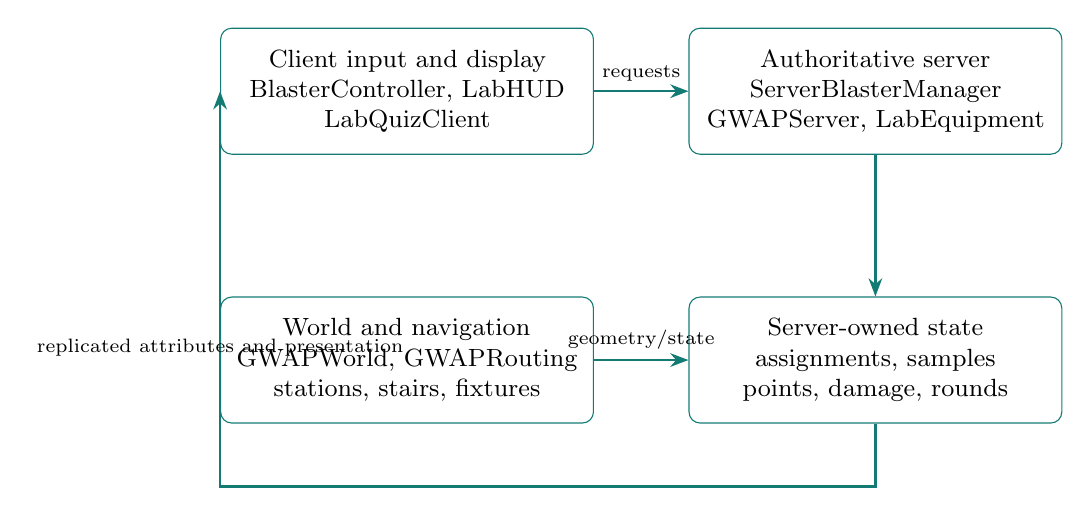
\begin{tikzpicture}[node distance=8mm,box/.style={draw=teal,rounded corners,align=center,text width=45mm,minimum height=16mm,font=\small},arr/.style={-{Stealth},thick,draw=teal}]
\node[box] (client) {Client input and display\\BlasterController, LabHUD\\LabQuizClient};
\node[box,right=12mm of client] (server) {Authoritative server\\ServerBlasterManager\\GWAPServer, LabEquipment};
\node[box,below=18mm of server] (state) {Server-owned state\\assignments, samples\\points, damage, rounds};
\node[box,below=18mm of client] (world) {World and navigation\\GWAPWorld, GWAPRouting\\stations, stairs, fixtures};
\draw[arr] (client.east) -- node[above,font=\scriptsize]{requests} (server.west);
\draw[arr] (server.south) -- (state.north);
\draw[arr] (world.east) -- node[above,font=\scriptsize]{geometry/state} (state.west);
\draw[arr] (state.south) -- ++(0,-8mm) -| node[pos=.7,below,font=\scriptsize]{replicated attributes and presentation} (client.west);
\end{tikzpicture}
\end{center}
Requests do not directly authorize rewards or damage. The server validates and commits gameplay state. The client displays that state and predicts visual aiming feedback. The world supplies geometry and station metadata; the current coordinate defect shows why those two must remain consistent.

\section{Observed origin mismatch: Incubator example}
\begin{center}
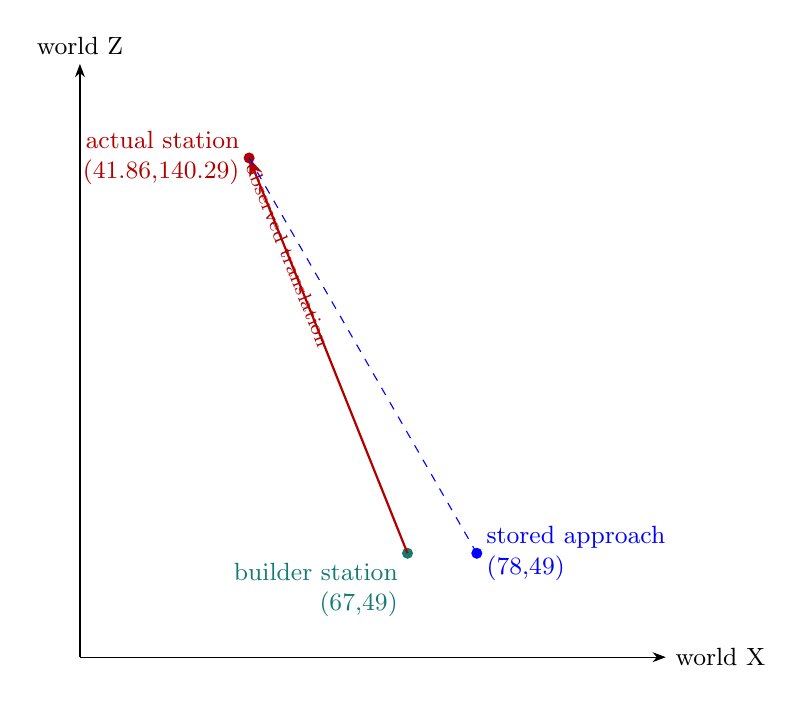
\begin{tikzpicture}[x=.08cm,y=.055cm,>=Stealth,font=\small]
\draw[->] (15,25) -- (108,25) node[right]{world X};
\draw[->] (15,25) -- (15,162) node[above]{world Z};
\fill[teal] (67,49) circle[radius=2pt] node[below left,align=right]{builder station\\(67,49)};
\fill[blue] (78,49) circle[radius=2pt] node[right,align=left]{stored approach\\(78,49)};
\fill[red!70!black] (41.857,140.286) circle[radius=2pt] node[left,align=right]{actual station\\(41.86,140.29)};
\draw[->,thick,red!70!black] (67,49) -- node[left,sloped,font=\scriptsize]{observed translation} (41.857,140.286);
\draw[dashed,blue] (78,49) -- (41.857,140.286);
\end{tikzpicture}
\end{center}
This plan view omits height for clarity. The station's actual Y is -21.75, while its builder Y is 1.5 and its stored approach Y is 3.25. Geometry translation does not automatically transform Vector3 attributes or literal coordinates in code. The dashed line illustrates the disagreement; it is not a proposed valid path.

\section{Proposed mission transition contract}
\begin{center}
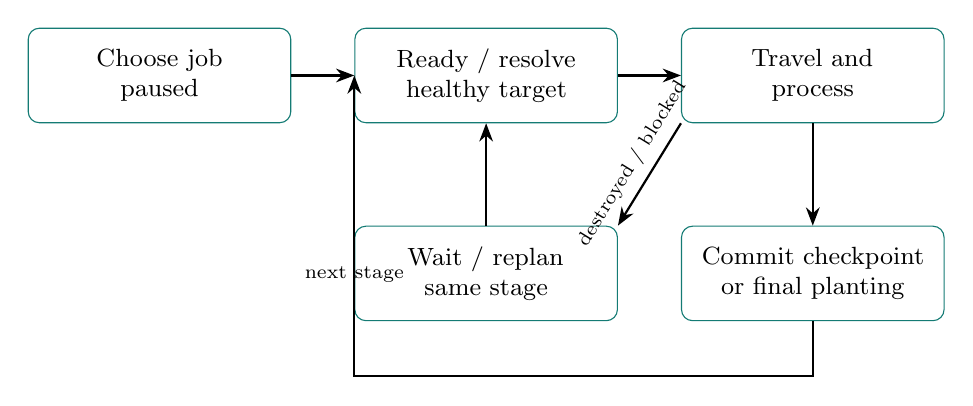
\begin{tikzpicture}[node distance=8mm,box/.style={draw=teal,rounded corners,align=center,text width=31mm,minimum height=12mm,font=\small},arr/.style={-{Stealth},thick}]
\node[box] (choose) {Choose job\\paused};
\node[box,right=8mm of choose] (resolve) {Ready / resolve\\healthy target};
\node[box,right=8mm of resolve] (travel) {Travel and\\process};
\node[box,below=13mm of travel] (commit) {Commit checkpoint\\or final planting};
\node[box,below=13mm of resolve] (wait) {Wait / replan\\same stage};
\draw[arr] (choose) -- (resolve);
\draw[arr] (resolve) -- (travel);
\draw[arr] (travel) -- (commit);
\draw[arr] (travel.south west) -- node[above,sloped,font=\scriptsize]{destroyed / blocked} (wait.north east);
\draw[arr] (wait) -- (resolve);
\draw[arr] (commit.south) -- ++(0,-7mm) -| node[pos=.7,below,font=\scriptsize]{next stage} (resolve.west);
\end{tikzpicture}
\end{center}
The current code implements destruction rerouting and pause behavior. General blocked-edge replanning remains proposed. Every asynchronous operation should carry the assignment/route revision so a stale operation cannot commit after regroup, termination, or a new target selection.

\chapter{Ten research scenarios: protocols and extension specifications}
All ten scenarios below are implemented as ordered gameplay routes and a randomized integer variant.\allowbreak{} The proposed data product and validation paragraphs are future design, not implemented science.\allowbreak{} Floor labels describe logical floors in the original building frame.\allowbreak{} The initial coordinate discrepancy was repaired in Revision 4; see its fresh verification results and remaining coverage limits.\allowbreak{}

\section{01.\allowbreak{} Germination viability}
\subsection{Implemented route and parameter}
Seed bank (B1) -> Incubator (L1) -> Plot 1 (roof)

Moisture, integer 35-80 percent

A seedling is collected, incubated, and planted.\allowbreak{} Moisture is a displayed assignment variant; it does not drive a germination probability model.\allowbreak{}

\subsection{Future scientific-purpose implementation}
Annotate germinated versus non-germinated seeds in authentic, protocol-controlled images.\allowbreak{} Store image ID, seed count, germination count, moisture condition, replicate, and observer decision.\allowbreak{}

Use known examples and repeated independent counts; compare agreement before interpreting treatment differences.\allowbreak{} Preserve the original image and sampling method.\allowbreak{}

\subsection{Engineering change and acceptance}
Try both endpoints of the moisture range; destroy the Incubator before arrival and during processing.\allowbreak{} Verify an equivalent is selected and the nominal two-checkpoint plus final reward is not duplicated.\allowbreak{}

Implementation touchpoints: GWAPScenarios defines title/\allowbreak{}purpose/\allowbreak{}route/\allowbreak{}range; GWAPWorld and GWAPRouting provide named capabilities and approaches; GWAPServer executes the stages and awards; LabHUD presents the assignment.\allowbreak{} A real data layer must add structured records independently of this route.\allowbreak{} Keep a stable scenario ID and protocol version so saved or exported observations do not change meaning when the list is reordered.\allowbreak{}

\section{02.\allowbreak{} Pathogen resistance}
\subsection{Implemented route and parameter}
Containment (L2) -> Bio-analyzer (L3) -> Plot 2 (roof)

Resistance batch, integer 1-9

The batch number distinguishes assignments.\allowbreak{} There is no infectious-agent simulation, measured resistance curve, or actual laboratory manipulation.\allowbreak{}

\subsection{Future scientific-purpose implementation}
Classify visible plant-damage severity in a vetted image dataset with blinded treatment labels.\allowbreak{} Store dataset item, scoring scale version, replicate, and confidence.\allowbreak{}

Use a researcher-defined severity rubric and reference examples.\allowbreak{} Separate plant damage from image artifacts; aggregate only comparable stages and cultivars.\allowbreak{}

\subsection{Engineering change and acceptance}
Destroy Containment and its same-floor backup, then confirm the other-floor replacement retains the same capability and stage.\allowbreak{} Check that resistance batch remains unchanged after rerouting.\allowbreak{}

Implementation touchpoints: GWAPScenarios defines title/\allowbreak{}purpose/\allowbreak{}route/\allowbreak{}range; GWAPWorld and GWAPRouting provide named capabilities and approaches; GWAPServer executes the stages and awards; LabHUD presents the assignment.\allowbreak{} A real data layer must add structured records independently of this route.\allowbreak{} Keep a stable scenario ID and protocol version so saved or exported observations do not change meaning when the list is reordered.\allowbreak{}

\section{03.\allowbreak{} Light spectrum optimization}
\subsection{Implemented route and parameter}
Seed bank (B1) -> Spectrograph (L2) -> Infrared scanner (L3) -> Plot 3 (roof)

Photoperiod, integer 8-18 hours

Three pre-plot stations create a longer route.\allowbreak{} The number of hours is descriptive, not elapsed game time or a measured spectrum.\allowbreak{}

\subsection{Future scientific-purpose implementation}
Mark leaf boundaries or estimate leaf area in calibrated images from controlled light treatments.\allowbreak{} Record calibration, illumination condition, image timestamp, and segmentation.\allowbreak{}

Require scale calibration and repeated annotation.\allowbreak{} Do not infer spectral response from the avatar visiting an instrument.\allowbreak{}

\subsection{Engineering change and acceptance}
Verify all four route stages and the nominal 105-point clean escort.\allowbreak{} Destroy the middle instrument after seed collection; the carrier must retain its seedling and resume without collecting a second one.\allowbreak{}

Implementation touchpoints: GWAPScenarios defines title/\allowbreak{}purpose/\allowbreak{}route/\allowbreak{}range; GWAPWorld and GWAPRouting provide named capabilities and approaches; GWAPServer executes the stages and awards; LabHUD presents the assignment.\allowbreak{} A real data layer must add structured records independently of this route.\allowbreak{} Keep a stable scenario ID and protocol version so saved or exported observations do not change meaning when the list is reordered.\allowbreak{}

\section{04.\allowbreak{} Soil bioremediation}
\subsection{Implemented route and parameter}
Chemical seedlings (B1) -> Root analyzer (L2) -> Plot 4 (roof)

Soil batch, integer 1-12

The workflow represents sample tracking.\allowbreak{} It does not calculate contaminant concentration, uptake, removal efficiency, or environmental safety.\allowbreak{}

\subsection{Future scientific-purpose implementation}
Trace roots in real scan images or match samples to verified metadata.\allowbreak{} Record source sample, imaging method, root mask, and uncertain regions.\allowbreak{}

Use expert review for ambiguous roots and preserve units/\allowbreak{}calibration.\allowbreak{} A gameplay completion cannot certify remediation success.\allowbreak{}

\subsection{Engineering change and acceptance}
Verify replacement Root analyzer selection, plot capacity, and no stage advancement while the target is destroyed.\allowbreak{} Confirm batch metadata remains associated with the assignment.\allowbreak{}

Implementation touchpoints: GWAPScenarios defines title/\allowbreak{}purpose/\allowbreak{}route/\allowbreak{}range; GWAPWorld and GWAPRouting provide named capabilities and approaches; GWAPServer executes the stages and awards; LabHUD presents the assignment.\allowbreak{} A real data layer must add structured records independently of this route.\allowbreak{} Keep a stable scenario ID and protocol version so saved or exported observations do not change meaning when the list is reordered.\allowbreak{}

\section{05.\allowbreak{} Hydroponic versus soil}
\subsection{Implemented route and parameter}
Split-root tray (L1) -> Centrifuge (L3) -> Root analyzer (L2) -> Plot 5 (roof)

Nutrient batch, integer 1-8

The route deliberately goes up and then down before the roof.\allowbreak{} No paired root-growth measurements currently exist.\allowbreak{}

\subsection{Future scientific-purpose implementation}
Compare paired, anonymized root images from controlled growth conditions.\allowbreak{} Store pair ID, condition metadata held separately, root-length annotation, and replicate.\allowbreak{}

Randomize presentation order and require comparable imaging scales.\allowbreak{} Analyze pairs rather than treating unrelated plants as matched samples.\allowbreak{}

\subsection{Engineering change and acceptance}
Exercise both ascent and descent, a destroyed Centrifuge, and a destroyed Root analyzer.\allowbreak{} Check that the route order is preserved and the two instruments are not treated as interchangeable.\allowbreak{}

Implementation touchpoints: GWAPScenarios defines title/\allowbreak{}purpose/\allowbreak{}route/\allowbreak{}range; GWAPWorld and GWAPRouting provide named capabilities and approaches; GWAPServer executes the stages and awards; LabHUD presents the assignment.\allowbreak{} A real data layer must add structured records independently of this route.\allowbreak{} Keep a stable scenario ID and protocol version so saved or exported observations do not change meaning when the list is reordered.\allowbreak{}

\section{06.\allowbreak{} UV adaptation}
\subsection{Implemented route and parameter}
UV chamber (L2) -> Vitality scanner (L1) -> Plot 6 (roof)

Exposure, integer 5-20 seconds

The assignment text describes exposure; processing is still the common four-second gameplay action and does not implement the chosen duration.\allowbreak{}

\subsection{Future scientific-purpose implementation}
Annotate visible stress features in a curated before/\allowbreak{}after plant image pair.\allowbreak{} Record acquisition conditions, treatment metadata, severity features, and uncertainty.\allowbreak{}

Use researcher-approved image data and a fixed rubric.\allowbreak{} This game is not an instruction for operating UV equipment.\allowbreak{}

\subsection{Engineering change and acceptance}
Check descending travel after the UV stage, stable variant display, and shared use of Vitality scanner capability with scenarios 10 and 6 without crossing assignment ownership.\allowbreak{}

Implementation touchpoints: GWAPScenarios defines title/\allowbreak{}purpose/\allowbreak{}route/\allowbreak{}range; GWAPWorld and GWAPRouting provide named capabilities and approaches; GWAPServer executes the stages and awards; LabHUD presents the assignment.\allowbreak{} A real data layer must add structured records independently of this route.\allowbreak{} Keep a stable scenario ID and protocol version so saved or exported observations do not change meaning when the list is reordered.\allowbreak{}

\section{07.\allowbreak{} Gravitropism assay}
\subsection{Implemented route and parameter}
Clinostat (B1) -> Orientation scanner (L1) -> Plot 7 (roof)

Tray tilt, integer 10-80 degrees

The scenario names an orientation experiment but does not currently simulate root curvature from gravity or time.\allowbreak{}

\subsection{Future scientific-purpose implementation}
Mark root tips and growth angles in time-lapse frames with a known reference axis.\allowbreak{} Store frame time, axis calibration, landmarks, and annotation quality.\allowbreak{}

Require consistent angle conventions and reject occluded frames.\allowbreak{} Separate tray orientation from measured root direction.\allowbreak{}

\subsection{Engineering change and acceptance}
Verify Clinostat backups, floor-label conversion for basement, and a clear initial rendezvous.\allowbreak{} Test the zero-length initial-path case that previously required an explicit bypass.\allowbreak{}

Implementation touchpoints: GWAPScenarios defines title/\allowbreak{}purpose/\allowbreak{}route/\allowbreak{}range; GWAPWorld and GWAPRouting provide named capabilities and approaches; GWAPServer executes the stages and awards; LabHUD presents the assignment.\allowbreak{} A real data layer must add structured records independently of this route.\allowbreak{} Keep a stable scenario ID and protocol version so saved or exported observations do not change meaning when the list is reordered.\allowbreak{}

\section{08.\allowbreak{} Drought resistance}
\subsection{Implemented route and parameter}
Climate chamber (L3) -> Porometer (L2) -> Plot 8 (roof)

Humidity, integer 20-45 percent

The mission says simulated stomatal response, but it does not compute conductance or water potential.\allowbreak{} Humidity is assignment metadata.\allowbreak{}

\subsection{Future scientific-purpose implementation}
Annotate stomatal aperture from suitable microscopy images or organize verified instrument observations.\allowbreak{} Store image/\allowbreak{}instrument record ID, scale, treatment, aperture annotation, and replicate.\allowbreak{}

Require a defined measurement method and expert validation.\allowbreak{} Do not combine incompatible instruments or units under one generic score.\allowbreak{}

\subsection{Engineering change and acceptance}
Destroy the Porometer while the carrier is processing; verify that processing restarts at an equivalent rather than completing on the destroyed station.\allowbreak{}

Implementation touchpoints: GWAPScenarios defines title/\allowbreak{}purpose/\allowbreak{}route/\allowbreak{}range; GWAPWorld and GWAPRouting provide named capabilities and approaches; GWAPServer executes the stages and awards; LabHUD presents the assignment.\allowbreak{} A real data layer must add structured records independently of this route.\allowbreak{} Keep a stable scenario ID and protocol version so saved or exported observations do not change meaning when the list is reordered.\allowbreak{}

\section{09.\allowbreak{} Microbiome symbiosis}
\subsection{Implemented route and parameter}
Wet lab (B1) -> Symbiosis incubator (L2) -> Plot 9 (roof)

Inoculum batch, integer 1-8

The batch labels a transport protocol.\allowbreak{} No microbial growth model, sequencing data, or biological assay is present.\allowbreak{}

\subsection{Future scientific-purpose implementation}
Label root colonization regions in an approved microscopy dataset.\allowbreak{} Store image ID, region mask, labeling taxonomy, batch, and replicate.\allowbreak{}

Use blinded examples, inter-annotator agreement, and expert adjudication.\allowbreak{} Treat uncertain regions as uncertain rather than forcing a positive classification.\allowbreak{}

\subsection{Engineering change and acceptance}
Verify the carrier spawns near the selected role, explains the assignment, waits for Ready, and retains the inoculum batch through same-floor and other-floor reroutes.\allowbreak{}

Implementation touchpoints: GWAPScenarios defines title/\allowbreak{}purpose/\allowbreak{}route/\allowbreak{}range; GWAPWorld and GWAPRouting provide named capabilities and approaches; GWAPServer executes the stages and awards; LabHUD presents the assignment.\allowbreak{} A real data layer must add structured records independently of this route.\allowbreak{} Keep a stable scenario ID and protocol version so saved or exported observations do not change meaning when the list is reordered.\allowbreak{}

\section{10.\allowbreak{} Cold-hardiness screening}
\subsection{Implemented route and parameter}
Cryo-freezer (B1) -> Vitality scanner (L1) -> Plot 10 (roof)

Recovery temperature, integer 5-20 C

The workflow models recovery transport.\allowbreak{} It does not simulate freezing injury or measure actual survival.\allowbreak{}

\subsection{Future scientific-purpose implementation}
Score recovery features in a time series with known treatment conditions.\allowbreak{} Store plant ID, time since recovery, visible features, viability rubric, and observer confidence.\allowbreak{}

Require consistent follow-up timing and a definition of survival.\allowbreak{} Separate missing observations from dead plants.\allowbreak{}

\subsection{Engineering change and acceptance}
Check cryo-freezer explosion handling, a full Plot 10 falling back to another healthy greenhouse plot, and no reward if the assigned carrier is intercepted before final planting.\allowbreak{}

Implementation touchpoints: GWAPScenarios defines title/\allowbreak{}purpose/\allowbreak{}route/\allowbreak{}range; GWAPWorld and GWAPRouting provide named capabilities and approaches; GWAPServer executes the stages and awards; LabHUD presents the assignment.\allowbreak{} A real data layer must add structured records independently of this route.\allowbreak{} Keep a stable scenario ID and protocol version so saved or exported observations do not change meaning when the list is reordered.\allowbreak{}


\chapter{Defect register, change accounting, and lessons}
\section{How many bugs were generated?}
The evidence supports a bounded register of 24 historical defect families (H01-H24), two newly observed source/\allowbreak{}scene discrepancies (C01-C02), seven baseline audit risks (R01-R07), with final status in the Revision 4 chapter, and two tool/\allowbreak{}test artifacts (T01-T02).\allowbreak{} These categories are not added together as a lifetime bug total.\allowbreak{} A family groups recurring reports of the same symptom; one family may have had several causes or fixes.\allowbreak{} No complete issue tracker, commit history, or causal record establishes the total number of bugs introduced by an AI model.\allowbreak{}

At least two episodes have explicit evidence of an AI change or implementation error: H13 is the owner-requested rollback/\allowbreak{}restoration after an aiming change, and H24 is the zero-length route-prefix defect encountered during implementation testing.\allowbreak{} Other families are associated with the evolving AI-built game, but the record does not isolate whether each was newly introduced, pre-existing, or caused by an intervening model/\allowbreak{}asset change.\allowbreak{} Reporting all 24 as definitely generated by one model would be unsupported.\allowbreak{} The two current discrepancies are observed now; their author and exact introduction time are unknown.\allowbreak{}

Five major requirement reversals are recorded separately: large monitor panels were later removed; quizzes were added, removed, and then reintroduced in simpler form; the extra GWAP arsenal was added and then rejected; a broad 60-percent failure policy was replaced by a small workload; and static/\allowbreak{}identical NPC presentations were replaced by differentiated moving workers.\allowbreak{} New research-equipment destructibility and equivalent-station rerouting are feature extensions as well as corrections to the desired experience.\allowbreak{} They do not each count automatically as a new software bug.\allowbreak{}

\section{Historical defect families}
\subsection{H01: Role kiosk inaccessible or inert}
Evidence: Earlier shared chat: user could not select a role or activate the kiosk.\allowbreak{}

Repair history: Interaction layout and trigger behavior were repeatedly revised; temporary touch selection was later removed.\allowbreak{}

Code and regression target: LabRoles and kiosk geometry; verify E/\allowbreak{}click selection and no accidental role change.\allowbreak{}

Status: Reported fixed historically; not replayed in this edition.\allowbreak{}

\subsection{H02: Role outfit missing or insufficiently distinct}
Evidence: Earlier shared chat repeatedly requested visible clothing after role selection.\allowbreak{}

Repair history: Role appearance application and respawn behavior were revised.\allowbreak{}

Code and regression target: LabRoles; test both roles before and after respawn.\allowbreak{}

Status: Reported fixed historically; appearance is built, full rig coverage unverified.\allowbreak{}

\subsection{H03: Equipment E/\allowbreak{}F actions appeared inert}
Evidence: Earlier user reports said nothing happened near equipment or when pressing controls.\allowbreak{}

Repair history: Physical prompts/\allowbreak{}buttons and runtime/\allowbreak{}fallback installation were revised.\allowbreak{}

Code and regression target: LabEquipment bind/\allowbreak{}makeControls; distinguish old F behavior from current E/\allowbreak{}R policy.\allowbreak{}

Status: Reported fixed historically; syntax checks alone were insufficient evidence.\allowbreak{}

\subsection{H04: Plant could be taken but not dropped}
Evidence: Earlier user explicitly reported pickup without a usable drop interaction.\allowbreak{}

Repair history: Working-cabinet drop logic, free-slot guidance, and human override of reservations were improved.\allowbreak{}

Code and regression target: LabEquipment takePlantFromChamber/\allowbreak{}storePlantInChamber.\allowbreak{}

Status: Reported fixed historically; retest full/\allowbreak{}wrong/\allowbreak{}removed destinations.\allowbreak{}

\subsection{H05: Equipment or fixtures intersected walls, doors, or windows}
Evidence: Multiple earlier screenshots and requests identified misplaced cabinets, health kits, weapons, and pipes.\allowbreak{}

Repair history: Placement clearance and wall alignment were revised; pipes moved upward.\allowbreak{}

Code and regression target: Generator placement and saved geometry.\allowbreak{}

Status: Historical clearance measurements exist; current translated geometry needs a fresh spatial audit.\allowbreak{}

\subsection{H06: Equipment could be repaired through a wall}
Evidence: Earlier user explicitly identified repair across a wall.\allowbreak{}

Repair history: Closer interaction range and server line-of-sight validation were added to legacy interactions.\allowbreak{}

Code and regression target: LabEquipment canInteract.\allowbreak{}

Status: Built in legacy path; separate research prompts have risk R01.\allowbreak{}

\subsection{H07: Repair route crossed walls or ignored stairs}
Evidence: Earlier user reported a straight red path through geometry.\allowbreak{}

Repair history: Pathfinding and explicit stair-aware routing replaced a straight fallback.\allowbreak{}

Code and regression target: LabEquipment createRepairPath; later GWAP routePoints is a separate implementation.\allowbreak{}

Status: Historically reported fixed; C01 invalidates assumptions for moved geometry.\allowbreak{}

\subsection{H08: Overlapping information obscured play}
Evidence: Repeated shared-chat and current-thread screenshots show large or duplicate panels.\allowbreak{}

Repair history: Distant labels, duplicate HUDs, and notification feeds were reduced; latest HUD groups mission/\allowbreak{}status.\allowbreak{}

Code and regression target: LabHUD, LabEquipment display policy, BlasterController, LabQuizClient.\allowbreak{}

Status: One small-phone layout measured; all modals/\allowbreak{}devices not exhaustive.\allowbreak{}

\subsection{H09: Uneven lighting and black floor bands}
Evidence: Earlier handoff requested lighting repair.\allowbreak{}

Repair history: The handoff records the defect but does not independently prove the exact repair.\allowbreak{}

Code and regression target: Generator Lighting and room light placement.\allowbreak{}

Status: Historical report; current visual closure not established by this audit.\allowbreak{}

\subsection{H10: Touch firing failed or used unsuitable input}
Evidence: Shared chat requested cross-platform shooting because mobile controls failed.\allowbreak{}

Repair history: Separated controller, casting module, and server manager; touch camera and action controls introduced.\allowbreak{}

Code and regression target: BlasterController, Blaster, ServerBlasterManager.\allowbreak{}

Status: Historical device checks reported; preserve input separation.\allowbreak{}

\subsection{H11: Reticle and muzzle impact disagreed}
Evidence: Shared chat reported firing toward the avatar or not correctly hitting a wall.\allowbreak{}

Repair history: Camera target and muzzle obstruction handling were revised.\allowbreak{}

Code and regression target: Blaster ray helpers and controller reticle.\allowbreak{}

Status: Historical desktop/\allowbreak{}mobile impact checks reported.\allowbreak{}

\subsection{H12: Android vertical aim offset}
Evidence: Aiming at the tree base produced a hit near the branches.\allowbreak{}

Repair history: Mobile ray changed to Camera.\allowbreak{}CFrame.\allowbreak{}LookVector after a reported 1.\allowbreak{}35-degree safe-area mismatch.\allowbreak{}

Code and regression target: BlasterController mobile aim ray.\allowbreak{}

Status: Historical lower-trunk hit and client/\allowbreak{}server direction agreement reported.\allowbreak{}

\subsection{H13: Mouse pitch/\allowbreak{}yaw and arm tracking regressed}
Evidence: User requested restoration after unrelated trigger/\allowbreak{}aim experiments.\allowbreak{}

Repair history: Mouse-priority detection and shoulder/\allowbreak{}arm target tracking restored, including newer joints.\allowbreak{}

Code and regression target: BlasterController input mode and arm pose.\allowbreak{}

Status: Explicit AI-change-associated regression; historically restored.\allowbreak{}

\subsection{H14: FIRE/\allowbreak{}AIM/\allowbreak{}JUMP controls overlapped}
Evidence: Shared chat and screenshots identified overlapping mobile actions.\allowbreak{}

Repair history: Controls repositioned relative to jump with separate spacing.\allowbreak{}

Code and regression target: BlasterController touch layout.\allowbreak{}

Status: Historical Galaxy A06 check; regression coverage required after HUD changes.\allowbreak{}

\subsection{H15: HUD existed without its reticle}
Evidence: Shared chat reports incomplete BlasterHUD initialization.\allowbreak{}

Repair history: HUD integrity checks rebuild missing reticle children.\allowbreak{}

Code and regression target: BlasterController \_\allowbreak{}ensureHUD.\allowbreak{}

Status: Reported fixed historically; test equip/\allowbreak{}unequip and device changes.\allowbreak{}

\subsection{H16: Maintenance vent landed player partly in floor}
Evidence: User reported becoming embedded at basement destination.\allowbreak{}

Repair history: Vent landing and both basement stair routes were corrected.\allowbreak{}

Code and regression target: LabEquipment basement handler and generator geometry.\allowbreak{}

Status: Historical vent landing test reported.\allowbreak{}

\subsection{H17: Workers passed through geometry or players}
Evidence: Shared chat requested room-aware movement and avoidance.\allowbreak{}

Repair history: Original worker motion gained room/\allowbreak{}obstacle checks and appearance updates.\allowbreak{}

Code and regression target: LabEquipment botMotionChecks/\allowbreak{}walkBotSegment/\allowbreak{}moveBotTo.\allowbreak{}

Status: Historical implementation; not proof of arbitrary carrier obstacle avoidance.\allowbreak{}

\subsection{H18: Assigned carrier was not nearby or visible}
Evidence: Current-thread user could not find the mission NPC after role selection.\allowbreak{}

Repair history: Per-player companion allocation and safe nearby placement introduced.\allowbreak{}

Code and regression target: GWAPServer companion/\allowbreak{}startMission; GWAPNPC nearPlayer.\allowbreak{}

Status: Historical approximately eight-stud placement test.\allowbreak{}

\subsection{H19: Carrier clones repeated names/\allowbreak{}appearance and female silhouette was wrong}
Evidence: Current-thread screenshots show repeated Maria models and unsuitable hair.\allowbreak{}

Repair history: Different non-seated templates, alternating gender preference, and hair adjustments.\allowbreak{}

Code and regression target: GWAPServer makeBot; GWAPNPC appearance.\allowbreak{}

Status: Historical appearance check; animation/\allowbreak{}identity remain template-dependent.\allowbreak{}

\subsection{H20: Carriers queued together in the hallway}
Evidence: Current-thread screenshot and request rejected a hallway line of bots.\allowbreak{}

Repair history: Unused carriers moved to a ServerStorage pool and allocated individually.\allowbreak{}

Code and regression target: GWAPServer available/\allowbreak{}companions/\allowbreak{}pool.\allowbreak{}

Status: Historical one visible, four pooled observation.\allowbreak{}

\subsection{H21: Carrier glided unnaturally and too slowly}
Evidence: Current-thread user asked for natural movement matching player speed.\allowbreak{}

Repair history: Distance-driven limb gait and smoothed owner WalkSpeed matching added.\allowbreak{}

Code and regression target: GWAPNPC animate; GWAPServer go.\allowbreak{}

Status: Historical speed-20 movement and approximately 24-degree leg swing measured.\allowbreak{}

\subsection{H22: Weapon trembled while idle and walking}
Evidence: Repeated current-thread reports persisted after an earlier partial fix.\allowbreak{}

Repair history: Single pre-camera rotation, no artificial Grip bob, and armed animation stabilization.\allowbreak{}

Code and regression target: BlasterController pre-camera, render, and PreSimulation paths.\allowbreak{}

Status: Historical zero Grip motion idle/\allowbreak{}walking; firing recoil retained.\allowbreak{}

\subsection{H23: Wall explosion left fixtures floating or usable}
Evidence: Current-thread user requested disappearance of objects attached to the removed wall section.\allowbreak{}

Repair history: Recent-blast wall removal detection and fixture quarantine introduced.\allowbreak{}

Code and regression target: GWAPWallDamage.\allowbreak{}

Status: Historical four fixture categories removed; outside health station preserved.\allowbreak{}

\subsection{H24: Zero-length rendezvous path prevented progress}
Evidence: Development test encountered a start point already at its corridor entry.\allowbreak{}

Repair history: Zero-distance prefix bypass and checked short direct path added.\allowbreak{}

Code and regression target: GWAPServer go initial rendezvous.\allowbreak{}

Status: Implementation-level defect found during testing; historical retest passed.\allowbreak{}

\section{Baseline discrepancies, risks, and tool artifacts}
These entries preserve the initial audit.\allowbreak{} Revision 4 repairs C01/\allowbreak{}C02, adds role/\allowbreak{}LOS validation for R01, collision stopping for R02, correct eligibility for R03, and filtering for R07.\allowbreak{} R04 restoration policy, R05 shared-mission semantics, R06 load certification and the limits stated in the Revision 4 chapter remain open.\allowbreak{}

\subsection{C01: Observed now: moved geometry, stale route coordinates}
Evidence: Station positions and roof share a translation while Approach attributes and routePoints constants retain the old origin.\allowbreak{}

Next action: Introduce a coherent local coordinate frame and approach attachments; validate every route in a copied place.\allowbreak{} No fix installed here.\allowbreak{}

\subsection{C02: Observed now: incorrect world module bundled in installer}
Evidence: Root GWAPWorld.\allowbreak{}lua contains older mission-server code, and InstallGWAP.\allowbreak{}lua installs that incorrect content as the world module.\allowbreak{} The active module is different.\allowbreak{}

Next action: Do not run the captured installer unchanged.\allowbreak{} Replace its world-module input from the verified active source, reconcile generator versions, regenerate and compare installed hashes in a copied place.\allowbreak{}

\subsection{R01: Research prompt validation is narrower than legacy validation}
Evidence: ResearchRepair checks life, distance, and Exploded but does not enforce Technician role or perform its own server ray visibility check.\allowbreak{}

Next action: Apply an explicit role/\allowbreak{}range/\allowbreak{}visibility/\allowbreak{}state policy and validate hold completion server-side where required.\allowbreak{} Test wrong role and an intervening wall.\allowbreak{}

\subsection{R02: Main carrier route assumes clear surveyed geometry}
Evidence: The main kinematic route moves along points and stops near players; it does not sweep every segment for arbitrary new obstacles.\allowbreak{}

Next action: Add edge validation, blocked-route state, and bounded replanning.\allowbreak{} Preserve one movement authority.\allowbreak{}

\subsection{R03: Solo percentage counts pooled models}
Evidence: Arming includes available carriers outside Workspace, while shooting excludes them.\allowbreak{}

Next action: Define an eligible active population; recompute selection on lifecycle changes and display both selected and active threat counts.\allowbreak{}

\subsection{R04: Wall-fixture restoration is not defined}
Evidence: Removed fixtures remain in ServerStorage; repairing attributes does not rebuild walls or reparent fixtures.\allowbreak{}

Next action: Define persistent versus per-round destruction, then implement explicit restoration or deliberate permanent removal for the session.\allowbreak{}

\subsection{R05: Multiplayer balance and shared objective semantics are unverified}
Evidence: Assignments are per player; no complete multi-client regression was recorded.\allowbreak{}

Next action: Test two roles and multiple carriers concurrently; commission a shared-convoy design separately if desired.\allowbreak{}

\subsection{R06: Scale is configured, not performance-certified}
Evidence: MaxPlayers is 60 and the scene is large; no current load profile was captured.\allowbreak{}

Next action: Measure client/\allowbreak{}server frame time, memory, replication, and NPC workloads before making capacity claims.\allowbreak{}

\subsection{R07: Lounge notes are displayed without explicit filtering}
Evidence: LoungeSystems onChat stores the raw /\allowbreak{}note message and refreshWall writes it to a shared display; no text-filtering call appears in that source.\allowbreak{}

Next action: Filter submitted text on the server using the appropriate Roblox text-filtering result for a shared display, handle filtering failure without displaying raw text, and add length/\allowbreak{}rate limits.\allowbreak{} Test with multiple viewers.\allowbreak{}

\subsection{T01: Tool artifact: truncated source backup}
Evidence: A previous LabEquipment backup was cut near 100 KB and renamed .\allowbreak{}partial.\allowbreak{}lua.\allowbreak{}

Next action: Never install a partial capture.\allowbreak{} This edition verifies every reconstructed Studio source byte length.\allowbreak{}

\subsection{T02: Test artifact: duplicate controller binding}
Evidence: A prior client test required/\allowbreak{}bound a controller again and produced duplicate render-step warnings.\allowbreak{}

Next action: Use existing bootstrap/\allowbreak{}controller instances for probes and fresh Play sessions; do not classify the test harness warning as a confirmed production defect.\allowbreak{}

\section{Rules that prevent repetition}
Freeze an accepted input/\allowbreak{}camera baseline before unrelated features.\allowbreak{} Measure a symptom before rewriting its subsystem.\allowbreak{} Use live source and hashes to resolve conflicts.\allowbreak{} Keep one owner for camera, root, arm, and gun transforms.\allowbreak{} Revalidate after every yielding interaction.\allowbreak{} Treat geometry and navigation metadata as one versioned unit.\allowbreak{} Check actual screen rectangles and server state, not only appearance.\allowbreak{} Separate a passing syntax check from a passing player workflow.\allowbreak{} Never report a tool artifact or an old test as proof of current gameplay correctness.\allowbreak{}


\chapter{Verification ledger and future acceptance suite}
\section{P01: Role selection and nearby companion}
Evidence period: Prior GWAP turn

Observed/\allowbreak{}reported result: Approximately eight studs from player; one visible carrier and four pooled.\allowbreak{}

Limit: Historical observation, not rerun for current geometry.\allowbreak{}

\section{P02: Wait and Regroup}
Evidence period: Prior GWAP turn

Observed/\allowbreak{}reported result: Wait movement zero; regroup returned within roughly eight studs.\allowbreak{}

Limit: No stress test of every blocked spawn candidate.\allowbreak{}

\section{P03: Original rifle and equipment destruction}
Evidence period: Prior GWAP turn

Observed/\allowbreak{}reported result: Lab Rifle destroyed a research machine; nearby explosion destroyed another; R repair restored it.\allowbreak{}

Limit: Does not certify wall-fixture restoration or every blast chain.\allowbreak{}

\section{P04: Equivalent rerouting}
Evidence period: Prior GWAP turn

Observed/\allowbreak{}reported result: Incubator -> same-floor Backup 1 -> other-floor Backup 2; assignment stayed RUNNING.\allowbreak{}

Limit: Earlier coordinate frame; current C01 requires rerun.\allowbreak{}

\section{P05: Carrier gait and speed}
Evidence period: Prior GWAP turn

Observed/\allowbreak{}reported result: WalkSpeed 20; roughly 28.\allowbreak{}7 studs of travel during sampled interval; leg swing about 24 degrees.\allowbreak{}

Limit: Kinematic gait, not Humanoid physics certification.\allowbreak{}

\section{P06: Wall-fixture cleanup}
Evidence period: Prior GWAP turn

Observed/\allowbreak{}reported result: Four fixture types within a temporary wall section removed; outside health station preserved.\allowbreak{}

Limit: Controlled isolated test, not whole-floor blast profiling.\allowbreak{}

\section{P07: Small mobile layout}
Evidence period: Prior GWAP turn

Observed/\allowbreak{}reported result: 705x338 viewport; panel bottom y=179, joystick top y=187.\allowbreak{}

Limit: Eight-pixel gap in this configuration only.\allowbreak{}

\section{P08: Idle weapon stabilization}
Evidence period: Prior GWAP turn

Observed/\allowbreak{}reported result: 90 frames with zero Grip motion and zero shoulder-animation translation.\allowbreak{}

Limit: One tested original rifle/\allowbreak{}rig configuration.\allowbreak{}

\section{P09: Walking stabilization}
Evidence period: Prior GWAP turn

Observed/\allowbreak{}reported result: Approximately 19 studs of walking with zero Grip motion.\allowbreak{}

Limit: Intentional recoil while firing was not removed.\allowbreak{}

\section{P10: Interception score}
Evidence period: Prior GWAP turn

Observed/\allowbreak{}reported result: Assigned carrier awarded 50 once; repeat damage did not add points.\allowbreak{}

Limit: Multi-client race conditions not exhaustively tested.\allowbreak{}

\section{P11: Solo score loss}
Evidence period: Prior GWAP turn

Observed/\allowbreak{}reported result: 100 points became 99 on a successful NPC hit.\allowbreak{}

Limit: Low-score fractional policy also inspected in code; no long statistical run.\allowbreak{}

\section{P12: Rooftop mission completion}
Evidence period: Earlier GWAP turn

Observed/\allowbreak{}reported result: Seed source -> instrument -> roof completed and one plant appeared.\allowbreak{}

Limit: Test used helper following; friendly fire disqualified final escort reward, so clean full reward was not proven.\allowbreak{}

\section{P13: Player shooting validation}
Evidence period: Shared chat

Observed/\allowbreak{}reported result: Reported 10 damage, wall blocking, and rejection of distant forged camera origin.\allowbreak{}

Limit: Historical report; not a new penetration/\allowbreak{}security audit.\allowbreak{}

\section{P14: ADS and device controls}
Evidence period: Shared chat

Observed/\allowbreak{}reported result: Reported FOV 70->55 and sensitivity 1->0.\allowbreak{}62, restored on exit; phone/\allowbreak{}tablet controls checked.\allowbreak{}

Limit: Some later control changes superseded these exact UI versions.\allowbreak{}

\section{P15: Basement and quiz/\allowbreak{}window interactions}
Evidence period: Shared chat

Observed/\allowbreak{}reported result: Vent landing, pickup quiz, and breakable window passed reported checks.\allowbreak{}

Limit: No new Play session in this edition.\allowbreak{}

\section{D01: Live source completeness}
Evidence period: This edition

Observed/\allowbreak{}reported result: 29 source containers captured; every UTF-8 byte length matched Studio inventory.\allowbreak{}

Limit: Static capture only; active count 20, archive 8, disabled generator 1.\allowbreak{}

\section{D02: Scene/\allowbreak{}source audit}
Evidence period: This edition

Observed/\allowbreak{}reported result: 67 research station records; place version 70; C01 and C02 identified.\allowbreak{}

Limit: No claim that current routing is playable.\allowbreak{}

\section{Proposed new regression sequence}
\subsection{Baseline}
Open a copied saved place, identify the place/\allowbreak{}version, compare active-source hashes, and ensure there is only one bootstrap/\allowbreak{}controller authority.\allowbreak{}

\subsection{Coordinate frame}
Translate and rotate a test laboratory with its navigation origin; verify every station approach stays in its intended corridor and each stair edge is clear.\allowbreak{} Include the current displaced scene as a regression fixture.\allowbreak{}

\subsection{Transactions}
Two clients compete for the same plant and destination slot.\allowbreak{} Exactly one transfer commits; the other gets a clear reason.\allowbreak{} Repeat with a quiz outstanding, a full cabinet, and a destroyed destination.\allowbreak{}

\subsection{Carrier lifecycle}
Choose, Ready, Wait, Status, Regroup, respawn, disconnect, change role, and end the round during travel and processing.\allowbreak{} No duplicate carrier, seedling, or reward remains.\allowbreak{}

\subsection{Destruction}
Bullet-hit research station, chain blast, wall-section removal, outside-fixture preservation, repair, all-equivalents unavailable, and round reset after quarantine.\allowbreak{}

\subsection{Input preservation}
Desktop mouse target at all screen edges; mobile forward ray; right-swipe camera with left movement; ADS on/\allowbreak{}off; equip/\allowbreak{}unequip; idle/\allowbreak{}walk gun stability; UI click does not fire.\allowbreak{}

\subsection{Responsive layout}
Small phone portrait and landscape, tablet, desktop, chat open, quiz open, inventory open.\allowbreak{} Record rectangle intersections for mission, joystick, jump, fire, aim, and prompts.\allowbreak{}

\subsection{Scoring}
Clean 90/\allowbreak{}105-point escort as applicable, one 50-point interception, friendly-fire disqualification, low-score fractional loss, reset debt, and multiplayer solo-fire exclusion.\allowbreak{}

\subsection{Performance}
Profile crowded rooms and multi-client play; report hardware, viewport, scene population, average/\allowbreak{}p95 frame time, server heartbeat cost, and replication load.\allowbreak{} Do not extrapolate a one-client test to 60 players.\allowbreak{}

These are proposed tests.\allowbreak{} They were not executed while producing this document.\allowbreak{} The verification report for this edition concerns source capture, document compilation, page rendering, and manifest completeness.\allowbreak{}


\chapter{Subsystem-by-subsystem future update playbook}
\section{LabKinds: Equipment catalog}
Authoritative source: S05 /\allowbreak{} ReplicatedStorage.\allowbreak{}LabKinds

See complete listing on page \pageref{src:S05}.

\subsection{Proposed implementation}
Add one Kind with inputs, outputs, wait duration, and display text.\allowbreak{} Keep simulation values explicit.\allowbreak{}

\subsection{Dependencies to preserve}
LabEquipment consumption and treatment paths; generator Kind attributes.\allowbreak{}

\subsection{Acceptance cases}
Unknown Kind, missing input, invalid output, full destination, and a complete valid cycle.\allowbreak{}

\section{LabEquipment: Equipment engine}
Authoritative source: S11 /\allowbreak{} ServerScriptService.\allowbreak{}LabEquipment

See complete listing on page \pageref{src:S11}.

\subsection{Proposed implementation}
Extract inventory transactions before touching hazards or NPC motion.\allowbreak{} Preserve reservations and post-yield validation.\allowbreak{}

\subsection{Dependencies to preserve}
LabRoles assignments, LabQuizClient, tagged geometry, server hit bridge.\allowbreak{}

\subsection{Acceptance cases}
Concurrent pickup/\allowbreak{}drop, repair during failure tick, dead player, destroyed target, canceled quiz.\allowbreak{}

\section{LabRoles: Roles and outfits}
Authoritative source: S12 /\allowbreak{} ServerScriptService.\allowbreak{}LabRoles

See complete listing on page \pageref{src:S12}.

\subsection{Proposed implementation}
Keep exactly two roles unless commissioned otherwise; centralize role-to-outfit and permission mapping.\allowbreak{}

\subsection{Dependencies to preserve}
GWAPServer LabRole observer and original equipment role checks.\allowbreak{}

\subsection{Acceptance cases}
Both kiosks, respawn, role change during mission, and accessory/\allowbreak{}rig variations.\allowbreak{}

\section{LabRound: Round lifecycle}
Authoritative source: S13 /\allowbreak{} ServerScriptService.\allowbreak{}LabRound

See complete listing on page \pageref{src:S13}.

\subsection{Proposed implementation}
Make reset ordering explicit with one round transition contract and subsystem callbacks.\allowbreak{}

\subsection{Dependencies to preserve}
Points, fractional debt, carrier termination, research repair, plot clearing.\allowbreak{}

\subsection{Acceptance cases}
Join during break, end during processing, disconnected winner, and reset after destruction.\allowbreak{}

\section{LabTechnicians: Legacy worker service}
Authoritative source: S14 /\allowbreak{} ServerScriptService.\allowbreak{}LabTechnicians

See complete listing on page \pageref{src:S14}.

\subsection{Proposed implementation}
Check which templates actually have Humanoids before extending its path loop.\allowbreak{} Avoid competing with LabEquipment worker motion.\allowbreak{}

\subsection{Dependencies to preserve}
LabWorkerBot tags and template structure.\allowbreak{}

\subsection{Acceptance cases}
No double movement, no idle thread leak, valid target assignment, and bounded retry.\allowbreak{}

\section{LabElevators: Elevator compatibility script}
Authoritative source: S10 /\allowbreak{} ServerScriptService.\allowbreak{}LabElevators

See complete listing on page \pageref{src:S10}.

\subsection{Proposed implementation}
Treat as dormant unless real tagged elevator geometry exists.\allowbreak{} Do not claim elevator transport from script presence alone.\allowbreak{}

\subsection{Dependencies to preserve}
Level metadata and any future lift models.\allowbreak{}

\subsection{Acceptance cases}
Door interlock, floor alignment, queueing, interrupted travel, and stair fallback.\allowbreak{}

\section{LoungeSystems: Lounge server behavior}
Authoritative source: S15 /\allowbreak{} ServerScriptService.\allowbreak{}LoungeSystems

See complete listing on page \pageref{src:S15}.

\subsection{Proposed implementation}
Keep lounge interactions isolated from laboratory scoring and navigation.\allowbreak{} Profile actual cost before deleting scenery.\allowbreak{}

\subsection{Dependencies to preserve}
LoungeClient and generated lounge objects.\allowbreak{}

\subsection{Acceptance cases}
Missing lounge, occupied seat, interaction range, and cleanup on departure.\allowbreak{}

\section{LoungeClient: Lounge presentation}
Authoritative source: S28 /\allowbreak{} StarterPlayer.\allowbreak{}StarterPlayerScripts.\allowbreak{}LoungeClient

See complete listing on page \pageref{src:S28}.

\subsection{Proposed implementation}
Add local effects through lifecycle-managed connections and restore prior camera/\allowbreak{}UI state on exit.\allowbreak{}

\subsection{Dependencies to preserve}
LoungeSystems and player character lifecycle.\allowbreak{}

\subsection{Acceptance cases}
Enter/\allowbreak{}exit, respawn inside, missing props, and device input.\allowbreak{}

\section{LabQuizClient: Quiz UI}
Authoritative source: S26 /\allowbreak{} StarterPlayer.\allowbreak{}StarterPlayerScripts.\allowbreak{}LabQuizClient

See complete listing on page \pageref{src:S26}.

\subsection{Proposed implementation}
Use an accessible modal with touch and keyboard choices and a clear timeout.\allowbreak{} Display server challenge data only.\allowbreak{}

\subsection{Dependencies to preserve}
LabEquipment pendingQuizzes and MathQuizActive.\allowbreak{}

\subsection{Acceptance cases}
Wrong/\allowbreak{}late/\allowbreak{}replayed reply, cancel, death, target destruction, and overlap with GWAP HUD.\allowbreak{}

\section{LabSidearmClient: Tool bootstrap}
Authoritative source: S27 /\allowbreak{} StarterPlayer.\allowbreak{}StarterPlayerScripts.\allowbreak{}LabSidearmClient

See complete listing on page \pageref{src:S27}.

\subsection{Proposed implementation}
Keep one controller instance per equipped original Tool and one active camera owner.\allowbreak{}

\subsection{Dependencies to preserve}
BlasterController AutoBind/\allowbreak{}Enable/\allowbreak{}Disable.\allowbreak{}

\subsection{Acceptance cases}
Rapid equip, respawn, backpack replacement, duplicate script prevention.\allowbreak{}

\section{Blaster: Shared casting}
Authoritative source: S06 /\allowbreak{} ReplicatedStorage.\allowbreak{}Modules.\allowbreak{}Blaster

See complete listing on page \pageref{src:S06}.

\subsection{Proposed implementation}
Preserve desktop screen conversion and mobile camera-forward behavior as separate tested paths.\allowbreak{}

\subsection{Dependencies to preserve}
Controller reticle and server manager raycasts.\allowbreak{}

\subsection{Acceptance cases}
Mouse edges, asymmetric safe areas, near wall, long range, and invalid vectors.\allowbreak{}

\section{BlasterController: Input/\allowbreak{}camera/\allowbreak{}pose}
Authoritative source: S07 /\allowbreak{} ReplicatedStorage.\allowbreak{}Modules.\allowbreak{}BlasterController

See complete listing on page \pageref{src:S07}.

\subsection{Proposed implementation}
Fix one measured fault at a time; retain cached base transforms and deterministic update ownership.\allowbreak{}

\subsection{Dependencies to preserve}
Shared casting, Tool grip metadata, HUD rectangles, rig joints.\allowbreak{}

\subsection{Acceptance cases}
Idle/\allowbreak{}walk/\allowbreak{}recoil, mouse pitch/\allowbreak{}yaw, mobile swipe, hybrid input, ADS restore, GUI click suppression.\allowbreak{}

\section{ServerBlasterManager: Authoritative shooting}
Authoritative source: S16 /\allowbreak{} ServerScriptService.\allowbreak{}ServerBlasterManager

See complete listing on page \pageref{src:S16}.

\subsection{Proposed implementation}
Add weapon configuration only through validated server-side attributes; keep sequence and rate limits.\allowbreak{}

\subsection{Dependencies to preserve}
Blaster configuration, GWAPHitBridge, legacy impact bridge.\allowbreak{}

\subsection{Acceptance cases}
Spoofed tool, out-of-order packet, impossible camera origin, wall obstruction, and correct target damage.\allowbreak{}

\section{GWAPWorld: Research geometry}
Authoritative source: S04 /\allowbreak{} ReplicatedStorage.\allowbreak{}GWAPWorld

See complete listing on page \pageref{src:S04}.

\subsection{Proposed implementation}
Use the captured active module, not the loose mislabeled file.\allowbreak{} Convert construction to a versioned local frame.\allowbreak{}

\subsection{Dependencies to preserve}
GWAPRouting, mission approaches, roof stair geometry.\allowbreak{}

\subsection{Acceptance cases}
Build twice without duplicates, translated/\allowbreak{}rotated building, all approach points, roof opening.\allowbreak{}

\section{GWAPScenarios: Scenario data}
Authoritative source: S03 /\allowbreak{} ReplicatedStorage.\allowbreak{}GWAPScenarios

See complete listing on page \pageref{src:S03}.

\subsection{Proposed implementation}
Give each scenario a stable ID and protocol version; decouple plot selection from array position.\allowbreak{}

\subsection{Dependencies to preserve}
Server index validation, HUD job cards, station capabilities.\allowbreak{}

\subsection{Acceptance cases}
Missing capability, invalid range, new eleventh entry, and unchanged old scenario IDs.\allowbreak{}

\section{GWAPNPC: Carrier appearance and gait}
Authoritative source: S01 /\allowbreak{} ReplicatedStorage.\allowbreak{}GWAPNPC

See complete listing on page \pageref{src:S01}.

\subsection{Proposed implementation}
Separate immutable template pose from animation state; preserve same-inventory gun models.\allowbreak{}

\subsection{Dependencies to preserve}
GWAPServer template selection and movement ownership.\allowbreak{}

\subsection{Acceptance cases}
Boys/\allowbreak{}girls, held seedling, gun pose, idle reset, teleport reset, pooled reactivation.\allowbreak{}

\section{GWAPRouting: Equivalent selection}
Authoritative source: S02 /\allowbreak{} ReplicatedStorage.\allowbreak{}GWAPRouting

See complete listing on page \pageref{src:S02}.

\subsection{Proposed implementation}
Add reachability and operational-state adapters after fixing coordinates.\allowbreak{} Use stable IDs and deterministic tie breaking.\allowbreak{}

\subsection{Dependencies to preserve}
World station registry, destruction state, capacity.\allowbreak{}

\subsection{Acceptance cases}
Same floor preferred, other floor fallback, all unavailable, full plots, removed fixture.\allowbreak{}

\section{GWAPServer: Mission orchestration}
Authoritative source: S08 /\allowbreak{} ServerScriptService.\allowbreak{}GWAPServer

See complete listing on page \pageref{src:S08}.

\subsection{Proposed implementation}
Extract mission state/\allowbreak{}reward transactions without changing existing role meanings.\allowbreak{} Introduce route revision cancellation consistently.\allowbreak{}

\subsection{Dependencies to preserve}
All GWAP modules, LabRoles, Points, LabRound.\allowbreak{}

\subsection{Acceptance cases}
Concurrent players, damage during processing, repeated replies, respawn, departure, and terminal reward idempotence.\allowbreak{}

\section{GWAPWallDamage: Wall fixture lifecycle}
Authoritative source: S09 /\allowbreak{} ServerScriptService.\allowbreak{}GWAPWallDamage

See complete listing on page \pageref{src:S09}.

\subsection{Proposed implementation}
Replace name-pattern coupling with explicit wall/\allowbreak{}fixture association when geometry is refactored.\allowbreak{} Define restoration.\allowbreak{}

\subsection{Dependencies to preserve}
Legacy gas detonation, research stations, prompts and tags.\allowbreak{}

\subsection{Acceptance cases}
Near/\allowbreak{}outside fixture, rotated wall, two blasts, round reset, old callback after quarantine.\allowbreak{}

\section{LabHUD: Grouped mission display}
Authoritative source: S25 /\allowbreak{} StarterPlayer.\allowbreak{}StarterPlayerScripts.\allowbreak{}LabHUD

See complete listing on page \pageref{src:S25}.

\subsection{Proposed implementation}
Centralize notice priority and reserved screen regions.\allowbreak{} Preserve original backpack and combat controls.\allowbreak{}

\subsection{Dependencies to preserve}
GWAP attributes, original notices, quiz modal, joystick/\allowbreak{}jump bounds.\allowbreak{}

\subsection{Acceptance cases}
Small portrait/\allowbreak{}landscape, long text, two-digit stages, chat open, quiz open, and keyboard/\allowbreak{}gamepad focus.\allowbreak{}

\section{Cross-cutting data, assets, and deployment}
For persistent data, introduce a versioned server-owned schema and migrations before saving attributes.\allowbreak{} For assets, maintain IDs, provenance, scale, orientation, and fallback behavior; a visual replacement must not change a muzzle convention silently.\allowbreak{} For deployment, compare installed hashes against the chosen baseline, save/\allowbreak{}reopen, test the persistent place, and retain a rollback artifact.\allowbreak{} The geometry export cannot restore these contracts on its own.\allowbreak{}

\section{Complete proposed coordinate-frame module}
The following module is a reference implementation, not installed or runtime-tested.\allowbreak{} It requires a deliberately placed NavigationOrigin and ApproachPoint attachments.\allowbreak{} It does not discover a valid origin automatically, reconstruct stairs, or replace pathfinding.\allowbreak{} Its edgeClear helper is a single swept query, not a complete navigator and not a test for initial overlap.\allowbreak{} Integrate it only after defining these scene objects and testing the contract.\allowbreak{}

\VerbatimInput[fontsize=\footnotesize,breaklines=true,breakanywhere=true,numbers=left,numbersep=6pt,tabsize=4]{proposed/WorldFrame.lua}

\chapter{Scene inventory and coordinate evidence}
Captured from the Edit datamodel.\allowbreak{} Counts describe tagged objects or editor inventory, not runtime performance.\allowbreak{} Place ID 137098589879404; reported place version 70; configured MaxPlayers 60.\allowbreak{} No Play mode was started for this capture.\allowbreak{}

\section{Laboratory equipment kinds}
\begin{longtable}{p{0.7\textwidth}p{0.2\textwidth}}
\toprule
\textbf{Kind} & \textbf{Count} \\ \midrule
\endfirsthead
\textbf{Kind} & \textbf{Count} \\ \midrule
\endhead
Decontamination Unit & 84 \\
GMO Injector & 1 \\
Germination Chamber & 119 \\
Growth Hormone Mixer & 9 \\
Hormone Treatment Bench & 45 \\
Incubator & 109 \\
Mutagenesis Chamber & 43 \\
Nutrient Infuser & 1 \\
Plant Growth Chamber & 450 \\
Pollination Station & 6 \\
UV Growth Scanner & 5 \\
\bottomrule
\end{longtable}
\section{Research station positions and stored approaches}
Every row is a captured station.\allowbreak{} Floor is a logical index (-1 basement, 0 Level\_\allowbreak{}1, 8 roof).\allowbreak{} Positions and approach points are printed to two decimals for readability; evidence/\allowbreak{}live-world-inventory.\allowbreak{}json preserves full returned precision.\allowbreak{} The mismatch is especially visible in Y and Z and is not a harmless label difference.\allowbreak{}

\begin{longtable}{p{0.38\textwidth}p{0.27\textwidth}p{0.27\textwidth}}
\toprule
\textbf{Station /\allowbreak{} floor} & \textbf{Actual position} & \textbf{Stored approach} \\ \midrule
\endfirsthead
\textbf{Station /\allowbreak{} floor} & \textbf{Actual position} & \textbf{Stored approach} \\ \midrule
\endhead
Bio-analyzer /\allowbreak{} 2 & 41.\allowbreak{}86, 10.\allowbreak{}75, 140.\allowbreak{}29 & 78.\allowbreak{}00, 35.\allowbreak{}75, 49.\allowbreak{}00 \\
Bio-analyzer - Backup 1 /\allowbreak{} 2 & 63.\allowbreak{}86, 10.\allowbreak{}75, 140.\allowbreak{}29 & 78.\allowbreak{}00, 35.\allowbreak{}75, 49.\allowbreak{}00 \\
Bio-analyzer - Backup 2 /\allowbreak{} -1 & 41.\allowbreak{}86, -38.\allowbreak{}00, 255.\allowbreak{}29 & 78.\allowbreak{}00, -13.\allowbreak{}00, 164.\allowbreak{}00 \\
Centrifuge /\allowbreak{} 2 & 41.\allowbreak{}86, 10.\allowbreak{}75, 174.\allowbreak{}29 & 78.\allowbreak{}00, 35.\allowbreak{}75, 83.\allowbreak{}00 \\
Centrifuge - Backup 1 /\allowbreak{} 2 & 63.\allowbreak{}86, 10.\allowbreak{}75, 174.\allowbreak{}29 & 78.\allowbreak{}00, 35.\allowbreak{}75, 83.\allowbreak{}00 \\
Centrifuge - Backup 2 /\allowbreak{} -1 & 41.\allowbreak{}86, -38.\allowbreak{}00, 269.\allowbreak{}29 & 78.\allowbreak{}00, -13.\allowbreak{}00, 178.\allowbreak{}00 \\
Chemical seedlings /\allowbreak{} -1 & 41.\allowbreak{}86, -38.\allowbreak{}00, 157.\allowbreak{}29 & 78.\allowbreak{}00, -13.\allowbreak{}00, 66.\allowbreak{}00 \\
Chemical seedlings - Backup 1 /\allowbreak{} -1 & 63.\allowbreak{}86, -38.\allowbreak{}00, 157.\allowbreak{}29 & 78.\allowbreak{}00, -13.\allowbreak{}00, 66.\allowbreak{}00 \\
Chemical seedlings - Backup 2 /\allowbreak{} 0 & 41.\allowbreak{}86, -21.\allowbreak{}75, 255.\allowbreak{}29 & 78.\allowbreak{}00, 3.\allowbreak{}25, 164.\allowbreak{}00 \\
Climate chamber /\allowbreak{} 2 & 41.\allowbreak{}86, 10.\allowbreak{}75, 191.\allowbreak{}29 & 78.\allowbreak{}00, 35.\allowbreak{}75, 100.\allowbreak{}00 \\
Climate chamber - Backup 1 /\allowbreak{} 2 & 63.\allowbreak{}86, 10.\allowbreak{}75, 191.\allowbreak{}29 & 78.\allowbreak{}00, 35.\allowbreak{}75, 100.\allowbreak{}00 \\
Climate chamber - Backup 2 /\allowbreak{} -1 & 41.\allowbreak{}86, -38.\allowbreak{}00, 283.\allowbreak{}29 & 78.\allowbreak{}00, -13.\allowbreak{}00, 192.\allowbreak{}00 \\
Clinostat /\allowbreak{} -1 & 41.\allowbreak{}86, -38.\allowbreak{}00, 174.\allowbreak{}29 & 78.\allowbreak{}00, -13.\allowbreak{}00, 83.\allowbreak{}00 \\
Clinostat - Backup 1 /\allowbreak{} -1 & 63.\allowbreak{}86, -38.\allowbreak{}00, 174.\allowbreak{}29 & 78.\allowbreak{}00, -13.\allowbreak{}00, 83.\allowbreak{}00 \\
Clinostat - Backup 2 /\allowbreak{} 0 & 41.\allowbreak{}86, -21.\allowbreak{}75, 269.\allowbreak{}29 & 78.\allowbreak{}00, 3.\allowbreak{}25, 178.\allowbreak{}00 \\
Containment /\allowbreak{} 1 & 41.\allowbreak{}86, -5.\allowbreak{}50, 140.\allowbreak{}29 & 78.\allowbreak{}00, 19.\allowbreak{}50, 49.\allowbreak{}00 \\
Containment - Backup 1 /\allowbreak{} 1 & 63.\allowbreak{}86, -5.\allowbreak{}50, 140.\allowbreak{}29 & 78.\allowbreak{}00, 19.\allowbreak{}50, 49.\allowbreak{}00 \\
Containment - Backup 2 /\allowbreak{} 2 & 41.\allowbreak{}86, 10.\allowbreak{}75, 255.\allowbreak{}29 & 78.\allowbreak{}00, 35.\allowbreak{}75, 164.\allowbreak{}00 \\
Cryo-freezer /\allowbreak{} -1 & 41.\allowbreak{}86, -38.\allowbreak{}00, 208.\allowbreak{}29 & 78.\allowbreak{}00, -13.\allowbreak{}00, 117.\allowbreak{}00 \\
Cryo-freezer - Backup 1 /\allowbreak{} -1 & 63.\allowbreak{}86, -38.\allowbreak{}00, 208.\allowbreak{}29 & 78.\allowbreak{}00, -13.\allowbreak{}00, 117.\allowbreak{}00 \\
Cryo-freezer - Backup 2 /\allowbreak{} 0 & 41.\allowbreak{}86, -21.\allowbreak{}75, 283.\allowbreak{}29 & 78.\allowbreak{}00, 3.\allowbreak{}25, 192.\allowbreak{}00 \\
Incubator /\allowbreak{} 0 & 41.\allowbreak{}86, -21.\allowbreak{}75, 140.\allowbreak{}29 & 78.\allowbreak{}00, 3.\allowbreak{}25, 49.\allowbreak{}00 \\
Incubator - Backup 1 /\allowbreak{} 0 & 63.\allowbreak{}86, -21.\allowbreak{}75, 140.\allowbreak{}29 & 78.\allowbreak{}00, 3.\allowbreak{}25, 49.\allowbreak{}00 \\
Incubator - Backup 2 /\allowbreak{} 1 & 41.\allowbreak{}86, -5.\allowbreak{}50, 255.\allowbreak{}29 & 78.\allowbreak{}00, 19.\allowbreak{}50, 164.\allowbreak{}00 \\
Infrared scanner /\allowbreak{} 2 & 41.\allowbreak{}86, 10.\allowbreak{}75, 157.\allowbreak{}29 & 78.\allowbreak{}00, 35.\allowbreak{}75, 66.\allowbreak{}00 \\
Infrared scanner - Backup 1 /\allowbreak{} 2 & 63.\allowbreak{}86, 10.\allowbreak{}75, 157.\allowbreak{}29 & 78.\allowbreak{}00, 35.\allowbreak{}75, 66.\allowbreak{}00 \\
Infrared scanner - Backup 2 /\allowbreak{} -1 & 41.\allowbreak{}86, -38.\allowbreak{}00, 297.\allowbreak{}29 & 78.\allowbreak{}00, -13.\allowbreak{}00, 206.\allowbreak{}00 \\
Orientation scanner /\allowbreak{} 0 & 41.\allowbreak{}86, -21.\allowbreak{}75, 174.\allowbreak{}29 & 78.\allowbreak{}00, 3.\allowbreak{}25, 83.\allowbreak{}00 \\
Orientation scanner - Backup 1 /\allowbreak{} 0 & 63.\allowbreak{}86, -21.\allowbreak{}75, 174.\allowbreak{}29 & 78.\allowbreak{}00, 3.\allowbreak{}25, 83.\allowbreak{}00 \\
Orientation scanner - Backup 2 /\allowbreak{} 1 & 41.\allowbreak{}86, -5.\allowbreak{}50, 269.\allowbreak{}29 & 78.\allowbreak{}00, 19.\allowbreak{}50, 178.\allowbreak{}00 \\
Plot 1 /\allowbreak{} 8 & 22.\allowbreak{}86, 107.\allowbreak{}55, 139.\allowbreak{}29 & 78.\allowbreak{}00, 133.\allowbreak{}60, 48.\allowbreak{}00 \\
Plot 10 /\allowbreak{} 8 & 82.\allowbreak{}86, 107.\allowbreak{}55, 219.\allowbreak{}29 & 78.\allowbreak{}00, 133.\allowbreak{}60, 128.\allowbreak{}00 \\
Plot 2 /\allowbreak{} 8 & 82.\allowbreak{}86, 107.\allowbreak{}55, 139.\allowbreak{}29 & 78.\allowbreak{}00, 133.\allowbreak{}60, 48.\allowbreak{}00 \\
Plot 3 /\allowbreak{} 8 & 22.\allowbreak{}86, 107.\allowbreak{}55, 159.\allowbreak{}29 & 78.\allowbreak{}00, 133.\allowbreak{}60, 68.\allowbreak{}00 \\
Plot 4 /\allowbreak{} 8 & 82.\allowbreak{}86, 107.\allowbreak{}55, 159.\allowbreak{}29 & 78.\allowbreak{}00, 133.\allowbreak{}60, 68.\allowbreak{}00 \\
Plot 5 /\allowbreak{} 8 & 22.\allowbreak{}86, 107.\allowbreak{}55, 179.\allowbreak{}29 & 78.\allowbreak{}00, 133.\allowbreak{}60, 88.\allowbreak{}00 \\
Plot 6 /\allowbreak{} 8 & 82.\allowbreak{}86, 107.\allowbreak{}55, 179.\allowbreak{}29 & 78.\allowbreak{}00, 133.\allowbreak{}60, 88.\allowbreak{}00 \\
Plot 7 /\allowbreak{} 8 & 22.\allowbreak{}86, 107.\allowbreak{}55, 199.\allowbreak{}29 & 78.\allowbreak{}00, 133.\allowbreak{}60, 108.\allowbreak{}00 \\
Plot 8 /\allowbreak{} 8 & 82.\allowbreak{}86, 107.\allowbreak{}55, 199.\allowbreak{}29 & 78.\allowbreak{}00, 133.\allowbreak{}60, 108.\allowbreak{}00 \\
Plot 9 /\allowbreak{} 8 & 22.\allowbreak{}86, 107.\allowbreak{}55, 219.\allowbreak{}29 & 78.\allowbreak{}00, 133.\allowbreak{}60, 128.\allowbreak{}00 \\
Porometer /\allowbreak{} 1 & 41.\allowbreak{}86, -5.\allowbreak{}50, 208.\allowbreak{}29 & 78.\allowbreak{}00, 19.\allowbreak{}50, 117.\allowbreak{}00 \\
Porometer - Backup 1 /\allowbreak{} 1 & 63.\allowbreak{}86, -5.\allowbreak{}50, 208.\allowbreak{}29 & 78.\allowbreak{}00, 19.\allowbreak{}50, 117.\allowbreak{}00 \\
Porometer - Backup 2 /\allowbreak{} 2 & 41.\allowbreak{}86, 10.\allowbreak{}75, 269.\allowbreak{}29 & 78.\allowbreak{}00, 35.\allowbreak{}75, 178.\allowbreak{}00 \\
Root analyzer /\allowbreak{} 1 & 41.\allowbreak{}86, -5.\allowbreak{}50, 174.\allowbreak{}29 & 78.\allowbreak{}00, 19.\allowbreak{}50, 83.\allowbreak{}00 \\
Root analyzer - Backup 1 /\allowbreak{} 1 & 63.\allowbreak{}86, -5.\allowbreak{}50, 174.\allowbreak{}29 & 78.\allowbreak{}00, 19.\allowbreak{}50, 83.\allowbreak{}00 \\
Root analyzer - Backup 2 /\allowbreak{} 2 & 41.\allowbreak{}86, 10.\allowbreak{}75, 283.\allowbreak{}29 & 78.\allowbreak{}00, 35.\allowbreak{}75, 192.\allowbreak{}00 \\
Seed bank /\allowbreak{} -1 & 41.\allowbreak{}86, -38.\allowbreak{}00, 140.\allowbreak{}29 & 78.\allowbreak{}00, -13.\allowbreak{}00, 49.\allowbreak{}00 \\
Seed bank - Backup 1 /\allowbreak{} -1 & 63.\allowbreak{}86, -38.\allowbreak{}00, 140.\allowbreak{}29 & 78.\allowbreak{}00, -13.\allowbreak{}00, 49.\allowbreak{}00 \\
Seed bank - Backup 2 /\allowbreak{} 0 & 41.\allowbreak{}86, -21.\allowbreak{}75, 297.\allowbreak{}29 & 78.\allowbreak{}00, 3.\allowbreak{}25, 206.\allowbreak{}00 \\
Spectrograph /\allowbreak{} 1 & 41.\allowbreak{}86, -5.\allowbreak{}50, 157.\allowbreak{}29 & 78.\allowbreak{}00, 19.\allowbreak{}50, 66.\allowbreak{}00 \\
Spectrograph - Backup 1 /\allowbreak{} 1 & 63.\allowbreak{}86, -5.\allowbreak{}50, 157.\allowbreak{}29 & 78.\allowbreak{}00, 19.\allowbreak{}50, 66.\allowbreak{}00 \\
Spectrograph - Backup 2 /\allowbreak{} 2 & 41.\allowbreak{}86, 10.\allowbreak{}75, 297.\allowbreak{}29 & 78.\allowbreak{}00, 35.\allowbreak{}75, 206.\allowbreak{}00 \\
Split-root tray /\allowbreak{} 0 & 41.\allowbreak{}86, -21.\allowbreak{}75, 157.\allowbreak{}29 & 78.\allowbreak{}00, 3.\allowbreak{}25, 66.\allowbreak{}00 \\
Split-root tray - Backup 1 /\allowbreak{} 0 & 63.\allowbreak{}86, -21.\allowbreak{}75, 157.\allowbreak{}29 & 78.\allowbreak{}00, 3.\allowbreak{}25, 66.\allowbreak{}00 \\
Split-root tray - Backup 2 /\allowbreak{} 1 & 41.\allowbreak{}86, -5.\allowbreak{}50, 283.\allowbreak{}29 & 78.\allowbreak{}00, 19.\allowbreak{}50, 192.\allowbreak{}00 \\
Symbiosis incubator /\allowbreak{} 1 & 41.\allowbreak{}86, -5.\allowbreak{}50, 225.\allowbreak{}29 & 78.\allowbreak{}00, 19.\allowbreak{}50, 134.\allowbreak{}00 \\
Symbiosis incubator - Backup 1 /\allowbreak{} 1 & 63.\allowbreak{}86, -5.\allowbreak{}50, 225.\allowbreak{}29 & 78.\allowbreak{}00, 19.\allowbreak{}50, 134.\allowbreak{}00 \\
Symbiosis incubator - Backup 2 /\allowbreak{} 2 & 41.\allowbreak{}86, 10.\allowbreak{}75, 311.\allowbreak{}29 & 78.\allowbreak{}00, 35.\allowbreak{}75, 220.\allowbreak{}00 \\
UV chamber /\allowbreak{} 1 & 41.\allowbreak{}86, -5.\allowbreak{}50, 191.\allowbreak{}29 & 78.\allowbreak{}00, 19.\allowbreak{}50, 100.\allowbreak{}00 \\
UV chamber - Backup 1 /\allowbreak{} 1 & 63.\allowbreak{}86, -5.\allowbreak{}50, 191.\allowbreak{}29 & 78.\allowbreak{}00, 19.\allowbreak{}50, 100.\allowbreak{}00 \\
UV chamber - Backup 2 /\allowbreak{} 2 & 41.\allowbreak{}86, 10.\allowbreak{}75, 325.\allowbreak{}29 & 78.\allowbreak{}00, 35.\allowbreak{}75, 234.\allowbreak{}00 \\
Vitality scanner /\allowbreak{} 0 & 41.\allowbreak{}86, -21.\allowbreak{}75, 191.\allowbreak{}29 & 78.\allowbreak{}00, 3.\allowbreak{}25, 100.\allowbreak{}00 \\
Vitality scanner - Backup 1 /\allowbreak{} 0 & 63.\allowbreak{}86, -21.\allowbreak{}75, 191.\allowbreak{}29 & 78.\allowbreak{}00, 3.\allowbreak{}25, 100.\allowbreak{}00 \\
Vitality scanner - Backup 2 /\allowbreak{} 1 & 41.\allowbreak{}86, -5.\allowbreak{}50, 297.\allowbreak{}29 & 78.\allowbreak{}00, 19.\allowbreak{}50, 206.\allowbreak{}00 \\
Wet lab /\allowbreak{} -1 & 41.\allowbreak{}86, -38.\allowbreak{}00, 191.\allowbreak{}29 & 78.\allowbreak{}00, -13.\allowbreak{}00, 100.\allowbreak{}00 \\
Wet lab - Backup 1 /\allowbreak{} -1 & 63.\allowbreak{}86, -38.\allowbreak{}00, 191.\allowbreak{}29 & 78.\allowbreak{}00, -13.\allowbreak{}00, 100.\allowbreak{}00 \\
Wet lab - Backup 2 /\allowbreak{} 0 & 41.\allowbreak{}86, -21.\allowbreak{}75, 311.\allowbreak{}29 & 78.\allowbreak{}00, 3.\allowbreak{}25, 220.\allowbreak{}00 \\
\bottomrule
\end{longtable}
\section{Important tag counts}
\begin{longtable}{p{0.7\textwidth}p{0.2\textwidth}}
\toprule
\textbf{Tag} & \textbf{Count} \\ \midrule
\endfirsthead
\textbf{Tag} & \textbf{Count} \\ \midrule
\endhead
AutoDoor & 162 \\
Automatable & 313 \\
EmergencyKit & 116 \\
GasPipe & 18 \\
LabBreakableWindow & 130 \\
LabDecor & 14 \\
LabEquipment & 872 \\
LabPoster & 72 \\
LabToolDispenser & 90 \\
LabWorkerBot & 180 \\
PlantGrowthChamber & 450 \\
RoleKiosk & 2 \\
RoomMonitor & 81 \\
SecretBasementPanel & 1 \\
\bottomrule
\end{longtable}
\section{Latest exported files}
The export manifest contains 46 files totaling 197,533,070 bytes.\allowbreak{} The RBXL copy is included; OBJ/\allowbreak{}MTL and textures remain at D:/\allowbreak{}game/\allowbreak{}5 and are identified by SHA-256 in the manifest.\allowbreak{}

\begin{longtable}{p{0.7\textwidth}p{0.2\textwidth}}
\toprule
\textbf{Relative export file} & \textbf{Bytes} \\ \midrule
\endfirsthead
\textbf{Relative export file} & \textbf{Bytes} \\ \midrule
\endhead
obj\textbackslash{}\allowbreak{}Casterwheel1\_\allowbreak{}diff.\allowbreak{}png & 3,268 \\
obj\textbackslash{}\allowbreak{}Casterwheel1\_\allowbreak{}nmap.\allowbreak{}png & 1,398 \\
obj\textbackslash{}\allowbreak{}Casterwheel1\_\allowbreak{}spec.\allowbreak{}png & 224 \\
obj\textbackslash{}\allowbreak{}Corridoreast71\_\allowbreak{}diff.\allowbreak{}png & 784,015 \\
obj\textbackslash{}\allowbreak{}Corridoreast71\_\allowbreak{}nmap.\allowbreak{}png & 2,002,950 \\
obj\textbackslash{}\allowbreak{}Corridoreast71\_\allowbreak{}spec.\allowbreak{}png & 1,885 \\
obj\textbackslash{}\allowbreak{}Flag1\_\allowbreak{}diff.\allowbreak{}png & 9,168 \\
obj\textbackslash{}\allowbreak{}Flag1\_\allowbreak{}nmap.\allowbreak{}png & 21,313 \\
obj\textbackslash{}\allowbreak{}Flag1\_\allowbreak{}spec.\allowbreak{}png & 407 \\
obj\textbackslash{}\allowbreak{}Floor1\_\allowbreak{}diff.\allowbreak{}png & 6,199 \\
obj\textbackslash{}\allowbreak{}Floor1\_\allowbreak{}nmap.\allowbreak{}png & 6,143 \\
obj\textbackslash{}\allowbreak{}Floor1\_\allowbreak{}spec.\allowbreak{}png & 1,885 \\
obj\textbackslash{}\allowbreak{}Head2\_\allowbreak{}diff.\allowbreak{}png & 1,053 \\
obj\textbackslash{}\allowbreak{}LaboratoryTechnicianpanelframe1\_\allowbreak{}diff.\allowbreak{}png & 16,189 \\
obj\textbackslash{}\allowbreak{}LaboratoryTechnicianpanelframe1\_\allowbreak{}nmap.\allowbreak{}png & 23,842 \\
obj\textbackslash{}\allowbreak{}LaboratoryTechnicianpanelframe1\_\allowbreak{}spec.\allowbreak{}png & 871 \\
obj\textbackslash{}\allowbreak{}Loungehatch1\_\allowbreak{}nmap.\allowbreak{}png & 4,522 \\
obj\textbackslash{}\allowbreak{}Loungehatch1\_\allowbreak{}spec.\allowbreak{}png & 223 \\
obj\textbackslash{}\allowbreak{}obj.\allowbreak{}mtl & 105,560 \\
obj\textbackslash{}\allowbreak{}obj.\allowbreak{}obj & 193,872,256 \\
obj\textbackslash{}\allowbreak{}Roof11\_\allowbreak{}diff.\allowbreak{}png & 10,348 \\
obj\textbackslash{}\allowbreak{}Roof11\_\allowbreak{}nmap.\allowbreak{}png & 15,663 \\
obj\textbackslash{}\allowbreak{}Roof11\_\allowbreak{}spec.\allowbreak{}png & 1,885 \\
obj\textbackslash{}\allowbreak{}Sitepad81\_\allowbreak{}diff.\allowbreak{}png & 2,356 \\
obj\textbackslash{}\allowbreak{}Sitepad81\_\allowbreak{}nmap.\allowbreak{}png & 2,007 \\
obj\textbackslash{}\allowbreak{}Sitepad81\_\allowbreak{}spec.\allowbreak{}png & 1,885 \\
obj\textbackslash{}\allowbreak{}Soil1\_\allowbreak{}diff.\allowbreak{}png & 2,096 \\
obj\textbackslash{}\allowbreak{}Soil1\_\allowbreak{}nmap.\allowbreak{}png & 1,938 \\
obj\textbackslash{}\allowbreak{}Soil1\_\allowbreak{}spec.\allowbreak{}png & 1,885 \\
obj\textbackslash{}\allowbreak{}Spawnlocation1\_\allowbreak{}diff.\allowbreak{}png & 33,475 \\
obj\textbackslash{}\allowbreak{}Spawnlocation1\_\allowbreak{}nmap.\allowbreak{}png & 46,508 \\
obj\textbackslash{}\allowbreak{}Spawnlocation2\_\allowbreak{}diff.\allowbreak{}png & 1,322 \\
obj\textbackslash{}\allowbreak{}Tree3trunk1\_\allowbreak{}diff.\allowbreak{}png & 4,234 \\
obj\textbackslash{}\allowbreak{}Tree3trunk1\_\allowbreak{}nmap.\allowbreak{}png & 936 \\
obj\textbackslash{}\allowbreak{}Tree3trunk1\_\allowbreak{}spec.\allowbreak{}png & 1,885 \\
obj\textbackslash{}\allowbreak{}Tsouthglass31\_\allowbreak{}diff.\allowbreak{}png & 17,625 \\
obj\textbackslash{}\allowbreak{}Tsouthglass31\_\allowbreak{}nmap.\allowbreak{}png & 1,512 \\
obj\textbackslash{}\allowbreak{}Tsouthglass31\_\allowbreak{}spec.\allowbreak{}png & 120 \\
obj\textbackslash{}\allowbreak{}Walle1\_\allowbreak{}diff.\allowbreak{}png & 2,409 \\
obj\textbackslash{}\allowbreak{}Walle1\_\allowbreak{}nmap.\allowbreak{}png & 1,767 \\
obj\textbackslash{}\allowbreak{}Walle1\_\allowbreak{}spec.\allowbreak{}png & 120 \\
obj\textbackslash{}\allowbreak{}West2\_\allowbreak{}diff.\allowbreak{}png & 900 \\
obj\textbackslash{}\allowbreak{}Workerbot04desktop1\_\allowbreak{}diff.\allowbreak{}png & 19,051 \\
obj\textbackslash{}\allowbreak{}Workerbot04desktop1\_\allowbreak{}nmap.\allowbreak{}png & 5,889 \\
obj\textbackslash{}\allowbreak{}Workerbot04desktop1\_\allowbreak{}spec.\allowbreak{}png & 407 \\
rblx\textbackslash{}\allowbreak{}rbxl.\allowbreak{}rbxl & 491,476 \\
\bottomrule
\end{longtable}
\section{Coordinate repair decision}
Do not automatically translate the laboratory back by the measured offset.\allowbreak{} The current position may be intentional.\allowbreak{} First establish the desired world placement with the owner or scene baseline, then make navigation metadata follow that placement.\allowbreak{} The safer architecture uses local coordinates and moving attachments so subsequent translations do not repeat this defect.\allowbreak{}


\chapter{Source provenance and complete-code map}
The complete final active sources are printed in full, together with the server-only documentation module, eight Studio archive sources, one disabled generator, and 12 historical workspace artifacts.\allowbreak{} The pre-revision active sources remain in code/\allowbreak{}baseline for exact comparison.\allowbreak{} The printed appendices deliberately retain duplicate and conflicting versions so the history is inspectable; they are grouped by authority.\allowbreak{} Each listing restarts line numbering at one.\allowbreak{} The source ZIP contains byte-preserved originals.\allowbreak{} Proposed code is kept separately and never labeled active.\allowbreak{}

The complete latest place is supplied as evidence/\allowbreak{}export-5.\allowbreak{}rbxl.\allowbreak{} Geometry meshes and textures are not Lua code and are listed separately.\allowbreak{} Unrelated downloaded script repositories are not included as active game source.\allowbreak{} No implementation is shortened with ellipses or pseudocode inside a captured listing.\allowbreak{}

\begin{longtable}{p{0.07\textwidth}p{0.67\textwidth}p{0.18\textwidth}}
\toprule
\textbf{ID} & \textbf{Artifact} & \textbf{Lines /\allowbreak{} bytes} \\ \midrule
\endfirsthead
\textbf{ID} & \textbf{Artifact} & \textbf{Lines /\allowbreak{} bytes} \\ \midrule
\endhead
S01 & ReplicatedStorage.\allowbreak{}GWAPNPC & 96 /\allowbreak{} 6183 \\
S02 & ReplicatedStorage.\allowbreak{}GWAPRouting & 55 /\allowbreak{} 3434 \\
S03 & ReplicatedStorage.\allowbreak{}GWAPScenarios & 23 /\allowbreak{} 2692 \\
S04 & ReplicatedStorage.\allowbreak{}GWAPWorld & 95 /\allowbreak{} 7198 \\
S05 & ReplicatedStorage.\allowbreak{}LabKinds & 173 /\allowbreak{} 10408 \\
S06 & ReplicatedStorage.\allowbreak{}Modules.\allowbreak{}Blaster & 239 /\allowbreak{} 9143 \\
S07 & ReplicatedStorage.\allowbreak{}Modules.\allowbreak{}BlasterController & 915 /\allowbreak{} 35949 \\
S08 & ServerScriptService.\allowbreak{}GWAPServer & 469 /\allowbreak{} 32199 \\
S09 & ServerScriptService.\allowbreak{}GWAPWallDamage & 55 /\allowbreak{} 3254 \\
S10 & ServerScriptService.\allowbreak{}LabElevators & 132 /\allowbreak{} 4405 \\
S11 & ServerScriptService.\allowbreak{}LabEquipment & 4178 /\allowbreak{} 182838 \\
S12 & ServerScriptService.\allowbreak{}LabRoles & 431 /\allowbreak{} 19385 \\
S13 & ServerScriptService.\allowbreak{}LabRound & 94 /\allowbreak{} 3591 \\
S14 & ServerScriptService.\allowbreak{}LabTechnicians & 210 /\allowbreak{} 7915 \\
S15 & ServerScriptService.\allowbreak{}LoungeSystems & 172 /\allowbreak{} 5872 \\
S16 & ServerScriptService.\allowbreak{}ServerBlasterManager & 195 /\allowbreak{} 8483 \\
S17 & ServerStorage.\allowbreak{}BeforeBasementAndQuiz\_\allowbreak{}20260912.\allowbreak{}LabElevators & 123 /\allowbreak{} 3761 \\
S18 & ServerStorage.\allowbreak{}BeforeBasementAndQuiz\_\allowbreak{}20260912.\allowbreak{}LabEquipment & 4068 /\allowbreak{} 175504 \\
S19 & ServerStorage.\allowbreak{}BeforeBasementAndQuiz\_\allowbreak{}20260912.\allowbreak{}LabRoles & 422 /\allowbreak{} 18757 \\
S20 & ServerStorage.\allowbreak{}BeforeBasementAndQuiz\_\allowbreak{}20260912.\allowbreak{}LabRound & 85 /\allowbreak{} 2954 \\
S21 & ServerStorage.\allowbreak{}BeforeBasementAndQuiz\_\allowbreak{}20260912.\allowbreak{}LabTechnicians & 201 /\allowbreak{} 7271 \\
S22 & ServerStorage.\allowbreak{}BeforeBasementAndQuiz\_\allowbreak{}20260912.\allowbreak{}LoungeSystems & 152 /\allowbreak{} 4605 \\
S23 & ServerStorage.\allowbreak{}BeforeBasementAndQuiz\_\allowbreak{}20260912.\allowbreak{}ServerBlasterManager & 175 /\allowbreak{} 7275 \\
S24 & ServerStorage.\allowbreak{}BlasterController\_\allowbreak{}BeforeMouseArmFix\_\allowbreak{}20260912 & 730 /\allowbreak{} 26610 \\
S25 & StarterPlayer.\allowbreak{}StarterPlayerScripts.\allowbreak{}LabHUD & 140 /\allowbreak{} 12852 \\
S26 & StarterPlayer.\allowbreak{}StarterPlayerScripts.\allowbreak{}LabQuizClient & 138 /\allowbreak{} 5319 \\
S27 & StarterPlayer.\allowbreak{}StarterPlayerScripts.\allowbreak{}LabSidearmClient & 54 /\allowbreak{} 2409 \\
S28 & StarterPlayer.\allowbreak{}StarterPlayerScripts.\allowbreak{}LoungeClient & 85 /\allowbreak{} 3247 \\
S29 & Workspace.\allowbreak{}SeedLabGenerator\_\allowbreak{}DISABLED\_\allowbreak{}doNotEnable & 11886 /\allowbreak{} 524207 \\
W01 & SeedLabGenerator.\allowbreak{}lua & 12398 /\allowbreak{} 552155 \\
W02 & InstallGWAP.\allowbreak{}lua & 2109 /\allowbreak{} 115778 \\
W03 & GWAPWorld.\allowbreak{}lua & 259 /\allowbreak{} 17807 \\
W04 & GWAPScenarios.\allowbreak{}lua & 13 /\allowbreak{} 2067 \\
W05 & GWAPNPC.\allowbreak{}lua & 90 /\allowbreak{} 6021 \\
W06 & GWAPRouting.\allowbreak{}lua & 43 /\allowbreak{} 2594 \\
W07 & GWAPServer.\allowbreak{}lua & 418 /\allowbreak{} 28562 \\
W08 & GWAPWallDamage.\allowbreak{}lua & 45 /\allowbreak{} 2594 \\
W09 & GWAPHUD.\allowbreak{}lua & 123 /\allowbreak{} 11596 \\
W10 & Blaster.\allowbreak{}lua & 227 /\allowbreak{} 8432 \\
W11 & BlasterController.\allowbreak{}lua & 905 /\allowbreak{} 35188 \\
W12 & ServerBlasterManager.\allowbreak{}lua & 184 /\allowbreak{} 7714 \\
S21 & ReplicatedStorage.\allowbreak{}LabSpatial & 39 /\allowbreak{} 1994 \\
DOC01 & ServerStorage.\allowbreak{}GameDocumentation & 827 /\allowbreak{} 120178 \\
DOC02 & ServerStorage.\allowbreak{}GameDocumentationAnnex2 & 2159 /\allowbreak{} 107451 \\
\bottomrule
\end{longtable}
\section{Hash verification}
\subsection{S01 GWAPNPC}
Group: active; file: code/\allowbreak{}active/\allowbreak{}ReplicatedStorage.\allowbreak{}GWAPNPC.\allowbreak{}lua

\begin{flushleft}\ttfamily\footnotesize c9698d535e3d7947acf208b4f8ee49f2ad08c853badfd573fa7173a1435f5d15\end{flushleft}
\subsection{S02 GWAPRouting}
Group: active; file: code/\allowbreak{}active/\allowbreak{}ReplicatedStorage.\allowbreak{}GWAPRouting.\allowbreak{}lua

\begin{flushleft}\ttfamily\footnotesize f29a41157ff14934f5a25ac7e9e065450f3a32dc13c868a57378e5d73e80e8ee\end{flushleft}
\subsection{S03 GWAPScenarios}
Group: active; file: code/\allowbreak{}active/\allowbreak{}ReplicatedStorage.\allowbreak{}GWAPScenarios.\allowbreak{}lua

\begin{flushleft}\ttfamily\footnotesize 6a6d613711d1cd7762fc1140ef53c6c3ff25d1e5faea06538d32f8aa79452796\end{flushleft}
\subsection{S04 GWAPWorld}
Group: active; file: code/\allowbreak{}active/\allowbreak{}ReplicatedStorage.\allowbreak{}GWAPWorld.\allowbreak{}lua

\begin{flushleft}\ttfamily\footnotesize 2b7829521e74564f068cb147223e063e5b680cf3cd44f87e128b357d607cf19c\end{flushleft}
\subsection{S05 LabKinds}
Group: active; file: code/\allowbreak{}active/\allowbreak{}ReplicatedStorage.\allowbreak{}LabKinds.\allowbreak{}lua

\begin{flushleft}\ttfamily\footnotesize eb2dbeb766efed328eb3e1165c9b41e93546c3fa49615fdbc00646d43aa9dea2\end{flushleft}
\subsection{S06 Blaster}
Group: active; file: code/\allowbreak{}active/\allowbreak{}ReplicatedStorage.\allowbreak{}Modules.\allowbreak{}Blaster.\allowbreak{}lua

\begin{flushleft}\ttfamily\footnotesize 616d0fc7234636c563afbc93798f81e1be3a9fbc83084de44196f4d0ed8be2ab\end{flushleft}
\subsection{S07 BlasterController}
Group: active; file: code/\allowbreak{}active/\allowbreak{}ReplicatedStorage.\allowbreak{}Modules.\allowbreak{}BlasterController.\allowbreak{}lua

\begin{flushleft}\ttfamily\footnotesize ef4a80c0aa4c3a1ded46c55bef82d058ddb29bb83dd8f34cfa73d22c9647769d\end{flushleft}
\subsection{S08 GWAPServer}
Group: active; file: code/\allowbreak{}active/\allowbreak{}ServerScriptService.\allowbreak{}GWAPServer.\allowbreak{}lua

\begin{flushleft}\ttfamily\footnotesize 265a4f246bfd1c1b107cc4ae2df6cf8babde7c682de18838cfba553c55c7c653\end{flushleft}
\subsection{S09 GWAPWallDamage}
Group: active; file: code/\allowbreak{}active/\allowbreak{}ServerScriptService.\allowbreak{}GWAPWallDamage.\allowbreak{}lua

\begin{flushleft}\ttfamily\footnotesize 92a3df3c35188633291afa9388a99db7ed9791f34c1ef14a299301c46a96f952\end{flushleft}
\subsection{S10 LabElevators}
Group: active; file: code/\allowbreak{}active/\allowbreak{}ServerScriptService.\allowbreak{}LabElevators.\allowbreak{}lua

\begin{flushleft}\ttfamily\footnotesize d5c42a7d4217033660c71b966b4d762409572f63640db28769f0ccf3bb32ae44\end{flushleft}
\subsection{S11 LabEquipment}
Group: active; file: code/\allowbreak{}active/\allowbreak{}ServerScriptService.\allowbreak{}LabEquipment.\allowbreak{}lua

\begin{flushleft}\ttfamily\footnotesize eb4722cec0bddcf396cb9dce7199a4b11dc3890fc157367daa219c1489fdae5f\end{flushleft}
\subsection{S12 LabRoles}
Group: active; file: code/\allowbreak{}active/\allowbreak{}ServerScriptService.\allowbreak{}LabRoles.\allowbreak{}lua

\begin{flushleft}\ttfamily\footnotesize 7e706724edacbda6ccd335320891a5c8652a016640abe3e7fda6754203a39a77\end{flushleft}
\subsection{S13 LabRound}
Group: active; file: code/\allowbreak{}active/\allowbreak{}ServerScriptService.\allowbreak{}LabRound.\allowbreak{}lua

\begin{flushleft}\ttfamily\footnotesize ed2bd7811d3301d2afc164a9b6bd3c603b1758e760a8c5b4b31006c064946244\end{flushleft}
\subsection{S14 LabTechnicians}
Group: active; file: code/\allowbreak{}active/\allowbreak{}ServerScriptService.\allowbreak{}LabTechnicians.\allowbreak{}lua

\begin{flushleft}\ttfamily\footnotesize cf7bd8c892576d90388829db70c3a77c9d7519807ab7785940dc472af7f0da85\end{flushleft}
\subsection{S15 LoungeSystems}
Group: active; file: code/\allowbreak{}active/\allowbreak{}ServerScriptService.\allowbreak{}LoungeSystems.\allowbreak{}lua

\begin{flushleft}\ttfamily\footnotesize 78327a7e0eb4d5ce209c2b9d0a504708d378917a727d0ce530f144d84e1c2b42\end{flushleft}
\subsection{S16 ServerBlasterManager}
Group: active; file: code/\allowbreak{}active/\allowbreak{}ServerScriptService.\allowbreak{}ServerBlasterManager.\allowbreak{}lua

\begin{flushleft}\ttfamily\footnotesize 50671031f74ebbffede5259e3447b34087fc2a47387ffb378de169616a1be522\end{flushleft}
\subsection{S17 LabElevators}
Group: archive; file: code/\allowbreak{}archive/\allowbreak{}ServerStorage.\allowbreak{}BeforeBasementAndQuiz\_\allowbreak{}20260912.\allowbreak{}LabElevators.\allowbreak{}lua

\begin{flushleft}\ttfamily\footnotesize 62b29049771761ea23fcf71ce84e715ea44f0945e4e3f81a078167d37b15f448\end{flushleft}
\subsection{S18 LabEquipment}
Group: archive; file: code/\allowbreak{}archive/\allowbreak{}ServerStorage.\allowbreak{}BeforeBasementAndQuiz\_\allowbreak{}20260912.\allowbreak{}LabEquipment.\allowbreak{}lua

\begin{flushleft}\ttfamily\footnotesize d7ffee0ffe6bf5f1a3d4f1086a5569adb7aad76c3dc66d5cdeed5959cf9b4d08\end{flushleft}
\subsection{S19 LabRoles}
Group: archive; file: code/\allowbreak{}archive/\allowbreak{}ServerStorage.\allowbreak{}BeforeBasementAndQuiz\_\allowbreak{}20260912.\allowbreak{}LabRoles.\allowbreak{}lua

\begin{flushleft}\ttfamily\footnotesize 9b4d4429d279f97793519a441fd8c4f4d6f7e6af9c934e270aedb56305fc62dd\end{flushleft}
\subsection{S20 LabRound}
Group: archive; file: code/\allowbreak{}archive/\allowbreak{}ServerStorage.\allowbreak{}BeforeBasementAndQuiz\_\allowbreak{}20260912.\allowbreak{}LabRound.\allowbreak{}lua

\begin{flushleft}\ttfamily\footnotesize 9ef5725f5f034aec29be6daaf9864ad6ce2e08c3f854e61c035ba286c197a5c1\end{flushleft}
\subsection{S21 LabTechnicians}
Group: archive; file: code/\allowbreak{}archive/\allowbreak{}ServerStorage.\allowbreak{}BeforeBasementAndQuiz\_\allowbreak{}20260912.\allowbreak{}LabTechnicians.\allowbreak{}lua

\begin{flushleft}\ttfamily\footnotesize 5c9a649cef010ed65b142db221fd92830593c0ee8c4281f5c8606b8ede66f01c\end{flushleft}
\subsection{S22 LoungeSystems}
Group: archive; file: code/\allowbreak{}archive/\allowbreak{}ServerStorage.\allowbreak{}BeforeBasementAndQuiz\_\allowbreak{}20260912.\allowbreak{}LoungeSystems.\allowbreak{}lua

\begin{flushleft}\ttfamily\footnotesize 72f8a9e545a7818dc813e749aaabea27d3de773599005f2cf5ac6690e6b24615\end{flushleft}
\subsection{S23 ServerBlasterManager}
Group: archive; file: code/\allowbreak{}archive/\allowbreak{}ServerStorage.\allowbreak{}BeforeBasementAndQuiz\_\allowbreak{}20260912.\allowbreak{}ServerBlasterManager.\allowbreak{}lua

\begin{flushleft}\ttfamily\footnotesize e38caa71d7c2f94536a0f0273248d77bc6a5df585d480bb693f1e41f58c4d74a\end{flushleft}
\subsection{S24 BlasterController\_\allowbreak{}BeforeMouseArmFix\_\allowbreak{}20260912}
Group: archive; file: code/\allowbreak{}archive/\allowbreak{}ServerStorage.\allowbreak{}BlasterController\_\allowbreak{}BeforeMouseArmFix\_\allowbreak{}20260912.\allowbreak{}lua

\begin{flushleft}\ttfamily\footnotesize 8a756113e948711c647a10a790ec624081297515dc3ef9504c03dcaf692135e8\end{flushleft}
\subsection{S25 LabHUD}
Group: active; file: code/\allowbreak{}active/\allowbreak{}StarterPlayer.\allowbreak{}StarterPlayerScripts.\allowbreak{}LabHUD.\allowbreak{}lua

\begin{flushleft}\ttfamily\footnotesize d8982e721a569a2eaa70a0f73fd7106e78cf19f39b056a76ced59329602f8a0a\end{flushleft}
\subsection{S26 LabQuizClient}
Group: active; file: code/\allowbreak{}active/\allowbreak{}StarterPlayer.\allowbreak{}StarterPlayerScripts.\allowbreak{}LabQuizClient.\allowbreak{}lua

\begin{flushleft}\ttfamily\footnotesize 316259614108e07c7273dd92fe632343fb797c988877cf71694726e59380fc57\end{flushleft}
\subsection{S27 LabSidearmClient}
Group: active; file: code/\allowbreak{}active/\allowbreak{}StarterPlayer.\allowbreak{}StarterPlayerScripts.\allowbreak{}LabSidearmClient.\allowbreak{}lua

\begin{flushleft}\ttfamily\footnotesize a2e10adb43696aefe2a6fa8d7aa8570d5a64d09d9cae9f32398ce6e944b52843\end{flushleft}
\subsection{S28 LoungeClient}
Group: active; file: code/\allowbreak{}active/\allowbreak{}StarterPlayer.\allowbreak{}StarterPlayerScripts.\allowbreak{}LoungeClient.\allowbreak{}lua

\begin{flushleft}\ttfamily\footnotesize eb857c214587168a13cd60243327a4b8588fdfe48a3947d20c1501393bf6bc45\end{flushleft}
\subsection{S29 SeedLabGenerator\_\allowbreak{}DISABLED\_\allowbreak{}doNotEnable}
Group: disabled; file: code/\allowbreak{}disabled/\allowbreak{}Workspace.\allowbreak{}SeedLabGenerator\_\allowbreak{}DISABLED\_\allowbreak{}doNotEnable.\allowbreak{}lua

\begin{flushleft}\ttfamily\footnotesize dc633d385d37c97f171de5725a0523f12beaa19df26006138968f14f5a545e5d\end{flushleft}
\subsection{W01 lua}
Group: workspace; file: code/\allowbreak{}workspace/\allowbreak{}SeedLabGenerator.\allowbreak{}lua

\begin{flushleft}\ttfamily\footnotesize 219d03a12736586ae1fbe39cc89c7612f9134819807d0ecc60450bbb487f55af\end{flushleft}
\subsection{W02 lua}
Group: workspace; file: code/\allowbreak{}workspace/\allowbreak{}InstallGWAP.\allowbreak{}lua

\begin{flushleft}\ttfamily\footnotesize 06e6d896bb0fe9fdf14c04ac0810c10f79219372831abb352a3f08982bdca511\end{flushleft}
\subsection{W03 lua}
Group: workspace; file: code/\allowbreak{}workspace/\allowbreak{}GWAPWorld.\allowbreak{}lua

\begin{flushleft}\ttfamily\footnotesize 1745af08772025f20c0fea0e44532d25244454346e7cd6b2f22d0b41dd09e7c5\end{flushleft}
\subsection{W04 lua}
Group: workspace; file: code/\allowbreak{}workspace/\allowbreak{}GWAPScenarios.\allowbreak{}lua

\begin{flushleft}\ttfamily\footnotesize d27afc6b0edf955031d55ec0f910394c2d98ede64daeed7b7bc27ae634442136\end{flushleft}
\subsection{W05 lua}
Group: workspace; file: code/\allowbreak{}workspace/\allowbreak{}GWAPNPC.\allowbreak{}lua

\begin{flushleft}\ttfamily\footnotesize 77bd356a1d0fbff2b71c3ec24eaecf99565a6304b6f1e478d1b257b89007ed05\end{flushleft}
\subsection{W06 lua}
Group: workspace; file: code/\allowbreak{}workspace/\allowbreak{}GWAPRouting.\allowbreak{}lua

\begin{flushleft}\ttfamily\footnotesize b41a223e553d10f13e0d6a79c3ef2b616e4cc0d43cfc986aa75c84e3af6186ca\end{flushleft}
\subsection{W07 lua}
Group: workspace; file: code/\allowbreak{}workspace/\allowbreak{}GWAPServer.\allowbreak{}lua

\begin{flushleft}\ttfamily\footnotesize 3546a88f457530f2e6a7efb7ebea5ad3f4bfda3502b3b97a6368750517fe8693\end{flushleft}
\subsection{W08 lua}
Group: workspace; file: code/\allowbreak{}workspace/\allowbreak{}GWAPWallDamage.\allowbreak{}lua

\begin{flushleft}\ttfamily\footnotesize cae9ce8d81cdd3261702f39670c8bf456628f065c3454c638757d3d61d4e577b\end{flushleft}
\subsection{W09 lua}
Group: workspace; file: code/\allowbreak{}workspace/\allowbreak{}GWAPHUD.\allowbreak{}lua

\begin{flushleft}\ttfamily\footnotesize 20b2619e281c1608e9c543ec522e7c8e51a9e1c69eb0e73d4d9cc54105aa6ebd\end{flushleft}
\subsection{W10 lua}
Group: workspace; file: code/\allowbreak{}workspace/\allowbreak{}Blaster.\allowbreak{}lua

\begin{flushleft}\ttfamily\footnotesize 01c2f0f4432c5673e1bb39cd3ced41e9a984c476a31755010bf1ad207567809c\end{flushleft}
\subsection{W11 lua}
Group: workspace; file: code/\allowbreak{}workspace/\allowbreak{}BlasterController.\allowbreak{}lua

\begin{flushleft}\ttfamily\footnotesize 4dc3893c33e70e7e9a39194b52bb937fd3086f212efeadc371f73c71e453fcea\end{flushleft}
\subsection{W12 lua}
Group: workspace; file: code/\allowbreak{}workspace/\allowbreak{}ServerBlasterManager.\allowbreak{}lua

\begin{flushleft}\ttfamily\footnotesize 6f5301dddadf2663b5f910ac85fdc691c6a9c23e77aab31947625053d402d449\end{flushleft}
\subsection{S21 LabSpatial}
Group: active; file: code/\allowbreak{}active/\allowbreak{}ReplicatedStorage.\allowbreak{}LabSpatial.\allowbreak{}lua

\begin{flushleft}\ttfamily\footnotesize 1593b910e0f231f347b2fec79a28c1a3da1c7aca53c273d968ab44f7dec6df5f\end{flushleft}
\subsection{DOC01 GameDocumentation}
Group: documentation; file: code/\allowbreak{}documentation/\allowbreak{}ServerStorage.\allowbreak{}GameDocumentation.\allowbreak{}lua

\begin{flushleft}\ttfamily\footnotesize c8cdc2005e233b55a583bb47e5baf3f3994ed4234134370d8fa1a6157a8884b9\end{flushleft}
\subsection{DOC02 GameDocumentationAnnex2}
Group: documentation; file: code/\allowbreak{}documentation/\allowbreak{}ServerStorage.\allowbreak{}GameDocumentationAnnex2.\allowbreak{}lua

\begin{flushleft}\ttfamily\footnotesize c29a83b5a539cd778db9899424d50426c1cc4b44c7c3a10191d246c31a98f3c1\end{flushleft}
\section{Normalized workspace comparisons}
\begin{longtable}{p{0.38\textwidth}p{0.1\textwidth}p{0.43\textwidth}}
\toprule
\textbf{Workspace file} & \textbf{Live ID} & \textbf{Comparison} \\ \midrule
\endfirsthead
\textbf{Workspace file} & \textbf{Live ID} & \textbf{Comparison} \\ \midrule
\endhead
GWAPWorld.\allowbreak{}lua & S04 & DIFFERENT - inspect before installation \\
GWAPScenarios.\allowbreak{}lua & S03 & DIFFERENT - inspect before installation \\
GWAPNPC.\allowbreak{}lua & S01 & DIFFERENT - inspect before installation \\
GWAPRouting.\allowbreak{}lua & S02 & DIFFERENT - inspect before installation \\
GWAPServer.\allowbreak{}lua & S08 & DIFFERENT - inspect before installation \\
GWAPWallDamage.\allowbreak{}lua & S09 & DIFFERENT - inspect before installation \\
GWAPHUD.\allowbreak{}lua & S25 & DIFFERENT - inspect before installation \\
Blaster.\allowbreak{}lua & S06 & DIFFERENT - inspect before installation \\
BlasterController.\allowbreak{}lua & S07 & DIFFERENT - inspect before installation \\
ServerBlasterManager.\allowbreak{}lua & S16 & DIFFERENT - inspect before installation \\
\bottomrule
\end{longtable}
This comparison ignores UTF-8 BOM, line-ending normalization by text reading, and trailing newlines only.\allowbreak{} The raw hashes remain different when bytes differ.\allowbreak{} A normalized match is not a gameplay test.\allowbreak{} The installer contains the incorrect loose GWAPWorld source in its world-module block; it must not be run unchanged.\allowbreak{} The active module is the documentary source for a future repair.\allowbreak{}


\chapter{Active-code symbol and attribute index}
This index is generated from source text to help locate implementation.\allowbreak{} Line numbers refer to the complete listings and raw files.\allowbreak{} Regex extraction may omit anonymous functions, multiline definitions, dynamic attribute names, or accesses assembled at runtime.\allowbreak{} It is a navigation aid, not an exhaustive static type analysis.\allowbreak{}

\section{S01 GWAPNPC}
\subsection{Named functions /\allowbreak{} assigned handlers}
\begin{longtable}{p{0.1\textwidth}p{0.8\textwidth}}
\toprule
\textbf{Line} & \textbf{Symbol} \\ \midrule
\endfirsthead
\textbf{Line} & \textbf{Symbol} \\ \midrule
\endhead
18 & N.\allowbreak{}gun \\
28 & N.\allowbreak{}appearance \\
33 & piece \\
41 & N.\allowbreak{}say \\
49 & N.\allowbreak{}nearPlayer \\
66 & N.\allowbreak{}animate \\
\bottomrule
\end{longtable}
\subsection{Literal attribute keys and access lines}
\begin{longtable}{p{0.43\textwidth}p{0.47\textwidth}}
\toprule
\textbf{Attribute} & \textbf{Lines} \\ \midrule
\endfirsthead
\textbf{Attribute} & \textbf{Lines} \\ \midrule
\endhead
Gender & 29 \\
HasSeedling & 89 \\
InventoryName & 25 \\
MissionMessage & 45 \\
MissionMessageAt & 46 \\
NPCGun & 25 \\
\bottomrule
\end{longtable}
\section{S02 GWAPRouting}
\subsection{Named functions /\allowbreak{} assigned handlers}
\begin{longtable}{p{0.1\textwidth}p{0.8\textwidth}}
\toprule
\textbf{Line} & \textbf{Symbol} \\ \midrule
\endfirsthead
\textbf{Line} & \textbf{Symbol} \\ \midrule
\endhead
13 & floorOf \\
18 & R.\allowbreak{}healthy \\
21 & R.\allowbreak{}ensureBackups \\
47 & R.\allowbreak{}choose \\
\bottomrule
\end{longtable}
\subsection{Literal attribute keys and access lines}
\begin{longtable}{p{0.43\textwidth}p{0.47\textwidth}}
\toprule
\textbf{Attribute} & \textbf{Lines} \\ \midrule
\endfirsthead
\textbf{Attribute} & \textbf{Lines} \\ \midrule
\endhead
Backup & 25, 31 \\
BlastRemoved & 19 \\
Capability & 27, 31, 49 \\
Exploded & 19, 38 \\
Floor & 14, 37 \\
FunctionalState & 19, 38 \\
Level & 15 \\
Planted & 26, 49 \\
\bottomrule
\end{longtable}
\section{S03 GWAPScenarios}
\section{S04 GWAPWorld}
\subsection{Named functions /\allowbreak{} assigned handlers}
\begin{longtable}{p{0.1\textwidth}p{0.8\textwidth}}
\toprule
\textbf{Line} & \textbf{Symbol} \\ \midrule
\endfirsthead
\textbf{Line} & \textbf{Symbol} \\ \midrule
\endhead
14 & part \\
19 & label \\
23 & W.\allowbreak{}plant \\
31 & W.\allowbreak{}build \\
\bottomrule
\end{longtable}
\subsection{Literal attribute keys and access lines}
\begin{longtable}{p{0.43\textwidth}p{0.47\textwidth}}
\toprule
\textbf{Attribute} & \textbf{Lines} \\ \midrule
\endfirsthead
\textbf{Attribute} & \textbf{Lines} \\ \midrule
\endhead
Approach & 46, 85 \\
Floor & 46, 85 \\
GWAPOriginalCanCollide & 60, 65 \\
Planted & 85 \\
\bottomrule
\end{longtable}
\section{S05 LabKinds}
\subsection{Named functions /\allowbreak{} assigned handlers}
\begin{longtable}{p{0.1\textwidth}p{0.8\textwidth}}
\toprule
\textbf{Line} & \textbf{Symbol} \\ \midrule
\endfirsthead
\textbf{Line} & \textbf{Symbol} \\ \midrule
\endhead
28 & f \\
29 & rnd \\
33 & log \\
35 & log \\
37 & log \\
39 & log \\
42 & log \\
44 & log \\
48 & log \\
50 & log \\
53 & log \\
56 & log \\
59 & log \\
62 & log \\
64 & log \\
67 & log \\
72 & log \\
74 & log \\
76 & log \\
78 & log \\
80 & log \\
83 & log \\
85 & log \\
88 & log \\
90 & log \\
92 & log \\
94 & log \\
96 & log \\
98 & log \\
100 & log \\
102 & log \\
104 & log \\
106 & log \\
108 & log \\
110 & log \\
112 & log \\
116 & log \\
119 & log \\
122 & log \\
124 & log \\
126 & log \\
128 & log \\
130 & log \\
132 & log \\
134 & log \\
136 & log \\
138 & log \\
140 & log \\
149 & log \\
151 & log \\
161 & log \\
163 & log \\
165 & log \\
169 & log \\
171 & K.\allowbreak{}forKind \\
\bottomrule
\end{longtable}
\section{S06 Blaster}
\subsection{Named functions /\allowbreak{} assigned handlers}
\begin{longtable}{p{0.1\textwidth}p{0.8\textwidth}}
\toprule
\textbf{Line} & \textbf{Symbol} \\ \midrule
\endfirsthead
\textbf{Line} & \textbf{Symbol} \\ \midrule
\endhead
27 & finiteNumber \\
34 & Blaster.\allowbreak{}IsFiniteVector \\
41 & numberAttribute \\
47 & Blaster.\allowbreak{}GetWeaponConfig \\
62 & Blaster.\allowbreak{}GetCameraRay \\
83 & Blaster.\allowbreak{}NewRaycastParams \\
91 & Blaster.\allowbreak{}CastFromCamera \\
107 & Blaster.\allowbreak{}GetAimSolution \\
137 & tracerColor \\
142 & Blaster.\allowbreak{}DrawTracer \\
163 & Blaster.\allowbreak{}DrawImpact \\
182 & getRemotes \\
190 & Blaster.\allowbreak{}StartReplication \\
206 & Blaster.\allowbreak{}Fire \\
\bottomrule
\end{longtable}
\subsection{Literal attribute keys and access lines}
\begin{longtable}{p{0.43\textwidth}p{0.47\textwidth}}
\toprule
\textbf{Attribute} & \textbf{Lines} \\ \midrule
\endfirsthead
\textbf{Attribute} & \textbf{Lines} \\ \midrule
\endhead
BlasterAllowPlayerDamage & 58 \\
BlasterAutomatic & 56 \\
BlasterInstantHeadshot & 57 \\
BlasterTracerColor & 138 \\
\bottomrule
\end{longtable}
\section{S07 BlasterController}
\subsection{Named functions /\allowbreak{} assigned handlers}
\begin{longtable}{p{0.1\textwidth}p{0.8\textwidth}}
\toprule
\textbf{Line} & \textbf{Symbol} \\ \midrule
\endfirsthead
\textbf{Line} & \textbf{Symbol} \\ \midrule
\endhead
33 & touchControlsActive \\
59 & pointInside \\
68 & touchAimActive \\
82 & rotationBetween \\
93 & makeCrosshair \\
165 & BlasterController:\_\allowbreak{}ensureHUD \\
176 & BlasterController.\allowbreak{}new \\
232 & BlasterController:\_\allowbreak{}button \\
239 & BlasterController:\_\allowbreak{}fallbackTouchButton \\
281 & BlasterController:\_\allowbreak{}styleTouchButtons \\
337 & place \\
351 & BlasterController:\_\allowbreak{}getAimScreenPoint \\
372 & BlasterController:\_\allowbreak{}updateAimReticle \\
414 & BlasterController:\_\allowbreak{}setLocalHeadHidden \\
434 & BlasterController:\_\allowbreak{}beginTouchCamera \\
451 & BlasterController:\_\allowbreak{}endTouchCamera \\
463 & BlasterController:SetAiming \\
505 & BlasterController:\_\allowbreak{}fireOnce \\
520 & BlasterController:\_\allowbreak{}beginFiring \\
536 & BlasterController:\_\allowbreak{}shootAction \\
561 & BlasterController:\_\allowbreak{}aimAction \\
576 & BlasterController:\_\allowbreak{}touchPanAction \\
623 & BlasterController:\_\allowbreak{}updateArmPose \\
685 & BlasterController:\_\allowbreak{}render \\
737 & BlasterController:Enable \\
821 & BlasterController:Disable \\
865 & BlasterController:Destroy \\
875 & BlasterController.\allowbreak{}BindTool \\
883 & BlasterController.\allowbreak{}GetController \\
887 & BlasterController.\allowbreak{}AutoBind \\
890 & consider \\
896 & watch \\
907 & binder:Destroy \\
\bottomrule
\end{longtable}
\subsection{Literal attribute keys and access lines}
\begin{longtable}{p{0.43\textwidth}p{0.47\textwidth}}
\toprule
\textbf{Attribute} & \textbf{Lines} \\ \midrule
\endfirsthead
\textbf{Attribute} & \textbf{Lines} \\ \midrule
\endhead
BlasterADSTouchSensitivity & 607 \\
BlasterBarrelDirection & 661 \\
BlasterHipFOV & 746 \\
BlasterHipTouchSensitivity & 608 \\
BlasterShoulderOffsetX & 758 \\
BlasterShoulderOffsetY & 759 \\
BlasterWeapon & 891 \\
LabSidearm & 664, 891 \\
\bottomrule
\end{longtable}
\section{S08 GWAPServer}
\subsection{Named functions /\allowbreak{} assigned handlers}
\begin{longtable}{p{0.1\textwidth}p{0.8\textwidth}}
\toprule
\textbf{Line} & \textbf{Symbol} \\ \midrule
\endfirsthead
\textbf{Line} & \textbf{Symbol} \\ \midrule
\endhead
20 & refreshArmed \\
37 & alive \\
40 & points \\
43 & award \\
47 & role \\
48 & active \\
49 & nearby \\
50 & publish \\
56 & tell \\
60 & finish \\
67 & updateHealth \\
75 & damage \\
89 & remember \\
95 & repair \\
102 & explode \\
147 & bridge.\allowbreak{}OnInvoke \\
152 & routePoints \\
153 & add \\
159 & flight \\
172 & showRoute \\
177 & go \\
248 & plantIn \\
258 & checkpoint \\
263 & runMission \\
312 & startMission \\
321 & makeBot \\
337 & companion \\
349 & choose \\
385 & setArmed \\
406 & watchPlayer \\
407 & clean \\
408 & watch \\
410 & onCharacter \\
\bottomrule
\end{longtable}
\subsection{Literal attribute keys and access lines}
\begin{longtable}{p{0.43\textwidth}p{0.47\textwidth}}
\toprule
\textbf{Attribute} & \textbf{Lines} \\ \midrule
\endfirsthead
\textbf{Attribute} & \textbf{Lines} \\ \midrule
\endhead
BlastRemoved & 123, 138 \\
BotNumber & 399 \\
Capability & 30, 268, 272 \\
CarriedSample & 382 \\
Dead & 331, 389, 429, 439 \\
DisplayName & 58, 345 \\
Exploded & 96, 103, 104, 123, 138, 142, 249 \\
Floor & 156 \\
FunctionalState & 96, 104 \\
GWAPArmed & 390, 397 \\
GWAPArmedCount & 402 \\
GWAPAttacker & 109, 135 \\
GWAPBotCount & 402 \\
GWAPCarrier & 331, 345, 356 \\
GWAPDialogue & 58, 344, 345 \\
GWAPEquipment & 92 \\
GWAPFractionalLoss & 453, 454, 464 \\
GWAPHitAt & 455 \\
GWAPNotice & 45, 78, 129, 351, 352, 355, 356, 381, 382, 455 \\
GWAPScenario & 356 \\
GWAPSpeaker & 58, 345 \\
GWAPStage & 52 \\
GWAPState & 53 \\
GWAPTarget & 53 \\
GWAPTargetFloor & 53 \\
GWAPTotalStages & 52 \\
GWAPVariant & 356 \\
GWAPWeapon & 407 \\
Gender & 324 \\
HasSeedling & 62, 305 \\
Health & 69, 77, 316, 389, 429, 430, 439 \\
KnockedOut & 331, 389, 429, 439 \\
LabRole & 47, 417 \\
LastPointAmount & 45 \\
LastPointAward & 45 \\
PlantSample & 380 \\
Planted & 250, 253, 466 \\
Reroutes & 281 \\
RoundNumber & 462 \\
RoundPhase & 350, 436 \\
RouteIndex & 202 \\
Scenario & 316 \\
Seated & 324 \\
State & 48, 53, 62, 316, 336 \\
TaskState & 62, 285, 294 \\
Title & 71, 316 \\
TransferSample & 380 \\
Variant & 316 \\
WalkSpeed & 219 \\
\bottomrule
\end{longtable}
\section{S09 GWAPWallDamage}
\subsection{Named functions /\allowbreak{} assigned handlers}
\begin{longtable}{p{0.1\textwidth}p{0.8\textwidth}}
\toprule
\textbf{Line} & \textbf{Symbol} \\ \midrule
\endfirsthead
\textbf{Line} & \textbf{Symbol} \\ \midrule
\endhead
16 & register \\
\bottomrule
\end{longtable}
\subsection{Literal attribute keys and access lines}
\begin{longtable}{p{0.43\textwidth}p{0.47\textwidth}}
\toprule
\textbf{Attribute} & \textbf{Lines} \\ \midrule
\endfirsthead
\textbf{Attribute} & \textbf{Lines} \\ \midrule
\endhead
BlastRemoved & 47 \\
Exploded & 47 \\
FunctionalState & 47 \\
GWAPEquipment & 19 \\
GWAPRemovedFixtures & 53 \\
ShootablePoster & 18 \\
ToolKind & 18 \\
\bottomrule
\end{longtable}
\section{S10 LabElevators}
\subsection{Named functions /\allowbreak{} assigned handlers}
\begin{longtable}{p{0.1\textwidth}p{0.8\textwidth}}
\toprule
\textbf{Line} & \textbf{Symbol} \\ \midrule
\endfirsthead
\textbf{Line} & \textbf{Symbol} \\ \midrule
\endhead
21 & setGate \\
26 & setup \\
55 & occupants \\
73 & moveTo \\
109 & addPrompt \\
\bottomrule
\end{longtable}
\subsection{Literal attribute keys and access lines}
\begin{longtable}{p{0.43\textwidth}p{0.47\textwidth}}
\toprule
\textbf{Attribute} & \textbf{Lines} \\ \midrule
\endfirsthead
\textbf{Attribute} & \textbf{Lines} \\ \midrule
\endhead
CurrentFloor & 104 \\
Floor & 41, 121, 124 \\
FloorCount & 27 \\
FloorLabel\_\allowbreak{} & 125 \\
FloorY\_\allowbreak{} & 45 \\
\bottomrule
\end{longtable}
\section{S11 LabEquipment}
\subsection{Named functions /\allowbreak{} assigned handlers}
\begin{longtable}{p{0.1\textwidth}p{0.8\textwidth}}
\toprule
\textbf{Line} & \textbf{Symbol} \\ \midrule
\endfirsthead
\textbf{Line} & \textbf{Symbol} \\ \midrule
\endhead
53 & updateScoreboard \\
73 & refreshRoomMonitors \\
105 & addContribution \\
112 & notify \\
167 & playerRole \\
176 & awardPoints \\
198 & canInteract \\
227 & runMathQuiz \\
268 & addWeldedPart \\
290 & equipTool \\
299 & makeTool \\
406 & updateLifeBar \\
427 & playerContainers \\
435 & findTool \\
449 & findTransferSample \\
460 & findHeldSample \\
478 & findPlantSample \\
487 & treatmentText \\
493 & hasTreatment \\
498 & addTreatment \\
505 & refreshPlantVisual \\
530 & setCarryState \\
550 & destroyCarriedItem \\
605 & refreshBotHealth \\
625 & damageWorkerBot \\
714 & equipmentFromHit \\
728 & explodeEquipment \\
781 & detonateGasPipe \\
880 & spawnImpact \\
921 & punchPoster \\
945 & workerBotFromHit \\
950 & stealHeldSample \\
974 & armImpactTool \\
1088 & findImpactTool \\
1099 & makeImpactTool \\
1193 & bindDispenser \\
1342 & blasterBridge.\allowbreak{}OnInvoke \\
1399 & equipmentFloorLabel \\
1403 & equipmentId \\
1409 & equipmentLabel \\
1415 & adaptiveTransferSeconds \\
1477 & storageId \\
1486 & storageLabel \\
1492 & coldStoresExcept \\
1506 & makeControls \\
1604 & clockText \\
1608 & renderTimer \\
1709 & setReadout \\
1715 & pressButton \\
1731 & runProgress \\
1743 & chamberSampleList \\
1749 & saveChamberSamples \\
1758 & formatRuntime \\
1763 & recoverPlantLife \\
1793 & updateStoredSamples \\
1806 & refreshChamberTelemetry \\
1843 & evacuationDestinations \\
1864 & repairPathFolder \\
1883 & clearRepairPath \\
1888 & repairReward \\
1895 & createRepairPath \\
1902 & approachPoint \\
1910 & appendNavigable \\
2007 & clearAssignment \\
2014 & assignNextTask \\
2091 & chamberByCode \\
2097 & takePlantFromChamber \\
2138 & canFinishTaking \\
2211 & storePlantInChamber \\
2286 & handleGrowthChamber \\
2326 & germinationPercent \\
2332 & processPlant \\
2452 & createTransferSample \\
2502 & handleColdStore \\
2527 & startCycleIndicator \\
2567 & bind \\
2659 & canFinishRepair \\
2810 & setBotStatus \\
2818 & updateBotTestBoard \\
2846 & interactionPoint \\
2892 & roomAt \\
2907 & roomRect \\
2914 & botHasObserver \\
2935 & botMotionChecks \\
2951 & clear \\
2979 & grounded \\
2989 & walkBotSegment \\
3038 & moveBotTo \\
3059 & makeBotPlant \\
3066 & piece \\
3087 & equipmentReadout \\
3095 & candidatesOnLevel \\
3105 & runBotScenario \\
3264 & setChamberFailure \\
3315 & setGenericFailure \\
3348 & shuffled \\
3356 & adaptiveFailureTick \\
3441 & genericFailureTick \\
3465 & bindPlayerTaskRouting \\
3496 & bindAutoDoor \\
3507 & setIndicatorColour \\
3516 & setOpen \\
3574 & bindEmergencyKit \\
3591 & setCharged \\
3620 & attachPlayerHealthBar \\
3658 & refresh \\
3671 & watchPlayerHealth \\
3683 & bindSecretBasementPanel \\
3720 & nearestEmergencyKit \\
3802 & scatterDebris \\
3827 & warnEquipmentCatastrophe \\
3862 & destroyEquipment \\
4010 & resetHunt \\
4046 & clearRoomSmoke \\
4056 & fillRoomWithSmoke \\
4087 & ventFromDoor \\
4101 & watchDoor \\
4152 & bindNPC \\
\bottomrule
\end{longtable}
\subsection{Literal attribute keys and access lines}
\begin{longtable}{p{0.43\textwidth}p{0.47\textwidth}}
\toprule
\textbf{Attribute} & \textbf{Lines} \\ \midrule
\endfirsthead
\textbf{Attribute} & \textbf{Lines} \\ \midrule
\endhead
AboutToBlow & 3828, 3829, 3868 \\
ActiveNPCWorkers & 3434 \\
ActiveNPCWorkersPerFloor & 3437 \\
ActivePlayerCount & 3433 \\
AdaptiveFailureTargetPercent & 3428 \\
AssignedRepairDistance & 1890, 2039 \\
AssignedRepairId & 2037, 2671, 3285, 3332, 3474, 3741 \\
AssignedRepairProjectedPoints & 2041 \\
AssignedTransferDeadline & 2074, 2197, 2198, 2235 \\
AssignedTransferDestination & 2073, 2110, 2196, 2234 \\
AssignedTransferSource & 2072, 2109, 2195, 2233, 3286, 3741 \\
Auto & 2528 \\
AvoidanceDetours & 3010 \\
BlasterADSFOV & 1130 \\
BlasterADSTouchSensitivity & 1131 \\
BlasterAutomatic & 1129 \\
BlasterCooldown & 1124 \\
BlasterDamage & 1122 \\
BlasterInstantHeadshot & 1128 \\
BlasterPellets & 1125 \\
BlasterRange & 1123 \\
BlasterSelfCostPercent & 1127 \\
BlasterSpread & 1126 \\
BlasterTracerColor & 1132 \\
BlasterWeapon & 1121 \\
Blown & 782, 783 \\
BotNumber & 3005, 3203, 3991 \\
BotTestUses & 3207 \\
BotsKilled & 707, 1324, 1363, 4015 \\
BotsTotal & 1325, 1364 \\
BreakableWindow & 1347 \\
Capacity & 1511, 1635, 1750, 1816, 1847, 2115, 2145, 2206, 2224, 2570, 3215, 3328, 3343, 3362, 3412 \\
CarriedSample & 538, 545, 551, 2183 \\
CarryingPlant & 2824, 3195, 3242 \\
ChamberStatusLamp & 1834 \\
Charged & 3592, 3599 \\
Competitor & 61, 2825, 3022, 3120, 3174, 3223 \\
CompletedCycles & 2822, 3222 \\
Dead & 630, 648, 760, 862, 1297, 1301, 1358, 1360, 2990, 3021, 3022, 3023, 3043, 3113, 3117, 4019, 4024 \\
DestinationGrowthCode & 524, 537, 2180, 2229 \\
DestinationLabel & 537, 2455, 2512 \\
DestinationStorageId & 2510 \\
DispenserBound & 1194, 1197 \\
DisplayName & 2814 \\
DoorBound & 3497, 3498 \\
DoorClosedX & 3499 \\
DoorClosedZ & 3500 \\
DoorOpen & 3529, 4102, 4103 \\
DoorOpenX & 3501 \\
DoorOpenZ & 3502 \\
DoorY & 3503 \\
EmergencyMovesCompleted & 3431 \\
EmergencyTransfers & 2253 \\
EquipmentId & 2572 \\
EquipmentTaskRoutingBound & 3466, 3467 \\
EvacuationDestination & 1812, 3183, 3283, 3298, 3409 \\
Exploded & 729, 730, 833 \\
FailedSampleBacklog & 1419, 3430 \\
FailingChambers & 3429 \\
FailureReason & 1813, 2203, 2580, 2657, 2691, 2740, 3277, 3296, 3324, 3328, 3338 \\
FailureSince & 1612, 1889, 2029, 2135, 2581, 3278, 3297, 3325, 3339, 3395, 3460, 3952 \\
FloorLabel & 1400, 1699, 1809, 2573, 3271 \\
FloorMaxLevel & 1932 \\
FloorMinLevel & 1931 \\
FloorRiseStuds & 1926 \\
FunctionalState & 86, 731, 1609, 1765, 1783, 1807, 1849, 2020, 2050, 2106, 2113, 2141, 2143, 2218, 2575, 2579, 2636, 2639, 2641, 2651, 2661, 2667, 2690, 2739, 2830, 3128, 3215, 3265, 3273, 3294, 3316, 3322, 3337, 3364, 3367, 3404, 3410, 3445, 3447, 3867, 3946 \\
GasPipe & 847, 1302, 1369 \\
Genome & 2158, 2244, 2376, 2427, 2436 \\
GermAbnormalCount & 2411 \\
GermDeadCount & 2414 \\
GermNormalCount & 2329, 2409 \\
GermSownCount & 2327, 2407 \\
GerminationDate & 1817, 2160, 3420 \\
GerminationOutcome & 2406, 2437, 2438 \\
GrowthCode & 1404, 1410, 1699, 1776, 1808, 2058, 2059, 2068, 2069, 2093, 2098, 2132, 2212, 2287, 3157, 3158, 3183, 3185, 3197, 3212, 3269, 3270, 3283, 3409, 3418 \\
GrowthStage & 506, 1795, 2131, 2241, 2242, 2345, 2425, 3193, 3218 \\
Health & 606, 631, 632, 4022 \\
HitLogicBound & 975, 976 \\
Holes & 922, 924 \\
HomeCFrame & 702, 3107, 3108, 4020 \\
HomeGrowthCode & 2232 \\
HormoneFocus & 2383, 2444 \\
HormoneTreatment & 2382, 2443, 2444 \\
Humidity & 1819, 3280, 3300, 3406 \\
ImpactToolKind & 979, 1092, 1118, 1247 \\
IncomingReservations & 1647, 1848, 1856, 1857, 2114, 2144, 2182, 2193, 2250, 3182, 3244, 3267, 3318, 3371, 3387 \\
InteractionsBound & 2569, 2571 \\
Kind & 1412, 1488, 1495, 2341, 2473, 2568, 3127, 3201, 3204, 3444, 3893, 3948, 3957 \\
KitBound & 3575, 3576 \\
KnockedOut & 649, 3021, 3124, 4023 \\
LabImpactTool & 1119 \\
LabItemType & 309, 440 \\
LabObjective & 540, 542, 546, 1775, 2034, 2045, 2065, 2083, 2087, 2184, 2200, 2205, 2430 \\
LabRole & 168, 3468 \\
LabSample & 310, 464, 2794 \\
LabSidearm & 1134, 1246 \\
LastActionDetail & 1711 \\
LastActionStatus & 1710 \\
LastHitBy & 633 \\
LastPointAmount & 191 \\
LastPointAward & 192 \\
LastRepairedAt & 2673, 3368, 3386, 3448 \\
LastRepairedBy & 2674 \\
Level & 80, 96, 1400, 1406, 1480, 1489, 1699, 1809, 1851, 2917, 3098, 3125, 3271 \\
LevelSlot & 4001 \\
MathQuizActive & 236, 247 \\
MaxHealth & 606, 607, 4022 \\
MessageSerial & 158, 159, 163 \\
Moisture & 2158, 2245, 2426, 2436 \\
MutagenesisDoseGy & 2365, 2440, 2441 \\
MutagenesisSurvivalPercent & 2366, 2398, 2441 \\
NPCName & 4158 \\
NavigationBlocked & 3015, 3018, 3029 \\
Occupied & 1627, 1754 \\
OperationStarted & 1613, 1818, 2583, 3302, 3341 \\
PathFallbacks & 2823, 3053 \\
PlantExpiredAt & 1629 \\
PlantId & 525, 1628, 1755, 2230, 2348, 2368, 2415, 2430, 2435, 3304 \\
PlantLife & 313, 407, 415, 507, 1623, 1658, 1766, 1773, 1784, 1786, 2133, 2150, 2171, 2176, 2177, 2231, 2412, 2728, 3274, 3303, 3304 \\
PlantSample & 481 \\
Powered & 2597 \\
QuizPlayerId & 237, 245, 3266, 3317, 3953, 3970 \\
QuizProtected & 2174 \\
RecentTransferThroughput & 3432 \\
RecoveryEndsAt & 1772, 1787 \\
RecoveryToken & 1770, 1771, 1782 \\
RepairInstruction & 732, 3276, 3295, 3326, 3340, 3869 \\
RepairKey & 2574, 3275, 3323 \\
RepairRouteReady & 1970, 1973 \\
ReservedByBot & 2052, 2288, 2292, 3130, 3181, 3189, 3245, 3268, 3388 \\
Role & 4158 \\
Room & 79, 95, 1406, 1412, 1480, 1489, 3170 \\
RoomIndex & 2875 \\
RoomKey & 4061 \\
RoundNumber & 4036 \\
SampleCount & 88, 1624, 1626, 1636, 1661, 1753, 1794, 1846, 1856, 1857, 2051, 2114, 2144, 2296, 2832, 3129, 3303, 3328, 3343, 3361, 3394 \\
SampleId & 536, 551, 963, 2456, 2458, 2509 \\
SampleIds & 1625, 1745, 1752 \\
SampleSlot & 1631, 1797, 1798 \\
Score & 61, 2825, 3225 \\
Seated & 3111 \\
SecretBound & 3684, 3685 \\
SecretDestX & 3695 \\
SecretDestY & 3696 \\
SecretDestZ & 3697 \\
ShootablePoster & 1309, 1382 \\
SourceGrowthCode & 2232 \\
StairEastLaneX & 1928 \\
StairNorthZ & 1929 \\
StairSouthZ & 1930 \\
StairWestLaneX & 1927 \\
StorageId & 1478, 1481 \\
StoredTransparency & 1799 \\
TalkBound & 4153, 4154 \\
TaskState & 650, 2811, 4025 \\
Temperature & 1819, 3279, 3299, 3405 \\
Tips & 4155 \\
ToolKind & 1195 \\
TransferSample & 453, 534, 956 \\
TransferStartedAt & 2175 \\
Treatments & 488, 494, 500, 501, 2157, 2243 \\
Ventilation & 1820, 3281, 3301, 3407 \\
WallSide & 1507, 1903, 2614, 2847 \\
WindowBroken & 1348, 1349 \\
\bottomrule
\end{longtable}
\section{S12 LabRoles}
\subsection{Named functions /\allowbreak{} assigned handlers}
\begin{longtable}{p{0.1\textwidth}p{0.8\textwidth}}
\toprule
\textbf{Line} & \textbf{Symbol} \\ \midrule
\endfirsthead
\textbf{Line} & \textbf{Symbol} \\ \midrule
\endhead
30 & roleEquipmentId \\
36 & roleFloor \\
40 & roleTransferSeconds \\
49 & roleEquipmentLabel \\
55 & roleDestinations \\
72 & clearRoleAssignment \\
78 & assignRoleObjective \\
130 & buildHud \\
216 & refreshHud \\
243 & wearablePart \\
265 & applyAppearance \\
309 & setupPlayer \\
344 & stripAutoHealthRegen \\
369 & bindKiosk \\
401 & selectRole \\
\bottomrule
\end{longtable}
\subsection{Literal attribute keys and access lines}
\begin{longtable}{p{0.43\textwidth}p{0.47\textwidth}}
\toprule
\textbf{Attribute} & \textbf{Lines} \\ \midrule
\endfirsthead
\textbf{Attribute} & \textbf{Lines} \\ \midrule
\endhead
AssignedRepairDistance & 96 \\
AssignedRepairId & 92 \\
AssignedRepairProjectedPoints & 97 \\
AssignedTransferDeadline & 122, 226, 360 \\
AssignedTransferDestination & 120 \\
AssignedTransferSource & 119 \\
Capacity & 61 \\
CarriedSample & 222, 312, 336 \\
FailedSampleBacklog & 44 \\
FailureSince & 88, 94 \\
FloorLabel & 37 \\
FunctionalState & 60, 83, 104 \\
GrowthCode & 31, 50, 111, 112, 117, 118 \\
IncomingReservations & 59 \\
Kind & 52 \\
LabObjective & 223, 313, 337, 416 \\
LabRole & 411 \\
LastPointAmount & 233 \\
LastPointAward & 234, 338 \\
Level & 33, 37, 64, 65 \\
ReservedByBot & 105 \\
Role & 279, 370 \\
RoleKioskBound & 372, 373 \\
Room & 33, 52 \\
SampleCount & 58, 67, 104 \\
\bottomrule
\end{longtable}
\section{S13 LabRound}
\subsection{Named functions /\allowbreak{} assigned handlers}
\begin{longtable}{p{0.1\textwidth}p{0.8\textwidth}}
\toprule
\textbf{Line} & \textbf{Symbol} \\ \midrule
\endfirsthead
\textbf{Line} & \textbf{Symbol} \\ \midrule
\endhead
18 & computeRoundSeconds \\
48 & pointsOf \\
54 & resetScores \\
62 & resolveRound \\
\bottomrule
\end{longtable}
\subsection{Literal attribute keys and access lines}
\begin{longtable}{p{0.43\textwidth}p{0.47\textwidth}}
\toprule
\textbf{Attribute} & \textbf{Lines} \\ \midrule
\endfirsthead
\textbf{Attribute} & \textbf{Lines} \\ \midrule
\endhead
LastRoundScore & 69 \\
LastWinnerName & 71 \\
LastWinnerScore & 72 \\
PersonalBest & 67, 68, 93 \\
RoundEndsAt & 82, 87 \\
RoundLength & 46 \\
RoundNumber & 80 \\
RoundPhase & 81, 86 \\
RoundStreakBest & 58 \\
\bottomrule
\end{longtable}
\section{S14 LabTechnicians}
\subsection{Named functions /\allowbreak{} assigned handlers}
\begin{longtable}{p{0.1\textwidth}p{0.8\textwidth}}
\toprule
\textbf{Line} & \textbf{Symbol} \\ \midrule
\endfirsthead
\textbf{Line} & \textbf{Symbol} \\ \midrule
\endhead
46 & bubbleOf \\
71 & say \\
81 & playSound \\
93 & labelOf \\
97 & nearestFault \\
111 & setStatus \\
118 & reviveLater \\
134 & runTechnician \\
\bottomrule
\end{longtable}
\subsection{Literal attribute keys and access lines}
\begin{longtable}{p{0.43\textwidth}p{0.47\textwidth}}
\toprule
\textbf{Attribute} & \textbf{Lines} \\ \midrule
\endfirsthead
\textbf{Attribute} & \textbf{Lines} \\ \midrule
\endhead
Fatigue & 125, 154, 187 \\
FunctionalState & 100 \\
Gender & 139 \\
GrowthCode & 94 \\
Kind & 94 \\
KnockedOut & 128, 142 \\
NeedsHelp & 127, 159, 179 \\
Panic & 126, 158, 178 \\
\bottomrule
\end{longtable}
\section{S15 LoungeSystems}
\subsection{Named functions /\allowbreak{} assigned handlers}
\begin{longtable}{p{0.1\textwidth}p{0.8\textwidth}}
\toprule
\textbf{Line} & \textbf{Symbol} \\ \midrule
\endfirsthead
\textbf{Line} & \textbf{Symbol} \\ \midrule
\endhead
28 & move \\
53 & refreshPanel \\
63 & playNext \\
103 & refreshWall \\
113 & onChat \\
142 & hook \\
\bottomrule
\end{longtable}
\subsection{Literal attribute keys and access lines}
\begin{longtable}{p{0.43\textwidth}p{0.47\textwidth}}
\toprule
\textbf{Attribute} & \textbf{Lines} \\ \midrule
\endfirsthead
\textbf{Attribute} & \textbf{Lines} \\ \midrule
\endhead
Col & 160 \\
InLounge & 33, 46, 114, 135 \\
Row & 159 \\
\bottomrule
\end{longtable}
\section{S16 ServerBlasterManager}
\subsection{Named functions /\allowbreak{} assigned handlers}
\begin{longtable}{p{0.1\textwidth}p{0.8\textwidth}}
\toprule
\textbf{Line} & \textbf{Symbol} \\ \midrule
\endfirsthead
\textbf{Line} & \textbf{Symbol} \\ \midrule
\endhead
30 & getRemote \\
60 & findHumanoidFromHit \\
72 & randomSpread \\
82 & broadcastShot \\
95 & researchHit \\
102 & bridgeHit \\
114 & genericDamage \\
127 & validSequence \\
136 & handleFire \\
\bottomrule
\end{longtable}
\subsection{Literal attribute keys and access lines}
\begin{longtable}{p{0.43\textwidth}p{0.47\textwidth}}
\toprule
\textbf{Attribute} & \textbf{Lines} \\ \midrule
\endfirsthead
\textbf{Attribute} & \textbf{Lines} \\ \midrule
\endhead
BlasterTracerColor & 163 \\
BlasterWeapon & 147 \\
LabSidearm & 147 \\
\bottomrule
\end{longtable}
\section{S25 LabHUD}
\subsection{Named functions /\allowbreak{} assigned handlers}
\begin{longtable}{p{0.1\textwidth}p{0.8\textwidth}}
\toprule
\textbf{Line} & \textbf{Symbol} \\ \midrule
\endfirsthead
\textbf{Line} & \textbf{Symbol} \\ \midrule
\endhead
23 & box \\
26 & label \\
29 & button \\
44 & toggle \\
58 & showTrail \\
80 & watchBot \\
\bottomrule
\end{longtable}
\subsection{Literal attribute keys and access lines}
\begin{longtable}{p{0.43\textwidth}p{0.47\textwidth}}
\toprule
\textbf{Attribute} & \textbf{Lines} \\ \midrule
\endfirsthead
\textbf{Attribute} & \textbf{Lines} \\ \midrule
\endhead
CarriedSample & 126 \\
GWAPCarrier & 120 \\
GWAPDialogue & 125 \\
GWAPNotice & 126 \\
GWAPScenario & 120 \\
GWAPTarget & 123 \\
GWAPTargetFloor & 122 \\
Health & 124 \\
LabRole & 115 \\
RoundEndsAt & 117 \\
RouteIndex & 67 \\
State & 61 \\
\bottomrule
\end{longtable}
\section{S26 LabQuizClient}
\subsection{Named functions /\allowbreak{} assigned handlers}
\begin{longtable}{p{0.1\textwidth}p{0.8\textwidth}}
\toprule
\textbf{Line} & \textbf{Symbol} \\ \midrule
\endfirsthead
\textbf{Line} & \textbf{Symbol} \\ \midrule
\endhead
51 & label \\
84 & answer \\
\bottomrule
\end{longtable}
\subsection{Literal attribute keys and access lines}
\begin{longtable}{p{0.43\textwidth}p{0.47\textwidth}}
\toprule
\textbf{Attribute} & \textbf{Lines} \\ \midrule
\endfirsthead
\textbf{Attribute} & \textbf{Lines} \\ \midrule
\endhead
Answer & 103, 121 \\
\bottomrule
\end{longtable}
\section{S27 LabSidearmClient}
\subsection{Named functions /\allowbreak{} assigned handlers}
\begin{longtable}{p{0.1\textwidth}p{0.8\textwidth}}
\toprule
\textbf{Line} & \textbf{Symbol} \\ \midrule
\endfirsthead
\textbf{Line} & \textbf{Symbol} \\ \midrule
\endhead
29 & refresh \\
\bottomrule
\end{longtable}
\subsection{Literal attribute keys and access lines}
\begin{longtable}{p{0.43\textwidth}p{0.47\textwidth}}
\toprule
\textbf{Attribute} & \textbf{Lines} \\ \midrule
\endfirsthead
\textbf{Attribute} & \textbf{Lines} \\ \midrule
\endhead
BotsKilled & 30, 40 \\
BotsTotal & 31, 41 \\
\bottomrule
\end{longtable}
\section{S28 LoungeClient}
\subsection{Named functions /\allowbreak{} assigned handlers}
\begin{longtable}{p{0.1\textwidth}p{0.8\textwidth}}
\toprule
\textbf{Line} & \textbf{Symbol} \\ \midrule
\endfirsthead
\textbf{Line} & \textbf{Symbol} \\ \midrule
\endhead
49 & apply \\
\bottomrule
\end{longtable}
\subsection{Literal attribute keys and access lines}
\begin{longtable}{p{0.43\textwidth}p{0.47\textwidth}}
\toprule
\textbf{Attribute} & \textbf{Lines} \\ \midrule
\endfirsthead
\textbf{Attribute} & \textbf{Lines} \\ \midrule
\endhead
InLounge & 66, 67, 74, 85 \\
\bottomrule
\end{longtable}
\section{S21 LabSpatial}
\subsection{Named functions /\allowbreak{} assigned handlers}
\begin{longtable}{p{0.1\textwidth}p{0.8\textwidth}}
\toprule
\textbf{Line} & \textbf{Symbol} \\ \midrule
\endfirsthead
\textbf{Line} & \textbf{Symbol} \\ \midrule
\endhead
7 & S.\allowbreak{}frame \\
12 & S.\allowbreak{}world \\
13 & S.\allowbreak{}localPoint \\
14 & S.\allowbreak{}vector \\
15 & S.\allowbreak{}floor \\
18 & S.\allowbreak{}setApproach \\
26 & S.\allowbreak{}approach \\
32 & S.\allowbreak{}sync \\
\bottomrule
\end{longtable}
\subsection{Literal attribute keys and access lines}
\begin{longtable}{p{0.43\textwidth}p{0.47\textwidth}}
\toprule
\textbf{Attribute} & \textbf{Lines} \\ \midrule
\endfirsthead
\textbf{Attribute} & \textbf{Lines} \\ \midrule
\endhead
Approach & 23, 29, 34, 35 \\
ApproachLocal & 19, 29 \\
\bottomrule
\end{longtable}

\chapter{Historical visual references}
\begin{figure}[p]\centering
\includegraphics[width=\textwidth,height=.72\textheight,keepaspectratio]{figures/reference-1.png}
\caption{Original layout reference supplied by the owner.\allowbreak{} This is another shooter used as a panel-layout reference, not a screenshot of the audited laboratory.\allowbreak{}}
\end{figure}
\begin{figure}[p]\centering
\includegraphics[width=\textwidth,height=.72\textheight,keepaspectratio]{figures/reference-2.png}
\caption{Historical laboratory screenshot showing the rejected added weapon selector and competing overlays.\allowbreak{} Not the current audited state.\allowbreak{}}
\end{figure}
\begin{figure}[p]\centering
\includegraphics[width=\textwidth,height=.72\textheight,keepaspectratio]{figures/reference-3.png}
\caption{Historical hallway lineup of repeated NPCs, supplied as defect evidence.\allowbreak{} Later pooling and template changes address this presentation.\allowbreak{}}
\end{figure}
\begin{figure}[p]\centering
\includegraphics[width=\textwidth,height=.72\textheight,keepaspectratio]{figures/reference-4.png}
\caption{Historical NPC appearance and weapon-visual detail, supplied as defect evidence.\allowbreak{}}
\end{figure}
\begin{figure}[p]\centering
\includegraphics[width=\textwidth,height=.72\textheight,keepaspectratio]{figures/reference-5.png}
\caption{Historical small-screen view with competing mission, carrier, and role-selection information.\allowbreak{} Used to explain the grouping requirement.\allowbreak{}}
\end{figure}
\clearpage

\chapter{Bibliography and source access}
\section{Shared development chat}
Improve SeedLab interactions; browser read on 13 September 2026.\allowbreak{} Historical reports and requirement chronology.\allowbreak{}

\url{https://chatgpt.com/s/cx_6aa68aee04bc8191a98fa52b54b28109}

\section{Roblox client/\allowbreak{}server boundary}
Primary guidance for server validation of client-triggered actions.\allowbreak{} Consulted 13 September 2026.\allowbreak{}

\url{https://create.roblox.com/docs/scripting/security/client-server-boundary}

\section{Roblox Camera reference}
Primary API reference for screen/\allowbreak{}camera rays and coordinate conventions.\allowbreak{} Consulted 13 September 2026.\allowbreak{}

\url{https://create.roblox.com/docs/reference/engine/classes/Camera}

\section{Roblox pathfinding}
Primary guidance for paths and navigation behavior.\allowbreak{} Consulted 13 September 2026.\allowbreak{}

\url{https://create.roblox.com/docs/characters/pathfinding}

\section{Roblox UI position and size}
Primary guidance for interface sizing and positioning.\allowbreak{} Consulted 13 September 2026.\allowbreak{}

\url{https://create.roblox.com/docs/ui/position-and-size}

\section{Roblox text filtering}
Primary guidance for filtering player-authored text displayed on shared signs.\allowbreak{} Relevant to open risk R07.\allowbreak{} Consulted 13 September 2026.\allowbreak{}

\url{https://create.roblox.com/docs/ui/text-filtering}

\section{Local primary evidence}
evidence/\allowbreak{}live-source-capture.\allowbreak{}json contains the exact source capture; source-manifest.\allowbreak{}json identifies each listing; live-world-inventory.\allowbreak{}json records scene measurements; export-manifest.\allowbreak{}json records file hashes; export-5.\allowbreak{}rbxl preserves the supplied latest place.\allowbreak{} template-extracted.\allowbreak{}txt and template-links.\allowbreak{}json preserve the template structure and attribution links.\allowbreak{} shared-chat-reading-notes.\allowbreak{}md records the browser reading scope.\allowbreak{} GWAP\_\allowbreak{}REVISION\_\allowbreak{}NOTES.\allowbreak{}md preserves prior reported test results.\allowbreak{} The attached GWAP ideas are copied when available.\allowbreak{}


\part{Complete active Studio source}
\chapter{S01 - GWAPNPC}
\label{src:S01}
ReplicatedStorage.\allowbreak{}GWAPNPC

Authority group: active.\allowbreak{} 6183 UTF-8 bytes; 96 source lines.\allowbreak{} SHA-256 is in the provenance chapter and machine-readable manifest.\allowbreak{}

\begingroup\fvset{fontsize=\fontsize{8}{9.6}\selectfont,breaklines=true,breakanywhere=true,numbers=left,numbersep=6pt,tabsize=4,breaksymbolleft={\tiny\ensuremath{\hookrightarrow}},breaksymbolright={}}
\VerbatimInput{code/active/ReplicatedStorage.GWAPNPC.lua}
\endgroup
\chapter{S02 - GWAPRouting}
\label{src:S02}
ReplicatedStorage.\allowbreak{}GWAPRouting

Authority group: active.\allowbreak{} 3434 UTF-8 bytes; 55 source lines.\allowbreak{} SHA-256 is in the provenance chapter and machine-readable manifest.\allowbreak{}

\begingroup\fvset{fontsize=\fontsize{8}{9.6}\selectfont,breaklines=true,breakanywhere=true,numbers=left,numbersep=6pt,tabsize=4,breaksymbolleft={\tiny\ensuremath{\hookrightarrow}},breaksymbolright={}}
\VerbatimInput{code/active/ReplicatedStorage.GWAPRouting.lua}
\endgroup
\chapter{S03 - GWAPScenarios}
\label{src:S03}
ReplicatedStorage.\allowbreak{}GWAPScenarios

Authority group: active.\allowbreak{} 2692 UTF-8 bytes; 23 source lines.\allowbreak{} SHA-256 is in the provenance chapter and machine-readable manifest.\allowbreak{}

\begingroup\fvset{fontsize=\fontsize{8}{9.6}\selectfont,breaklines=true,breakanywhere=true,numbers=left,numbersep=6pt,tabsize=4,breaksymbolleft={\tiny\ensuremath{\hookrightarrow}},breaksymbolright={}}
\VerbatimInput{code/active/ReplicatedStorage.GWAPScenarios.lua}
\endgroup
\chapter{S04 - GWAPWorld}
\label{src:S04}
ReplicatedStorage.\allowbreak{}GWAPWorld

Authority group: active.\allowbreak{} 7198 UTF-8 bytes; 95 source lines.\allowbreak{} SHA-256 is in the provenance chapter and machine-readable manifest.\allowbreak{}

\begingroup\fvset{fontsize=\fontsize{8}{9.6}\selectfont,breaklines=true,breakanywhere=true,numbers=left,numbersep=6pt,tabsize=4,breaksymbolleft={\tiny\ensuremath{\hookrightarrow}},breaksymbolright={}}
\VerbatimInput{code/active/ReplicatedStorage.GWAPWorld.lua}
\endgroup
\chapter{S05 - LabKinds}
\label{src:S05}
ReplicatedStorage.\allowbreak{}LabKinds

Authority group: active.\allowbreak{} 10408 UTF-8 bytes; 173 source lines.\allowbreak{} SHA-256 is in the provenance chapter and machine-readable manifest.\allowbreak{}

\begingroup\fvset{fontsize=\fontsize{8}{9.6}\selectfont,breaklines=true,breakanywhere=true,numbers=left,numbersep=6pt,tabsize=4,breaksymbolleft={\tiny\ensuremath{\hookrightarrow}},breaksymbolright={}}
\VerbatimInput{code/active/ReplicatedStorage.LabKinds.lua}
\endgroup
\chapter{S06 - Blaster}
\label{src:S06}
ReplicatedStorage.\allowbreak{}Modules.\allowbreak{}Blaster

Authority group: active.\allowbreak{} 9143 UTF-8 bytes; 239 source lines.\allowbreak{} SHA-256 is in the provenance chapter and machine-readable manifest.\allowbreak{}

\begingroup\fvset{fontsize=\fontsize{8}{9.6}\selectfont,breaklines=true,breakanywhere=true,numbers=left,numbersep=6pt,tabsize=4,breaksymbolleft={\tiny\ensuremath{\hookrightarrow}},breaksymbolright={}}
\VerbatimInput{code/active/ReplicatedStorage.Modules.Blaster.lua}
\endgroup
\chapter{S07 - BlasterController}
\label{src:S07}
ReplicatedStorage.\allowbreak{}Modules.\allowbreak{}BlasterController

Authority group: active.\allowbreak{} 35949 UTF-8 bytes; 915 source lines.\allowbreak{} SHA-256 is in the provenance chapter and machine-readable manifest.\allowbreak{}

\begingroup\fvset{fontsize=\fontsize{8}{9.6}\selectfont,breaklines=true,breakanywhere=true,numbers=left,numbersep=6pt,tabsize=4,breaksymbolleft={\tiny\ensuremath{\hookrightarrow}},breaksymbolright={}}
\VerbatimInput{code/active/ReplicatedStorage.Modules.BlasterController.lua}
\endgroup
\chapter{S08 - GWAPServer}
\label{src:S08}
ServerScriptService.\allowbreak{}GWAPServer

Authority group: active.\allowbreak{} 32199 UTF-8 bytes; 469 source lines.\allowbreak{} SHA-256 is in the provenance chapter and machine-readable manifest.\allowbreak{}

\begingroup\fvset{fontsize=\fontsize{8}{9.6}\selectfont,breaklines=true,breakanywhere=true,numbers=left,numbersep=6pt,tabsize=4,breaksymbolleft={\tiny\ensuremath{\hookrightarrow}},breaksymbolright={}}
\VerbatimInput{code/active/ServerScriptService.GWAPServer.lua}
\endgroup
\chapter{S09 - GWAPWallDamage}
\label{src:S09}
ServerScriptService.\allowbreak{}GWAPWallDamage

Authority group: active.\allowbreak{} 3254 UTF-8 bytes; 55 source lines.\allowbreak{} SHA-256 is in the provenance chapter and machine-readable manifest.\allowbreak{}

\begingroup\fvset{fontsize=\fontsize{8}{9.6}\selectfont,breaklines=true,breakanywhere=true,numbers=left,numbersep=6pt,tabsize=4,breaksymbolleft={\tiny\ensuremath{\hookrightarrow}},breaksymbolright={}}
\VerbatimInput{code/active/ServerScriptService.GWAPWallDamage.lua}
\endgroup
\chapter{S10 - LabElevators}
\label{src:S10}
ServerScriptService.\allowbreak{}LabElevators

Authority group: active.\allowbreak{} 4405 UTF-8 bytes; 132 source lines.\allowbreak{} SHA-256 is in the provenance chapter and machine-readable manifest.\allowbreak{}

\begingroup\fvset{fontsize=\fontsize{8}{9.6}\selectfont,breaklines=true,breakanywhere=true,numbers=left,numbersep=6pt,tabsize=4,breaksymbolleft={\tiny\ensuremath{\hookrightarrow}},breaksymbolright={}}
\VerbatimInput{code/active/ServerScriptService.LabElevators.lua}
\endgroup
\chapter{S11 - LabEquipment}
\label{src:S11}
ServerScriptService.\allowbreak{}LabEquipment

Authority group: active.\allowbreak{} 182838 UTF-8 bytes; 4178 source lines.\allowbreak{} SHA-256 is in the provenance chapter and machine-readable manifest.\allowbreak{}

\begingroup\fvset{fontsize=\fontsize{8}{9.6}\selectfont,breaklines=true,breakanywhere=true,numbers=left,numbersep=6pt,tabsize=4,breaksymbolleft={\tiny\ensuremath{\hookrightarrow}},breaksymbolright={}}
\VerbatimInput{code/active/ServerScriptService.LabEquipment.lua}
\endgroup
\chapter{S12 - LabRoles}
\label{src:S12}
ServerScriptService.\allowbreak{}LabRoles

Authority group: active.\allowbreak{} 19385 UTF-8 bytes; 431 source lines.\allowbreak{} SHA-256 is in the provenance chapter and machine-readable manifest.\allowbreak{}

\begingroup\fvset{fontsize=\fontsize{8}{9.6}\selectfont,breaklines=true,breakanywhere=true,numbers=left,numbersep=6pt,tabsize=4,breaksymbolleft={\tiny\ensuremath{\hookrightarrow}},breaksymbolright={}}
\VerbatimInput{code/active/ServerScriptService.LabRoles.lua}
\endgroup
\chapter{S13 - LabRound}
\label{src:S13}
ServerScriptService.\allowbreak{}LabRound

Authority group: active.\allowbreak{} 3591 UTF-8 bytes; 94 source lines.\allowbreak{} SHA-256 is in the provenance chapter and machine-readable manifest.\allowbreak{}

\begingroup\fvset{fontsize=\fontsize{8}{9.6}\selectfont,breaklines=true,breakanywhere=true,numbers=left,numbersep=6pt,tabsize=4,breaksymbolleft={\tiny\ensuremath{\hookrightarrow}},breaksymbolright={}}
\VerbatimInput{code/active/ServerScriptService.LabRound.lua}
\endgroup
\chapter{S14 - LabTechnicians}
\label{src:S14}
ServerScriptService.\allowbreak{}LabTechnicians

Authority group: active.\allowbreak{} 7915 UTF-8 bytes; 210 source lines.\allowbreak{} SHA-256 is in the provenance chapter and machine-readable manifest.\allowbreak{}

\begingroup\fvset{fontsize=\fontsize{8}{9.6}\selectfont,breaklines=true,breakanywhere=true,numbers=left,numbersep=6pt,tabsize=4,breaksymbolleft={\tiny\ensuremath{\hookrightarrow}},breaksymbolright={}}
\VerbatimInput{code/active/ServerScriptService.LabTechnicians.lua}
\endgroup
\chapter{S15 - LoungeSystems}
\label{src:S15}
ServerScriptService.\allowbreak{}LoungeSystems

Authority group: active.\allowbreak{} 5872 UTF-8 bytes; 172 source lines.\allowbreak{} SHA-256 is in the provenance chapter and machine-readable manifest.\allowbreak{}

\begingroup\fvset{fontsize=\fontsize{8}{9.6}\selectfont,breaklines=true,breakanywhere=true,numbers=left,numbersep=6pt,tabsize=4,breaksymbolleft={\tiny\ensuremath{\hookrightarrow}},breaksymbolright={}}
\VerbatimInput{code/active/ServerScriptService.LoungeSystems.lua}
\endgroup
\chapter{S16 - ServerBlasterManager}
\label{src:S16}
ServerScriptService.\allowbreak{}ServerBlasterManager

Authority group: active.\allowbreak{} 8483 UTF-8 bytes; 195 source lines.\allowbreak{} SHA-256 is in the provenance chapter and machine-readable manifest.\allowbreak{}

\begingroup\fvset{fontsize=\fontsize{8}{9.6}\selectfont,breaklines=true,breakanywhere=true,numbers=left,numbersep=6pt,tabsize=4,breaksymbolleft={\tiny\ensuremath{\hookrightarrow}},breaksymbolright={}}
\VerbatimInput{code/active/ServerScriptService.ServerBlasterManager.lua}
\endgroup
\chapter{S25 - LabHUD}
\label{src:S25}
StarterPlayer.\allowbreak{}StarterPlayerScripts.\allowbreak{}LabHUD

Authority group: active.\allowbreak{} 12852 UTF-8 bytes; 140 source lines.\allowbreak{} SHA-256 is in the provenance chapter and machine-readable manifest.\allowbreak{}

\begingroup\fvset{fontsize=\fontsize{8}{9.6}\selectfont,breaklines=true,breakanywhere=true,numbers=left,numbersep=6pt,tabsize=4,breaksymbolleft={\tiny\ensuremath{\hookrightarrow}},breaksymbolright={}}
\VerbatimInput{code/active/StarterPlayer.StarterPlayerScripts.LabHUD.lua}
\endgroup
\chapter{S26 - LabQuizClient}
\label{src:S26}
StarterPlayer.\allowbreak{}StarterPlayerScripts.\allowbreak{}LabQuizClient

Authority group: active.\allowbreak{} 5319 UTF-8 bytes; 138 source lines.\allowbreak{} SHA-256 is in the provenance chapter and machine-readable manifest.\allowbreak{}

\begingroup\fvset{fontsize=\fontsize{8}{9.6}\selectfont,breaklines=true,breakanywhere=true,numbers=left,numbersep=6pt,tabsize=4,breaksymbolleft={\tiny\ensuremath{\hookrightarrow}},breaksymbolright={}}
\VerbatimInput{code/active/StarterPlayer.StarterPlayerScripts.LabQuizClient.lua}
\endgroup
\chapter{S27 - LabSidearmClient}
\label{src:S27}
StarterPlayer.\allowbreak{}StarterPlayerScripts.\allowbreak{}LabSidearmClient

Authority group: active.\allowbreak{} 2409 UTF-8 bytes; 54 source lines.\allowbreak{} SHA-256 is in the provenance chapter and machine-readable manifest.\allowbreak{}

\begingroup\fvset{fontsize=\fontsize{8}{9.6}\selectfont,breaklines=true,breakanywhere=true,numbers=left,numbersep=6pt,tabsize=4,breaksymbolleft={\tiny\ensuremath{\hookrightarrow}},breaksymbolright={}}
\VerbatimInput{code/active/StarterPlayer.StarterPlayerScripts.LabSidearmClient.lua}
\endgroup
\chapter{S28 - LoungeClient}
\label{src:S28}
StarterPlayer.\allowbreak{}StarterPlayerScripts.\allowbreak{}LoungeClient

Authority group: active.\allowbreak{} 3247 UTF-8 bytes; 85 source lines.\allowbreak{} SHA-256 is in the provenance chapter and machine-readable manifest.\allowbreak{}

\begingroup\fvset{fontsize=\fontsize{8}{9.6}\selectfont,breaklines=true,breakanywhere=true,numbers=left,numbersep=6pt,tabsize=4,breaksymbolleft={\tiny\ensuremath{\hookrightarrow}},breaksymbolright={}}
\VerbatimInput{code/active/StarterPlayer.StarterPlayerScripts.LoungeClient.lua}
\endgroup
\chapter{S21 - LabSpatial}
\label{src:S21}
ReplicatedStorage.\allowbreak{}LabSpatial

Authority group: active.\allowbreak{} 1994 UTF-8 bytes; 39 source lines.\allowbreak{} SHA-256 is in the provenance chapter and machine-readable manifest.\allowbreak{}

\begingroup\fvset{fontsize=\fontsize{8}{9.6}\selectfont,breaklines=true,breakanywhere=true,numbers=left,numbersep=6pt,tabsize=4,breaksymbolleft={\tiny\ensuremath{\hookrightarrow}},breaksymbolright={}}
\VerbatimInput{code/active/ReplicatedStorage.LabSpatial.lua}
\endgroup
\part{Complete archived Studio source}
\chapter{S17 - LabElevators}
\label{src:S17}
ServerStorage.\allowbreak{}BeforeBasementAndQuiz\_\allowbreak{}20260912.\allowbreak{}LabElevators

Authority group: archive.\allowbreak{} 3761 UTF-8 bytes; 123 source lines.\allowbreak{} SHA-256 is in the provenance chapter and machine-readable manifest.\allowbreak{}

HISTORICAL BACKUP.\allowbreak{} This container is in ServerStorage and is not an active runtime script.\allowbreak{} Do not install it as an update without a deliberate comparison.\allowbreak{}

\begingroup\fvset{fontsize=\fontsize{8}{9.6}\selectfont,breaklines=true,breakanywhere=true,numbers=left,numbersep=6pt,tabsize=4,breaksymbolleft={\tiny\ensuremath{\hookrightarrow}},breaksymbolright={}}
\VerbatimInput{code/archive/ServerStorage.BeforeBasementAndQuiz_20260912.LabElevators.lua}
\endgroup
\chapter{S18 - LabEquipment}
\label{src:S18}
ServerStorage.\allowbreak{}BeforeBasementAndQuiz\_\allowbreak{}20260912.\allowbreak{}LabEquipment

Authority group: archive.\allowbreak{} 175504 UTF-8 bytes; 4068 source lines.\allowbreak{} SHA-256 is in the provenance chapter and machine-readable manifest.\allowbreak{}

HISTORICAL BACKUP.\allowbreak{} This container is in ServerStorage and is not an active runtime script.\allowbreak{} Do not install it as an update without a deliberate comparison.\allowbreak{}

\begingroup\fvset{fontsize=\fontsize{8}{9.6}\selectfont,breaklines=true,breakanywhere=true,numbers=left,numbersep=6pt,tabsize=4,breaksymbolleft={\tiny\ensuremath{\hookrightarrow}},breaksymbolright={}}
\VerbatimInput{code/archive/ServerStorage.BeforeBasementAndQuiz_20260912.LabEquipment.lua}
\endgroup
\chapter{S19 - LabRoles}
\label{src:S19}
ServerStorage.\allowbreak{}BeforeBasementAndQuiz\_\allowbreak{}20260912.\allowbreak{}LabRoles

Authority group: archive.\allowbreak{} 18757 UTF-8 bytes; 422 source lines.\allowbreak{} SHA-256 is in the provenance chapter and machine-readable manifest.\allowbreak{}

HISTORICAL BACKUP.\allowbreak{} This container is in ServerStorage and is not an active runtime script.\allowbreak{} Do not install it as an update without a deliberate comparison.\allowbreak{}

\begingroup\fvset{fontsize=\fontsize{8}{9.6}\selectfont,breaklines=true,breakanywhere=true,numbers=left,numbersep=6pt,tabsize=4,breaksymbolleft={\tiny\ensuremath{\hookrightarrow}},breaksymbolright={}}
\VerbatimInput{code/archive/ServerStorage.BeforeBasementAndQuiz_20260912.LabRoles.lua}
\endgroup
\chapter{S20 - LabRound}
\label{src:S20}
ServerStorage.\allowbreak{}BeforeBasementAndQuiz\_\allowbreak{}20260912.\allowbreak{}LabRound

Authority group: archive.\allowbreak{} 2954 UTF-8 bytes; 85 source lines.\allowbreak{} SHA-256 is in the provenance chapter and machine-readable manifest.\allowbreak{}

HISTORICAL BACKUP.\allowbreak{} This container is in ServerStorage and is not an active runtime script.\allowbreak{} Do not install it as an update without a deliberate comparison.\allowbreak{}

\begingroup\fvset{fontsize=\fontsize{8}{9.6}\selectfont,breaklines=true,breakanywhere=true,numbers=left,numbersep=6pt,tabsize=4,breaksymbolleft={\tiny\ensuremath{\hookrightarrow}},breaksymbolright={}}
\VerbatimInput{code/archive/ServerStorage.BeforeBasementAndQuiz_20260912.LabRound.lua}
\endgroup
\chapter{S21 - LabTechnicians}
\label{src:S21}
ServerStorage.\allowbreak{}BeforeBasementAndQuiz\_\allowbreak{}20260912.\allowbreak{}LabTechnicians

Authority group: archive.\allowbreak{} 7271 UTF-8 bytes; 201 source lines.\allowbreak{} SHA-256 is in the provenance chapter and machine-readable manifest.\allowbreak{}

HISTORICAL BACKUP.\allowbreak{} This container is in ServerStorage and is not an active runtime script.\allowbreak{} Do not install it as an update without a deliberate comparison.\allowbreak{}

\begingroup\fvset{fontsize=\fontsize{8}{9.6}\selectfont,breaklines=true,breakanywhere=true,numbers=left,numbersep=6pt,tabsize=4,breaksymbolleft={\tiny\ensuremath{\hookrightarrow}},breaksymbolright={}}
\VerbatimInput{code/archive/ServerStorage.BeforeBasementAndQuiz_20260912.LabTechnicians.lua}
\endgroup
\chapter{S22 - LoungeSystems}
\label{src:S22}
ServerStorage.\allowbreak{}BeforeBasementAndQuiz\_\allowbreak{}20260912.\allowbreak{}LoungeSystems

Authority group: archive.\allowbreak{} 4605 UTF-8 bytes; 152 source lines.\allowbreak{} SHA-256 is in the provenance chapter and machine-readable manifest.\allowbreak{}

HISTORICAL BACKUP.\allowbreak{} This container is in ServerStorage and is not an active runtime script.\allowbreak{} Do not install it as an update without a deliberate comparison.\allowbreak{}

\begingroup\fvset{fontsize=\fontsize{8}{9.6}\selectfont,breaklines=true,breakanywhere=true,numbers=left,numbersep=6pt,tabsize=4,breaksymbolleft={\tiny\ensuremath{\hookrightarrow}},breaksymbolright={}}
\VerbatimInput{code/archive/ServerStorage.BeforeBasementAndQuiz_20260912.LoungeSystems.lua}
\endgroup
\chapter{S23 - ServerBlasterManager}
\label{src:S23}
ServerStorage.\allowbreak{}BeforeBasementAndQuiz\_\allowbreak{}20260912.\allowbreak{}ServerBlasterManager

Authority group: archive.\allowbreak{} 7275 UTF-8 bytes; 175 source lines.\allowbreak{} SHA-256 is in the provenance chapter and machine-readable manifest.\allowbreak{}

HISTORICAL BACKUP.\allowbreak{} This container is in ServerStorage and is not an active runtime script.\allowbreak{} Do not install it as an update without a deliberate comparison.\allowbreak{}

\begingroup\fvset{fontsize=\fontsize{8}{9.6}\selectfont,breaklines=true,breakanywhere=true,numbers=left,numbersep=6pt,tabsize=4,breaksymbolleft={\tiny\ensuremath{\hookrightarrow}},breaksymbolright={}}
\VerbatimInput{code/archive/ServerStorage.BeforeBasementAndQuiz_20260912.ServerBlasterManager.lua}
\endgroup
\chapter{S24 - BlasterController\_\allowbreak{}BeforeMouseArmFix\_\allowbreak{}20260912}
\label{src:S24}
ServerStorage.\allowbreak{}BlasterController\_\allowbreak{}BeforeMouseArmFix\_\allowbreak{}20260912

Authority group: archive.\allowbreak{} 26610 UTF-8 bytes; 730 source lines.\allowbreak{} SHA-256 is in the provenance chapter and machine-readable manifest.\allowbreak{}

HISTORICAL BACKUP.\allowbreak{} This container is in ServerStorage and is not an active runtime script.\allowbreak{} Do not install it as an update without a deliberate comparison.\allowbreak{}

\begingroup\fvset{fontsize=\fontsize{8}{9.6}\selectfont,breaklines=true,breakanywhere=true,numbers=left,numbersep=6pt,tabsize=4,breaksymbolleft={\tiny\ensuremath{\hookrightarrow}},breaksymbolright={}}
\VerbatimInput{code/archive/ServerStorage.BlasterController_BeforeMouseArmFix_20260912.lua}
\endgroup
\part{Complete disabled Studio generator}
\chapter{S29 - SeedLabGenerator\_\allowbreak{}DISABLED\_\allowbreak{}doNotEnable}
\label{src:S29}
Workspace.\allowbreak{}SeedLabGenerator\_\allowbreak{}DISABLED\_\allowbreak{}doNotEnable

Authority group: disabled.\allowbreak{} 524207 UTF-8 bytes; 11886 source lines.\allowbreak{} SHA-256 is in the provenance chapter and machine-readable manifest.\allowbreak{}

DISABLED GENERATOR.\allowbreak{} Retained as evidence.\allowbreak{} Enabling or executing it can rebuild/\allowbreak{}replace the world.\allowbreak{} It differs from the loose generator.\allowbreak{}

\begingroup\fvset{fontsize=\fontsize{8}{9.6}\selectfont,breaklines=true,breakanywhere=true,numbers=left,numbersep=6pt,tabsize=4,breaksymbolleft={\tiny\ensuremath{\hookrightarrow}},breaksymbolright={}}
\VerbatimInput{code/disabled/Workspace.SeedLabGenerator_DISABLED_doNotEnable.lua}
\endgroup
\part{Complete historical workspace source}
\chapter{W01 - SeedLabGenerator.\allowbreak{}lua}
\label{src:W01}
SeedLabGenerator.\allowbreak{}lua

Authority group: workspace.\allowbreak{} 552155 UTF-8 bytes; 12398 source lines.\allowbreak{} SHA-256 is in the provenance chapter and machine-readable manifest.\allowbreak{}

WORKSPACE ARTIFACT.\allowbreak{} Presence on disk does not establish installation.\allowbreak{} Compare against active sources.\allowbreak{} In particular, GWAPWorld.\allowbreak{}lua contains older server code and is not the correct world module.\allowbreak{}

\begingroup\fvset{fontsize=\fontsize{8}{9.6}\selectfont,breaklines=true,breakanywhere=true,numbers=left,numbersep=6pt,tabsize=4,breaksymbolleft={\tiny\ensuremath{\hookrightarrow}},breaksymbolright={}}
\VerbatimInput{code/workspace/SeedLabGenerator.lua}
\endgroup
\chapter{W02 - InstallGWAP.\allowbreak{}lua}
\label{src:W02}
InstallGWAP.\allowbreak{}lua

Authority group: workspace.\allowbreak{} 115778 UTF-8 bytes; 2109 source lines.\allowbreak{} SHA-256 is in the provenance chapter and machine-readable manifest.\allowbreak{}

WORKSPACE ARTIFACT.\allowbreak{} Presence on disk does not establish installation.\allowbreak{} Compare against active sources.\allowbreak{} In particular, GWAPWorld.\allowbreak{}lua contains older server code and is not the correct world module.\allowbreak{}

\begingroup\fvset{fontsize=\fontsize{8}{9.6}\selectfont,breaklines=true,breakanywhere=true,numbers=left,numbersep=6pt,tabsize=4,breaksymbolleft={\tiny\ensuremath{\hookrightarrow}},breaksymbolright={}}
\VerbatimInput{code/workspace/InstallGWAP.lua}
\endgroup
\chapter{W03 - GWAPWorld.\allowbreak{}lua}
\label{src:W03}
GWAPWorld.\allowbreak{}lua

Authority group: workspace.\allowbreak{} 17807 UTF-8 bytes; 259 source lines.\allowbreak{} SHA-256 is in the provenance chapter and machine-readable manifest.\allowbreak{}

WORKSPACE ARTIFACT.\allowbreak{} Presence on disk does not establish installation.\allowbreak{} Compare against active sources.\allowbreak{} In particular, GWAPWorld.\allowbreak{}lua contains older server code and is not the correct world module.\allowbreak{}

\begingroup\fvset{fontsize=\fontsize{8}{9.6}\selectfont,breaklines=true,breakanywhere=true,numbers=left,numbersep=6pt,tabsize=4,breaksymbolleft={\tiny\ensuremath{\hookrightarrow}},breaksymbolright={}}
\VerbatimInput{code/workspace/GWAPWorld.lua}
\endgroup
\chapter{W04 - GWAPScenarios.\allowbreak{}lua}
\label{src:W04}
GWAPScenarios.\allowbreak{}lua

Authority group: workspace.\allowbreak{} 2067 UTF-8 bytes; 13 source lines.\allowbreak{} SHA-256 is in the provenance chapter and machine-readable manifest.\allowbreak{}

WORKSPACE ARTIFACT.\allowbreak{} Presence on disk does not establish installation.\allowbreak{} Compare against active sources.\allowbreak{} In particular, GWAPWorld.\allowbreak{}lua contains older server code and is not the correct world module.\allowbreak{}

\begingroup\fvset{fontsize=\fontsize{8}{9.6}\selectfont,breaklines=true,breakanywhere=true,numbers=left,numbersep=6pt,tabsize=4,breaksymbolleft={\tiny\ensuremath{\hookrightarrow}},breaksymbolright={}}
\VerbatimInput{code/workspace/GWAPScenarios.lua}
\endgroup
\chapter{W05 - GWAPNPC.\allowbreak{}lua}
\label{src:W05}
GWAPNPC.\allowbreak{}lua

Authority group: workspace.\allowbreak{} 6021 UTF-8 bytes; 90 source lines.\allowbreak{} SHA-256 is in the provenance chapter and machine-readable manifest.\allowbreak{}

WORKSPACE ARTIFACT.\allowbreak{} Presence on disk does not establish installation.\allowbreak{} Compare against active sources.\allowbreak{} In particular, GWAPWorld.\allowbreak{}lua contains older server code and is not the correct world module.\allowbreak{}

\begingroup\fvset{fontsize=\fontsize{8}{9.6}\selectfont,breaklines=true,breakanywhere=true,numbers=left,numbersep=6pt,tabsize=4,breaksymbolleft={\tiny\ensuremath{\hookrightarrow}},breaksymbolright={}}
\VerbatimInput{code/workspace/GWAPNPC.lua}
\endgroup
\chapter{W06 - GWAPRouting.\allowbreak{}lua}
\label{src:W06}
GWAPRouting.\allowbreak{}lua

Authority group: workspace.\allowbreak{} 2594 UTF-8 bytes; 43 source lines.\allowbreak{} SHA-256 is in the provenance chapter and machine-readable manifest.\allowbreak{}

WORKSPACE ARTIFACT.\allowbreak{} Presence on disk does not establish installation.\allowbreak{} Compare against active sources.\allowbreak{} In particular, GWAPWorld.\allowbreak{}lua contains older server code and is not the correct world module.\allowbreak{}

\begingroup\fvset{fontsize=\fontsize{8}{9.6}\selectfont,breaklines=true,breakanywhere=true,numbers=left,numbersep=6pt,tabsize=4,breaksymbolleft={\tiny\ensuremath{\hookrightarrow}},breaksymbolright={}}
\VerbatimInput{code/workspace/GWAPRouting.lua}
\endgroup
\chapter{W07 - GWAPServer.\allowbreak{}lua}
\label{src:W07}
GWAPServer.\allowbreak{}lua

Authority group: workspace.\allowbreak{} 28562 UTF-8 bytes; 418 source lines.\allowbreak{} SHA-256 is in the provenance chapter and machine-readable manifest.\allowbreak{}

WORKSPACE ARTIFACT.\allowbreak{} Presence on disk does not establish installation.\allowbreak{} Compare against active sources.\allowbreak{} In particular, GWAPWorld.\allowbreak{}lua contains older server code and is not the correct world module.\allowbreak{}

\begingroup\fvset{fontsize=\fontsize{8}{9.6}\selectfont,breaklines=true,breakanywhere=true,numbers=left,numbersep=6pt,tabsize=4,breaksymbolleft={\tiny\ensuremath{\hookrightarrow}},breaksymbolright={}}
\VerbatimInput{code/workspace/GWAPServer.lua}
\endgroup
\chapter{W08 - GWAPWallDamage.\allowbreak{}lua}
\label{src:W08}
GWAPWallDamage.\allowbreak{}lua

Authority group: workspace.\allowbreak{} 2594 UTF-8 bytes; 45 source lines.\allowbreak{} SHA-256 is in the provenance chapter and machine-readable manifest.\allowbreak{}

WORKSPACE ARTIFACT.\allowbreak{} Presence on disk does not establish installation.\allowbreak{} Compare against active sources.\allowbreak{} In particular, GWAPWorld.\allowbreak{}lua contains older server code and is not the correct world module.\allowbreak{}

\begingroup\fvset{fontsize=\fontsize{8}{9.6}\selectfont,breaklines=true,breakanywhere=true,numbers=left,numbersep=6pt,tabsize=4,breaksymbolleft={\tiny\ensuremath{\hookrightarrow}},breaksymbolright={}}
\VerbatimInput{code/workspace/GWAPWallDamage.lua}
\endgroup
\chapter{W09 - GWAPHUD.\allowbreak{}lua}
\label{src:W09}
GWAPHUD.\allowbreak{}lua

Authority group: workspace.\allowbreak{} 11596 UTF-8 bytes; 123 source lines.\allowbreak{} SHA-256 is in the provenance chapter and machine-readable manifest.\allowbreak{}

WORKSPACE ARTIFACT.\allowbreak{} Presence on disk does not establish installation.\allowbreak{} Compare against active sources.\allowbreak{} In particular, GWAPWorld.\allowbreak{}lua contains older server code and is not the correct world module.\allowbreak{}

\begingroup\fvset{fontsize=\fontsize{8}{9.6}\selectfont,breaklines=true,breakanywhere=true,numbers=left,numbersep=6pt,tabsize=4,breaksymbolleft={\tiny\ensuremath{\hookrightarrow}},breaksymbolright={}}
\VerbatimInput{code/workspace/GWAPHUD.lua}
\endgroup
\chapter{W10 - Blaster.\allowbreak{}lua}
\label{src:W10}
Blaster.\allowbreak{}lua

Authority group: workspace.\allowbreak{} 8432 UTF-8 bytes; 227 source lines.\allowbreak{} SHA-256 is in the provenance chapter and machine-readable manifest.\allowbreak{}

WORKSPACE ARTIFACT.\allowbreak{} Presence on disk does not establish installation.\allowbreak{} Compare against active sources.\allowbreak{} In particular, GWAPWorld.\allowbreak{}lua contains older server code and is not the correct world module.\allowbreak{}

\begingroup\fvset{fontsize=\fontsize{8}{9.6}\selectfont,breaklines=true,breakanywhere=true,numbers=left,numbersep=6pt,tabsize=4,breaksymbolleft={\tiny\ensuremath{\hookrightarrow}},breaksymbolright={}}
\VerbatimInput{code/workspace/Blaster.lua}
\endgroup
\chapter{W11 - BlasterController.\allowbreak{}lua}
\label{src:W11}
BlasterController.\allowbreak{}lua

Authority group: workspace.\allowbreak{} 35188 UTF-8 bytes; 905 source lines.\allowbreak{} SHA-256 is in the provenance chapter and machine-readable manifest.\allowbreak{}

WORKSPACE ARTIFACT.\allowbreak{} Presence on disk does not establish installation.\allowbreak{} Compare against active sources.\allowbreak{} In particular, GWAPWorld.\allowbreak{}lua contains older server code and is not the correct world module.\allowbreak{}

\begingroup\fvset{fontsize=\fontsize{8}{9.6}\selectfont,breaklines=true,breakanywhere=true,numbers=left,numbersep=6pt,tabsize=4,breaksymbolleft={\tiny\ensuremath{\hookrightarrow}},breaksymbolright={}}
\VerbatimInput{code/workspace/BlasterController.lua}
\endgroup
\chapter{W12 - ServerBlasterManager.\allowbreak{}lua}
\label{src:W12}
ServerBlasterManager.\allowbreak{}lua

Authority group: workspace.\allowbreak{} 7714 UTF-8 bytes; 184 source lines.\allowbreak{} SHA-256 is in the provenance chapter and machine-readable manifest.\allowbreak{}

WORKSPACE ARTIFACT.\allowbreak{} Presence on disk does not establish installation.\allowbreak{} Compare against active sources.\allowbreak{} In particular, GWAPWorld.\allowbreak{}lua contains older server code and is not the correct world module.\allowbreak{}

\begingroup\fvset{fontsize=\fontsize{8}{9.6}\selectfont,breaklines=true,breakanywhere=true,numbers=left,numbersep=6pt,tabsize=4,breaksymbolleft={\tiny\ensuremath{\hookrightarrow}},breaksymbolright={}}
\VerbatimInput{code/workspace/ServerBlasterManager.lua}
\endgroup
\part{Complete server-only documentation source}
\chapter{DOC01 - GameDocumentation}
\label{src:DOC01}
ServerStorage.\allowbreak{}GameDocumentation

Authority group: documentation.\allowbreak{} 120178 UTF-8 bytes; 827 source lines.\allowbreak{} SHA-256 is in the provenance chapter and machine-readable manifest.\allowbreak{}

\begingroup\fvset{fontsize=\fontsize{8}{9.6}\selectfont,breaklines=true,breakanywhere=true,numbers=left,numbersep=6pt,tabsize=4,breaksymbolleft={\tiny\ensuremath{\hookrightarrow}},breaksymbolright={}}
\VerbatimInput{code/documentation/ServerStorage.GameDocumentation.lua}
\endgroup
\chapter{DOC02 - GameDocumentationAnnex2}
\label{src:DOC02}
ServerStorage.\allowbreak{}GameDocumentationAnnex2

Authority group: documentation.\allowbreak{} 107451 UTF-8 bytes; 2159 source lines.\allowbreak{} SHA-256 is in the provenance chapter and machine-readable manifest.\allowbreak{}

\begingroup\fvset{fontsize=\fontsize{8}{9.6}\selectfont,breaklines=true,breakanywhere=true,numbers=left,numbersep=6pt,tabsize=4,breaksymbolleft={\tiny\ensuremath{\hookrightarrow}},breaksymbolright={}}
\VerbatimInput{code/documentation/ServerStorage.GameDocumentationAnnex2.lua}
\endgroup

\end{document}
